\chapter{Physics}
\section{Basic Laws}
{\bf Classical Physics:}
${\vec F}= {\frac {d{\vec p}} {dt}}$, 
${\vec p}= m{\vec v}$,
$m= {\frac {m_{0}} {\sqrt {1 - ({\frac {v}{c}})^{2}}}}$,
$F= -G {\frac {m_{1} m_{2} } {{r_{12} }^{2} }}$.  For conservative
forces, there is a potential function $U(x,y,z)$ and the force in $w$ direction is
$F= - {\frac {\partial U} {\partial w}}$.
${\vec F}= q ( {\vec E} + {\vec v} \times {\vec B} )$.  $E= - \nabla V$ ($V$ corresponds
to work done by $E$ per unit charge or $U/q$).
\\
\\
{\bf Special Relativity:}
Primed (') coordinate system is moving at constant velocity $u$ in the $x$ 
direction with respect to the unprimed system; put $\gamma= {\frac 1
{\sqrt {1-{\frac {u^2} {c^2}}}}}$. The \emph{Lorentz transform} is
$x'= \gamma (x-ut)$,
$y'= y$, $z'= z$, $t'= \gamma (t-{\frac {ux} {c^2}})$. Newton's law, $F= {\frac {dp} {dt}}$, 
remains invariant under the Lorentz transform, that is,
${\frac {dp} {dt}}= {\frac {dp'} {dt'}}$.
Maxwell's equations are also invariant under
the Lorentz transform.
The energy-momentum four-vector is
$(cp_x, cp_y, cp_z, E) $ and its squared
length is $(cp_x)^2+(cp_y)^2+(cp_z)^2-E^2$.  It transforms like
$p_x'= \gamma (p_x-E \beta/c)$,
$p_y'= p_y$,
$p_z'= p_z$,
$E'= \gamma (E-\beta c p_x)$, where $\beta= {\frac {u} {c}}$.
The length of the energy-momentum four-vector
is invariant under the Lorentz transform.
$E^{2} - (p c)^{2} = { (m_0 c^{2} ) }^{2}$.
\\
\\
{\bf Maxwell's Equations (MKS):}
$\nabla \cdot {\vec j} = - {\frac {\partial \rho} {\partial t}}$,
$\nabla \cdot {\vec E} = {\frac {\rho} {\epsilon_{0}}}$,
$\nabla \times {\vec E} = - {\frac {\partial {\vec B}}{\partial t}}$,
$\nabla \cdot {\vec B} = 0$,
${c^{2}} \nabla \times {\vec B} = {\frac {j} {\epsilon_{0}}} +
{\frac {\partial {\vec E}} {\partial t}}$, $c= {\frac 1 {\sqrt { \mu_0 \epsilon_0}}}$.
$S= \epsilon_0 c^2 E \times B$.
\\
In \emph{non-dispersive media}, ${\vec D} = \epsilon {\vec B} $ and ${\vec H} = \mu {\vec B}$.
\\
\\
{\bf Maxwell solution outline:} 
Maxwell's equations give $\nabla \times (E+{\frac {\partial A} {\partial t}})= 0$, choosing
gauge 
$\nabla \cdot A= -{\frac 1 {c^2}} {\frac {\partial \phi} {\partial t}}$, we get
$\nabla^2 \phi - {\frac 1 {c^2}} {\frac {\partial^2 \phi} {{\partial t}^2}} = - {\frac
{\rho} {\epsilon_0}}$.  We obtain a similar equation in terms of $A$ and $j$ .  Both are of
the form
$$\nabla^2 \psi(r,t)- {\frac 1 {c^2}} {\frac {\partial^2 \psi} {{\partial t}^2}}= -s$$
Let $r^2=x^2+y^2+z^2$. $\nabla^2 \psi(r) = \psi''(r) + {\frac 2 r} \psi'(r)$ or
$\nabla^2 \psi = {\frac 1 r} {\frac {d^2} {dt^2}} (r \psi)$.  If $s=0$,
${\frac {d^2} {dr^2}} (r \psi) - {\frac 1 {c^2}} {\frac {\partial^2}{{\partial t}^2}} (r \psi) = 0$
and the solution is $\psi(r,t)= {\frac {f(t-{\frac r c})} r}$.  Recall electrostatic
analogy: $\nabla^2 \phi= -{\frac {\rho} {\epsilon_0}}$, then $\phi= {\frac 1 {4 \pi \epsilon_0}}
{\frac q r}$ where $q= \int \rho dV$.  
Thus $\psi(r,t)= {\frac {f(t)} r}$ as $r \rightarrow 0$.
If $S(t) = \int s(t) dV$ and $\psi$ satisfies $\nabla^2 \psi= -s$ as $r \rightarrow 0$ then
$\psi$ satisfies $\nabla^2 \psi - {\frac 1 {c^2}} {\frac {\partial^2} {{\partial t}^2}} \psi= -s$.
We have $\psi(x,y,z,t)= {\frac 1 {4 \pi}} {\frac {S(t-r/c)} r}$.  So for a small
lump of charge, $d \psi(r,t) = {\frac 1 {4 \pi \epsilon_0}} {\frac {\rho(2,t-r_{12}/c)}
{r_{12}}} dV_2$.  For small charges travelling at velocity $v$,
$\psi(r,t)= {\frac 1 {4 \pi \epsilon_0}} {\frac q {r_{12}'}} {\frac 1 {1- v_{r'}/c}}$.
Solving gives Feynman's solution,
$E= {\frac {-q} {4 \pi \epsilon_{0}}} ({\frac {e_{r'}} {r'^2}}+
{\frac {r'} {c}} {\frac {d} {dt}}{\frac {e_{r'}} {r'^2}} +
{\frac {1} {c^{2}}} {\frac {d^{2}} {{dt}{^2}}}(e_{r'}))$,
$E=cB$.
$A'= A + \nabla \psi$ $\phi'= \phi - {\frac {\partial \psi} {\partial t}}$
is a \emph{gauge transformation}.  Solving equations produces
$\phi (1,t) = \int {\frac {\rho (2,t - (r/c))}{4 \pi \epsilon_{0} r_{12}}} dV$, and
$A(1,t) = \int {\frac {j(2,t - (r/c))}{ 4 \pi \epsilon_{0} c^{2} r_{12}}} dV $.
$\phi(1,t)= {\frac q {4 \pi \epsilon_0 r' (1- {\frac {v_{\small{ret}}} c})}}$
(\emph{Lenart-Weichart}) at high velocities.
\\
\\
{\bf Waves in conductor:}  For a conductor, $\rho= 0$ and $J= \sigma E$.
$\nabla \times (\nabla \times {\vec E}) = 
- {\frac {\partial ({\nabla \times \vec B})}{\partial t}}$. 
$\nabla \times (\nabla \times {E}) = \nabla (\nabla \cdot E) - \nabla^2 E$, and
$- {\frac {\partial {(\nabla \times \vec B)}}{\partial t}}=
-{\frac 1 {c^2}} (
{\frac {\sigma}{\epsilon}}
{\frac {\partial E} {\partial t}} +
{\frac {\partial^2 E} {\partial t^2}})$.  Apply trial solution
$E= E_0 e^{i(\omega t - k \cdot r)}$ and get 
$-k^2 - i \omega \mu \sigma + \omega^2 \mu \epsilon = 0$.  
Putting $k= \alpha- i \beta$,
we get $\alpha = \omega \sqrt{\mu \epsilon} ( {\frac 1 2} +
{\frac 1 2} \sqrt{1+ {\frac {\sigma^2} {\omega^2 \epsilon^2}}})$ and
$\beta= {\frac {\omega \mu \sigma} {2 \alpha}}$. So,
$E= E_0 e^{i(\omega t - \alpha \cdot r)} e^{- \beta \cdot r}$.  For copper,
$\sigma \approx 5.76 \times 10^7 (\Omega-m)^{-1})$.
\\
\\
{\bf Radiation from point charge:}  For a, charge $q$, accelerating at ${\vec a}(t')$,
$t'= t- r/c$, at low velocity,
$E_{\small{rad}}({\vec r}, t)= 
-{\frac 1 {4 \pi \epsilon_0 c^2}} {\frac {q} {r}} {\vec a}_{\perp}(t')$.
$cB=E$ and $|S|= {\frac 1 {\mu_0}} |E \times B|$ so
$|S|= {\frac 1 {16 \pi^2 \epsilon_0 c^3}} 
{\frac {q^2} {r^2}} |{\vec a}(t')|^2 sin^2(\theta(t'))$.  Since
$dP(r,t)= |S| dA$, the total radiated power is
$P(t)= {\frac {a^2(t') q^2} {4 \pi \epsilon_0 c^3}} \int_{\small{sphere}}
{\frac 1 {4 \pi r^2}} sin^2(\theta(t')) dA$.
${\frac {dA}{4 \pi r^2}} = sin(\theta) d \theta d \phi$ in polar coordinates.
So $P(t)= 
{\frac 1 {4 \pi \epsilon_0 c^3}} q^2 a^2(t') {\overline {sin^2(\theta(t'))}}$ where
${\overline {sin^2(\theta(t'))}}= \int_{\small {sphere}} sin^2(\theta) {\frac {dA}
{4 \pi r^2}}$.  $\int_{\small{sphere}} |sin(\theta)|^3 d\theta d \phi= {\frac 2 3}$ so
$P(t)= {\frac 2 3} {\frac {\mu_0} {4 \pi c}} q^2 a^2(t')$.
\\
\\
{\bf Oscilating dipole:} ${\vec p} = q {\vec d}$.  The dipole consists of a charge $+q$ and
a charge $-q$ separated by a distance, $d$ where $d$ is much smaller than the wavelength.
At low speed, $A(1,t) = {\frac 1 {4 \pi \epsilon_0 c^2}} {\frac 1 r} \int v
\rho(2, t-r/c)dV_2 = {\frac {vq} r}= {\frac {{\dot p}(t-r/c)} {4 \pi \epsilon_0 c^2 r}}$.
$\nabla \times A = B$,  
$B_x = {\frac {\partial A_z} {\partial y}}$ and
$B_y = -{\frac {\partial A_z} {\partial x}}$.
$B_x = {\frac 1 {4 \pi \epsilon_0 c^2}}[{\dot p} {\frac {\partial {\frac 1 r}} {\partial y}}
+  {\frac 1 r} {\frac {\partial {\dot p}} {\partial y}}] = 
-{\frac 1 {4 \pi \epsilon_0 c^2}} [{\frac y {r^3}} {\dot p} + {\frac y {c r^2}} {\ddot p}]$.
Use $\nabla \cdot A = - {\frac 1 {c^2}} {\frac {\partial \psi} {\partial t}} $.
Then ${\frac {\partial \psi} {\partial t}} = c^2 \nabla \cdot A =
{\frac d r} {\frac 1 {4 \pi \epsilon_0 }} -[{\frac 1 {r^2}} I(t-r/c) + {\frac 1 {rc}}
I'(t-r/c)] {\frac {\partial r} {\partial z}}$, $r^2 = x^2 + y^2 +z^2$.
$\psi = {\frac {dz} {4 \pi \epsilon_0}} [{\frac {q(t-r/c)} {r^3}} + {\frac {I(t-r/c)} {r^2c}}]$.
\\
\\
{\bf Poynting:} $dW = F \cdot ds = \int_{Q} dq (E + v \times B) \cdot v dt$.
${\frac {dW} {dt}} = \int_{V_0} (E \cdot v) \rho dV = \int_{V_0} E \cdot j dV$.
Substitute $j = \epsilon_0 (c^2 \nabla \times B - {\frac {\partial E} {\partial t}})$ and use
$A \cdot \nabla \times B = B \cdot \nabla \times A - \nabla \cdot (A \times B)$ to get
${\frac {dW} {dt}} = - \int_{v_0} \epsilon_0 c^2 \nabla \cdot (E \times B) -
{\frac 1 2} \epsilon_0 {\frac {\partial} {\partial t}} \int_{V_0} E^2 dV
- {\frac 1 2} \epsilon_0 c^2 {\frac {\partial} {\partial t}} \int_{V_0} B^2 dV$.
\\
\\
{\bf Fundamental constants:}
$G= 6.671 \times 10^{-11} {\frac {N m^{2}} {kg^{2}}}$, 
$c= 2.99725 \times 10^{10} {\frac {cm}{s}} $,
$k_B = 1.38 \times 10^{-16} {\frac  {ergs}{deg}}$,
$h= 6.6262 \times 10^{-27} erg-sec$,
$q_{e} = 1.60219 \times 10^{-19} C$,
$\epsilon_{0} = 8.854 \times 10^{-12} {\frac {C^2} {N-m^2}}$,
STP: $22.4 \times 10^{3} {\frac {cm^{3}} {mol}}$,
$R=8.3143 {\frac {J}{mol-deg}}$,
$N_{0} = 6.022 \times 10^{23} mol^{-1}$.
\\
\\
{\bf Some consequences of Maxwell:} 
\emph{EMF} is the total accumulated force through wire,
(${\cal E}= -{\frac {d \phi_B} {dt}}$).\\
For conservative electric field:
$\Delta \phi = - \int_a^b q E ds$, $\Delta V= {\frac {\Delta \phi} q}$.
\emph{Coulomb:} $F= {\frac 1 {4 \pi \epsilon_0}} {\frac {q_1 q_2} {r^2}} {\hat r}$.
\emph{Gauss (always):} $\Phi_E = \int_S E \cdot dA= {\frac {q_{in}} {\epsilon_0}}$,
$S$, closed.  $\Phi_B= \int_S B \cdot dA=0$, $S$, closed.  
\emph{Biot-Savart (steady currents):}
$B= {\frac {\mu_0} {2 \pi}} {\frac {qv \times e_r} {r^2}}$.
\emph{Ampere:} $\int_C B \cdot dl = \mu_0 (I_{enclosed}+\epsilon_0 {\frac {d \Phi_E}{dt}})$.
\emph{B for wire (steady currents only):} $B= {\frac {\mu_0 I} {2 \pi r}}$.  
\emph{Faraday:} ${\cal E}= \int_C E \cdot dl= - {\frac {d \Phi_B} {dt}}$.
$E= 0$ for conductor in \emph{electrostatics}.
$C=\kappa_0 C_0$.  Steady current in conductor: $J= nqV_d= \sigma E$, $E=\rho J$.\\
\emph{AC:} $V=IZ$. \emph{Induced currents} gives rise to induced 
EMF (${\cal E}= -{\frac {d \Phi_B} {dt}}$).
\emph{Pointing vector} describes energy flow 
$S= {\frac 1 {\mu_0}} E \times B$; transmitted power
is $P= \int S \cdot dA$.  ${\frac S c}$ is the \emph{radiation pressure}.  
\emph{Displacement currents},
like the initial current to charge a capacitor, also gives rise to fields.  
\emph{Energy density} is
$u= {\frac 1 2} \epsilon_0 E^2 + {\frac 1 {2 \mu_0}} B^2$.
\emph{Rayleigh-Jeans:} $B_{\nu}(T)= {\frac {2kT \nu^2}{c^2}}$.
\\
\\
{\bf Antennas and Propagation}
$L_S = 32.4 + 20 log(f_{MHz}) + 20 log(d_{km})$.  \emph{Friis Formula}:
$P_R = {\frac {P_T G_T G_R \lambda^2} {(4 \pi R)^2}}$.  \emph{Effective aperture:} 
$A_e = {\frac {\lambda^2} {4 \pi}}G$.
\\
\emph{Oscillating Dipole (Antenna):}
$E= {\frac {p_0 k^2} {4 \pi \epsilon_0}}
{\frac {sin( \theta )} {r}} sin(\omega t - k r)$, $E=cB$.  
\\
\\
{\bf Magnetism and relativity:}  Let $S(x,y,z,t)$ be the reference frame of a stationary
wire with center line along the $y$ axis and cross section $A$.  Suppose there is a
negative charge, $q$ at a distance, $r$, in the $z$ direction moving at a velocity $v_0$ parallel to the $y$
axis. Suppose the wire has 
heavy positively charged particles of density $\rho_{+}$ which are stationary and
free electrons of density $\rho_{-}$ moving in the positive $y$ direction with velocity, 
$v$, giving rise to a current, $I$ in the
$-y$ direction.  Overall, the wire is electrically neutral, so, $\rho_{+}= \rho_{-}$.
The current generates a $B= {\frac {\mu_0 I} {2 \pi r}}$ and the charge, $q$ thus experiences a force
$F= q v_0 \times B
=  {\frac 1 {4 \pi \epsilon_0 c^2}} {\frac {2q v v_0} {r}}
=  {\frac 1 {4 \pi \epsilon_0 c^2}} {\frac {2 \rho_- A q v v_0} {r}}$.  Now let $v_0=v$ and we get
$F= {\frac q {2 \pi \epsilon_0 c^2}} {\frac {\rho_- A} {r}} {\frac {v^2}{c^2}}$. 
Now let $S'(x', y', z',t')$ be the reference frame moving in the positive $y$ direction with velocity $v$.  In
this frame, $q$ is not moving (so there is not force due to the magnetic field) and the heavy positive
charges are moving to the left with velocity $v$ (so again there is a current $I$ to the left).  However,
the wire is forshortened: $L'= L
{\sqrt {1- {\frac {v^2}{c^2}}}}$ so the charge density
$\rho_+ ' = {\frac {\rho_+ } {\sqrt {1- {\frac {v^2}{c^2}}}}}$ and, since the electrons are now ``at rest'', they
have their rest density, so
$\rho_- ' = \rho {\sqrt {1- {\frac {v^2}{c^2}}}}$.  So
$\rho'= \rho_+ + \rho_- = (\rho_+) ({\frac {v^2}{c^2}}) {\frac 1 
{\sqrt {1- {\frac {v^2}{c^2}}}}}$ and $q$ experiences an electric field 
$E'= {\frac 1 {2 \pi \epsilon_0}} {\frac {A \rho_+ ({\frac {v^2}{c^2}})}
{r {\sqrt {1- {\frac {v^2}{c^2}}}}}}$ towards the wire.  Thus $F'= F {\frac {1}
{\sqrt {1- {\frac {v^2}{c^2}}}} }$ which is exactly how $F$ would transform under the Lorentz transformation.
In other words, the magnetic force, $F$, in $S$, transforms to a corresponding electric force, $F'$, in $S'$ 
with same value as $F$, relativistically corrected.
\\
\\
{\bf Magnetic substances:}  Some materials have microscopic current loops that give rise to magnetic
fields in substances. 
\emph{Diamagnetic} materials have no microscopic loops but external field causes loops, these materials make
fields a little weaker.
\emph{Paramagnetic} 
materials make fields a little stronger (some aligned loops).
\emph{Ferromagnetic} 
materials make fields a lot stronger (aligned loops).
\\
\\
{\bf Devices:}
$\Phi_B= Li$,
${\cal E} = -L {\frac {d i} {dt}}$.  
$U= {\frac 1 2} C V^2$.
$U= {\frac 1 2} L I^2$.
$Iz=V$. $Z_C= {\frac  1 {i \omega C}}$, $Z_L= i \omega L$, $Z_R= R$. \\
\emph{Mutual Inductance:}
${\cal E}_2 = -M {\frac {d i_1} {dt}}$,  
${\cal E}_1 = -M {\frac {d i_2} {dt}}$.  
$U_L= {\frac 1 2} L I^2$,
$U_C= {\frac 1 2} C V^2$.
\\
\emph{Kirchoff:}
$\sum_{k} v_k=0$, $k$ covers loop; 
$\sum_{k} i_k=0$, $k$ covers node. \\
\emph{Thevinen equivalence:}
Two terminal linear network is equivalent to voltage source $V_{Th}$ and
impedance in series.  \\
\emph{Norton equivalence:} Two terminal linear network is equivalent to current 
source $V_{N}$ and conductance $G_N$ in parallel. \\
\emph{Resistor:} $R= {\frac {\rho L} A}$, $\rho= \rho_0(1+ \alpha \Delta T)$.
\emph{Battery:} ${\cal E} - Ir_{internal}= V_{ab}$. \\
$S/N= 1- log_{10}({\frac {P_S} {P_N}})$.  $60 dB$ is hi-fi, $90 dB$ for CD, Ear
detects $120 dB$. \\
\emph{Johnson noise:} $N=kTB$, $B=$ bandwidth.
\emph{Phasor:} $v=a+bi$, $|v|= \sqrt{a^2+b^2}, tan(\phi)= {\frac b a}$. \\
\emph{Low-pass} (Inductance in series, capacitance across EMF), 
for \emph{high-pass} switch capacitance and inductance. 
\emph{Low pass transfer:} ${\frac {V_{out}} {V_{in}}} = {\frac 1 {\sqrt{1+ \omega^2 R^2 C^2}}}$.
\emph{High pass transfer:} 
${\frac {V_{out}} {V_{in}}} = {\frac 1 {\sqrt{1+ {\frac {R^2} {\omega^2 C^2}}}}}$. \\
\emph{Reactive:} no real term;
\emph{dissipative:} real term $>0$.  \\
\emph{Transmission line:}
${\frac {\partial^2 I} {{\partial x}^2}} = L_0 C_0 {\frac {\partial^2 I} {{\partial t}^2}}$;
impedance is $z_0 = {\sqrt {\frac {L_0} {C_0}}}$.
\emph{Propagation factor:}
$\alpha= {\frac {V_{n+1}} {V_n}}$.  \\
\emph{Channel Capacity:} $C= B lg(1+S/N) \rightarrow {\frac {B (S/N)} {kT}}$. \\
\emph{Antenna:} ${\frac {P_R} {P_T}}= {\frac {A_T A_R} {\lambda^2 L^2}}$.
\emph{Antenna efficiency} $= {\frac {R_R} {R_R+R}}$.
$ERP= TPO \times gain$.\\
\emph{Bipolar transistor} $i_c= \beta i_b$, $i_b = {\frac {v_b}{(\beta + 1)r_e}}$. 
$V_t= {\frac {kT}q} \approx 25mA$.  $r_e= {\frac {kT}{q i_c}}$.
$i_c= i_{cs} (e^{\frac {qv_{be}} {kT}} -1)$.
\\
\emph{FET transistor} $g_m = {\frac {\Delta i_{DS}} {\Delta v_{gs}}}$.  $i_D = i_{DSS} (1-{\frac {V_{sg}} {V_P}})^2$.
\\
\emph{Impedance matching and power transfer:}
$\rho={\frac {Z_L-Z_0} {Z_L+Z_0}}$, 
$SWR= {\frac {1+\rho} {1-\rho}}= {\frac {Z_L}{Z_0}}$,
${\frac {P_{ref}} {P_{trans}}}= ({\frac {Z_L-Z_0} {Z_L+Z_0}})^2$,
$\rho= {\sqrt {\frac {P_{reflected}} {P_{transmitted}}}}$.
\\
\\
{\bf Op Amp:} $ v_o= A_{OL}v_d$.  Transfer and two terminal input and output.
Op amp rules: (1) No current into op amp and
(2) with negative feedback $V_+ = V_-$.
$R_i \approx 10^4 \Omega$, $A \approx 10^5$, $R_L \approx 10^3 \Omega$.    
\\
\\
\emph{Channel capacity:} $C= B lg(1+{\frac S N}) b/s$.
\\
{\bf Circuits:}
$X_C= -{\frac j {\omega C}}$, $V_C= X_C I_C$,
$X_L=  j \omega L$, $V_L= X_L I_L$,
$Q= {\frac X R}$, $BW= {\frac {f_0} {Q_u}} =
{\frac {f_0} {\Delta f}}$. \\
\emph{Capacitor:} $q(t)= C V_{max} (1-e^{- {\frac t {RC}}})$. \\
\emph{Inductor:} $i(t)= i_{max} (1-e^{- {\frac t {LR}}})$. \\
$R_{Th}= {\frac {v_{oc}} {i_{sc}}}$.
For RLC with $R=.09 \Omega$, $L= 5 \mu F$, $C= 6.693 nF$,
$\omega_0 = {\frac 1 {\sqrt {LC}}}= 5.4 \times 10^6 /sec$, $f= 870$ kHz, $\Delta f= 2.9$ kHz,
$Q= 300$.   \\
\emph{Transformer:} ${\frac {V_S}{V_P}}= {\frac {N_S}{N_P}}$. \\
\emph{Integrator:} $v_o= - {\frac 1 {R_1+R_L}} \int_0^t v_i dt$. \\
\emph{Bipolar model: }
$r_{\pi} = {\frac {kT}{qI_B}} \approx 5.4 k \Omega$, $i_c= \beta i_b$, $v_{be}= i_b r_{\pi}$,
$i_c= - \alpha i_E$, ${\frac {d i_B}{dv_{bc}}}= {\frac 1 {r_{\pi}}}$,
$I_e= I_C + I_B= (h_{FE}+1)I_B$.
$i_b= {\frac {I_{ES} } {\beta + 1}} exp({\frac {qv_{BE}} {kT}})$, $v_{be} \approx .7V$ for Si.
At $300K$, ${\frac {kT}{q}} \approx .026V$.  Saturation for Si 
$|v_{CE}| \approx 0.2V$, $|v_{BC}| \approx 0.5V$. 
\emph{Parameters:} $h_{ie}= {\frac {\partial v_{BE}} {\partial i_B}}$,
$h_{fc}= {\frac {\partial i_C} {\partial i_B}}$.
For simple amp, ${\frac {v_0 - v_A} {R_L}} - {\frac {v_A} {R_2}} - \beta i_1 = 0$ and
$A_{oc}= {\frac {- \beta R_C} {r_{\pi}}}$, 
$R_1= 3 M \Omega$, $R_C = 10 k \Omega$. $v_{CC} \approx 15v$,
$G_v= {\frac {A R_L} {R_0 + R_L}}$.  $|A_{max}|= {\frac {V_{cc}} {\frac {kT} {q}}}$,
frequency response is $- \beta R_C v_s {\frac {1+j \omega C_1 R_C}
{[r_{\pi}+ (1+\beta)R_E]+j \omega C_1 r_{\pi} R_E}}$.  
\emph{FET:} $g_m= {\frac {\Delta i_{DS}} {\Delta V_{GS}}}$.
\\
\\
{\bf Common emitter:} 
$A_V = {\frac {R_c} {R_e}}$.
Design: (1) Choose $v_{cc}$ (say $12V$), and $A_V= 5$, 
(2) choose $Q$ point $i_{ceq} = 4 mA$, $v_{be}=.7V$, $v_{ceq}=5V$ (guide is ${\frac {V_{cc}} 2}$). Finally,
suppose $\beta = 150$.
Calculate $R_c + R_e = {\frac {v_{cc} - v_{ceq}} {i_{ceq}}} = 1.75 k \Omega$.
Since $R_c = 5 R_e$, $R_e = 270 \Omega$ and
$R_c = 1.5 \times 10^3 \Omega$.  $i_b = {\frac {v_{ceq}} {\beta}} = 27 \mu A$.
Pick current through $R_1$ and $R_2$ (guide is $10 i_b$) of $270 \mu A$.
$V_{R_2} = .7 + i_{ceq}R_e = 1.8V$ and $V_{R_1} = 10.2V$,
$R_2 = {\frac {1.8V} {270 \mu A}}= 6.7 k \Omega$,
$R_1 = {\frac {5.3V} {270 \mu A}}= 
38 \times 10^3 \Omega$.
$Z_{in}= R_1 || R_2 || (\beta+1) r_e \approx(\beta+1)r_e$, $Z_{out} \approx R_c$.  $r_3 \approx 1K\Omega$.
\\
\\
{\bf Common collector (emitter follower):} 
Design: $\beta = 150$ as before, $A_V = 1$.
(1) Choose $v_{cc}$ (say $12V$), (2) choose $Q$-point:
$i_{ceq}= 5 mA$, $v_{ceq}= 6V$  (guide is ${\frac {v_{cc}} 2}$), $v_{be}=.7V$,
and $i_{R_1-R_2} = 10 i_b$.
$v_{cc} = v_{be} + i_{ceq} R_e$, $R_e= 1.2 k \Omega$.
$i_b = {\frac {i_{ceq}} {\beta}} = 33 \mu A$.
$i_{R_1-R_2}= 10 i_b = 330 \mu A$.
$v_{R_2} = v_{be} + i_c R_e = .7 + 5 mA (1.2 \times 10^3 \Omega) = 6.7V$,
$v_{R_1}= 5.3V$.
$R_2 = {\frac {6.7} {330 \mu A}} = 20 \times 10^3 \Omega$,
$R_1 = {\frac {5.3} {330 \mu A}} = 16k \Omega$.
${\frac 1 {Z_{in}}} = {\frac 1 {R_{1}}} +
{\frac 1 {R_{2}}} + {\frac 1 {R_{e} ( \beta + 1)}}$.
$Z_{in} = R_1 || R_2 || (\beta+1)r_e$, $Z_{out} = R_e || r_e$.
$R_{in} = 50$ and $Z_{out} = 5 \Omega$.
\\
\\
{\bf Common base:}
$A_V= {\frac {R_C ||R_L} {r_e}}$.
Design: Select $V_{cc} = 12V$ and $R_e= 50 \Omega$,$V_{be}=.7V$,
$R_L=10^3 \Omega$, $i_{ceq} = 5 mA$, $v_{ceq}= 6V$.
$i_b={\frac {i_{ceq}} {\beta}}=33 \mu A$.  Current through
$R_1, R_2$ is $10 i_b= 330 \mu A$.  $v_{R_2}= v_{be} + i_c R_e = 6.7V$, $V_{R_1}= 5.3V$.
$R_2 = 20 \times 10^3 \Omega$, $R_1 = 16 \times 10^3 \Omega$.
$v_{R_c}= {\frac {(v_{ceq}- i_{cq} R_e -v_{ceq})} {i_{ceq}}}$,
$R_c = {\frac {v_{R_c}} {i_{ceq}}} \approx 1.35 \times 10^3 \Omega$.
$A_V= {\frac {1.5 \times 10^3 || 10^3} {r_e}}=118$
$Z_{in} = R_e || (\beta+1)r_e$, $Z_{out} \approx R_c$.
\\
\\
\begin{figure} 
\center
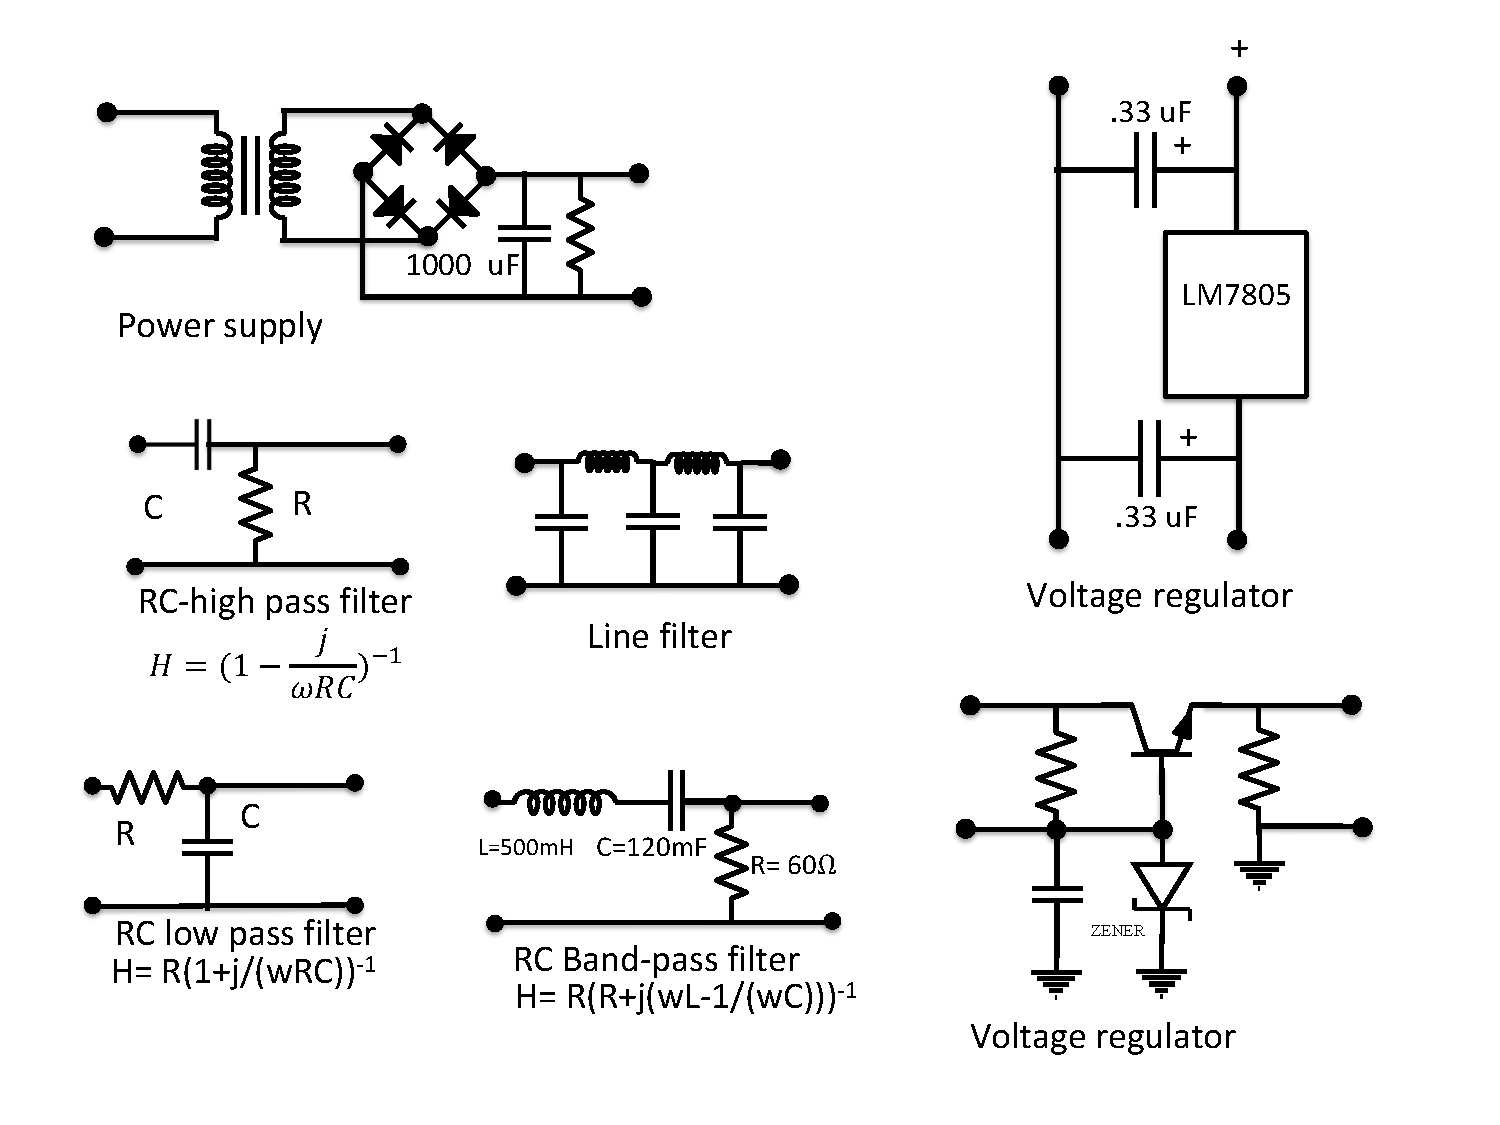
\includegraphics[width=0.8\textwidth,natwidth=642,natheight=610, height=80mm, width=88mm]{circuit1.pdf}
\end{figure}
\begin{figure} 
\center
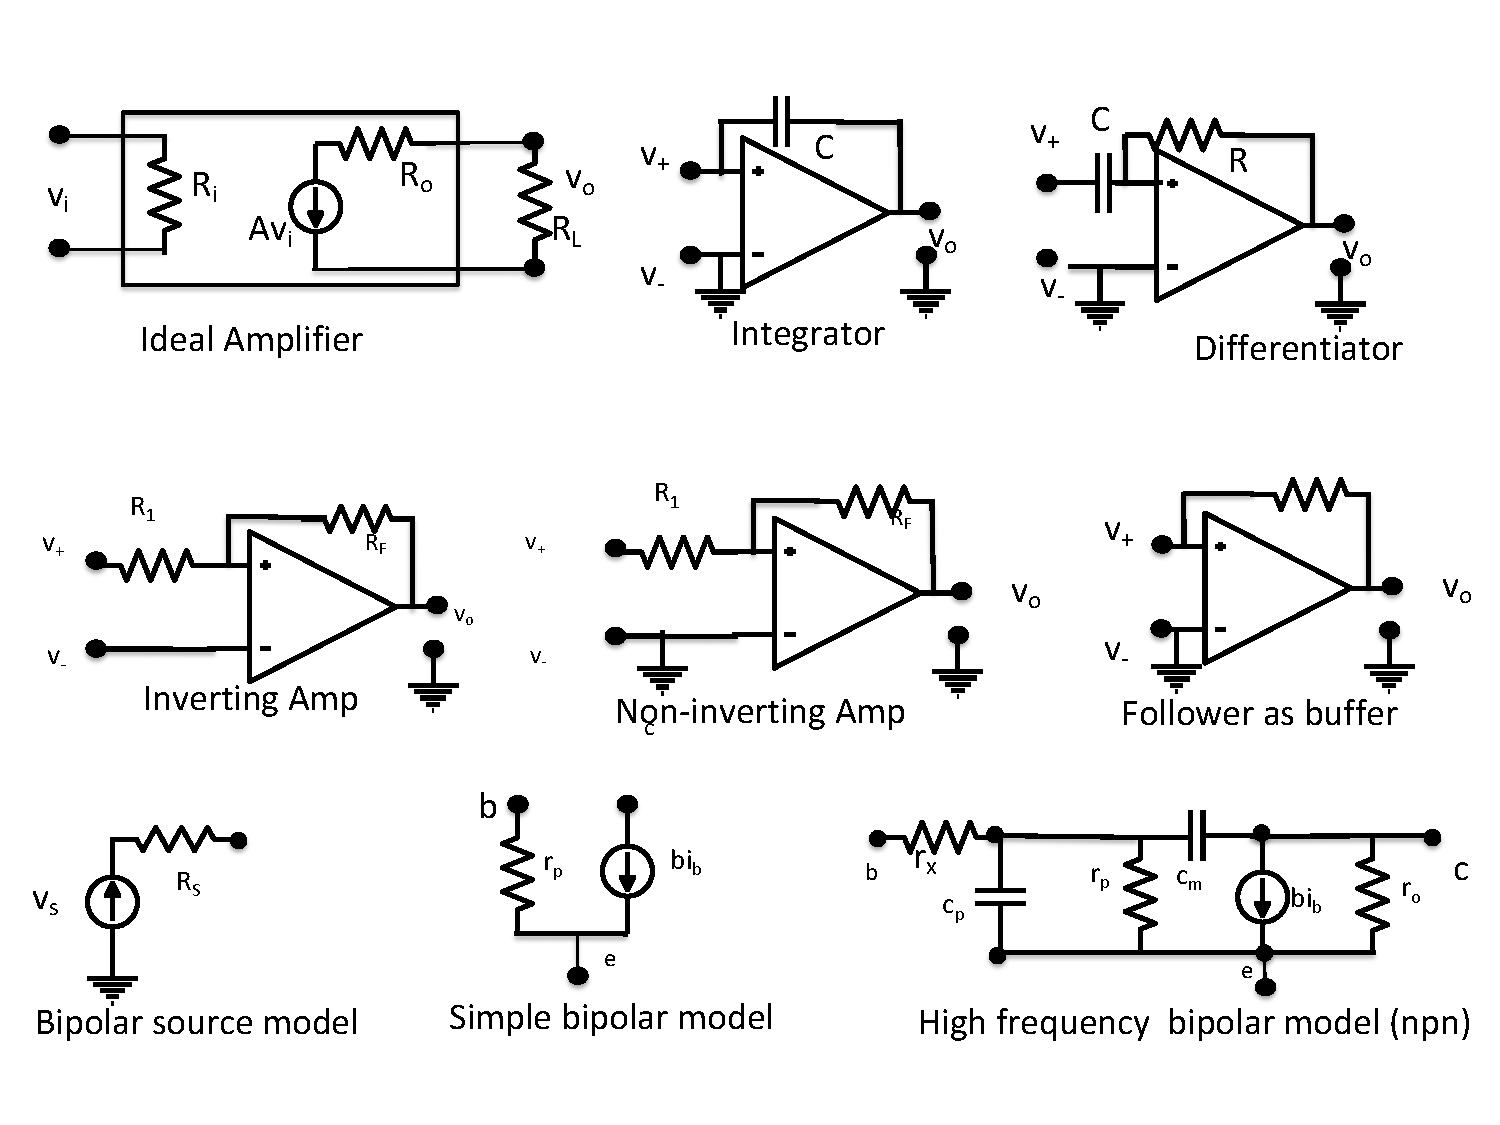
\includegraphics[width=0.8\textwidth,natwidth=642,natheight=610, height=80mm, width=88mm]{circuit2.pdf}
\end{figure}
\begin{figure} 
\center
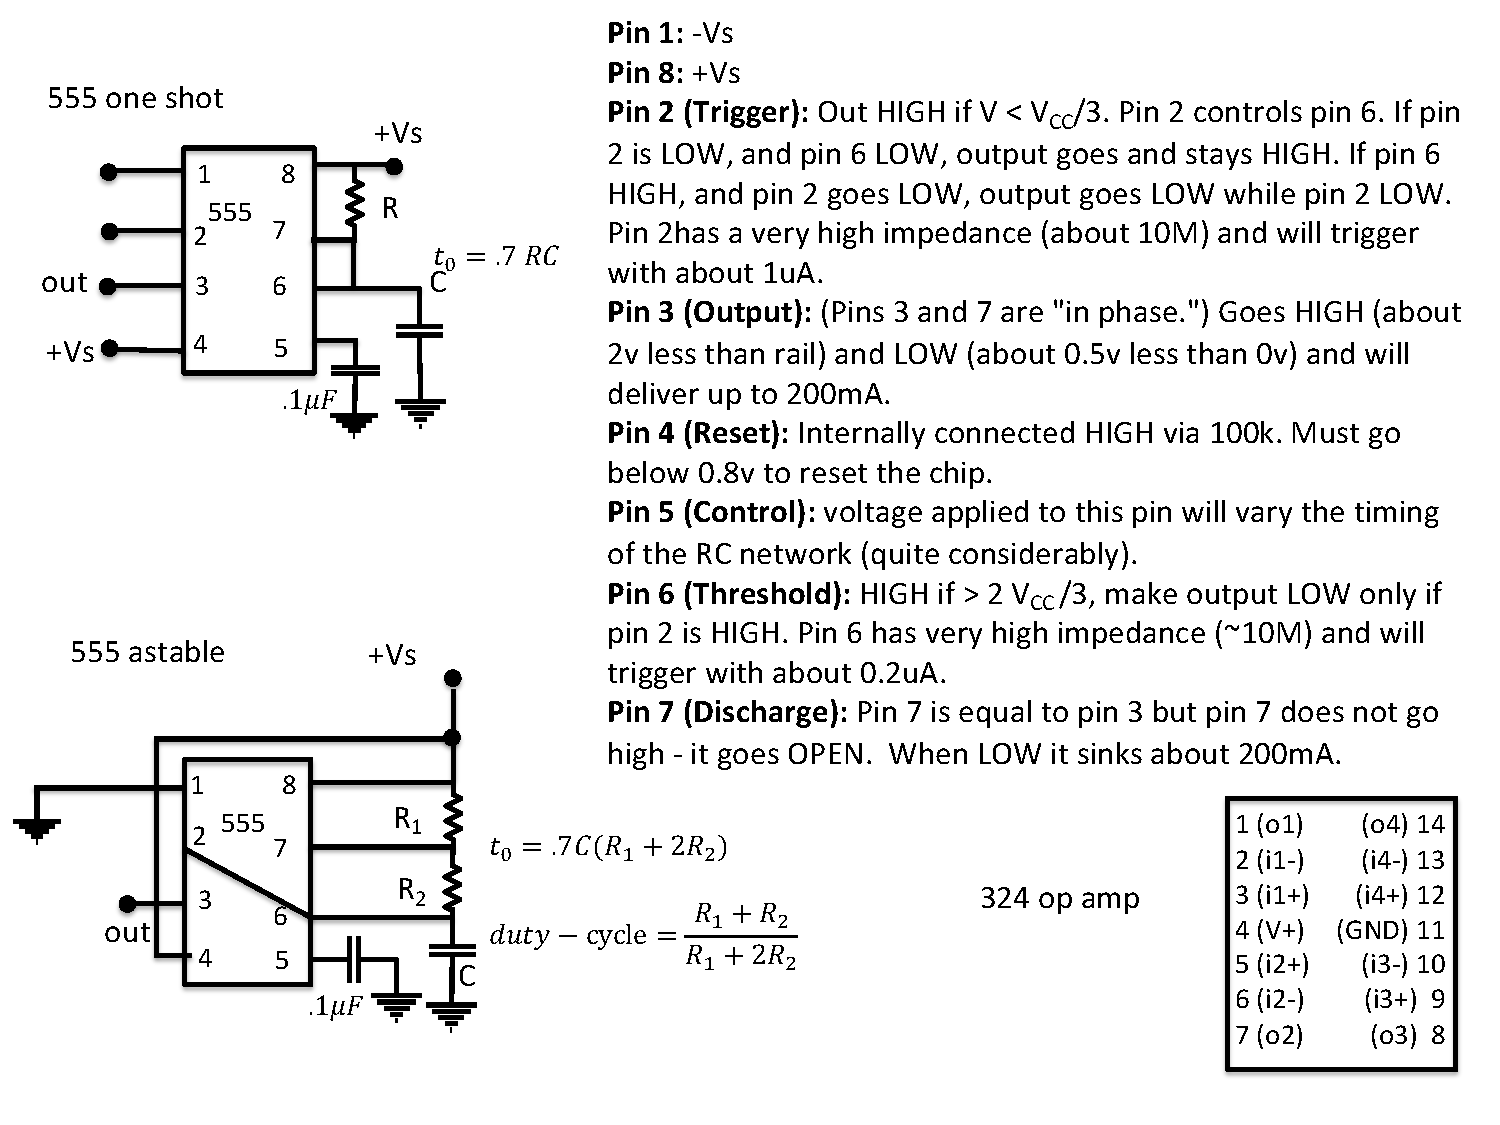
\includegraphics[width=0.8\textwidth,natwidth=642,natheight=610, height=80mm, width=88mm]{circuit3.pdf}
\end{figure}
\begin{figure} 
\center
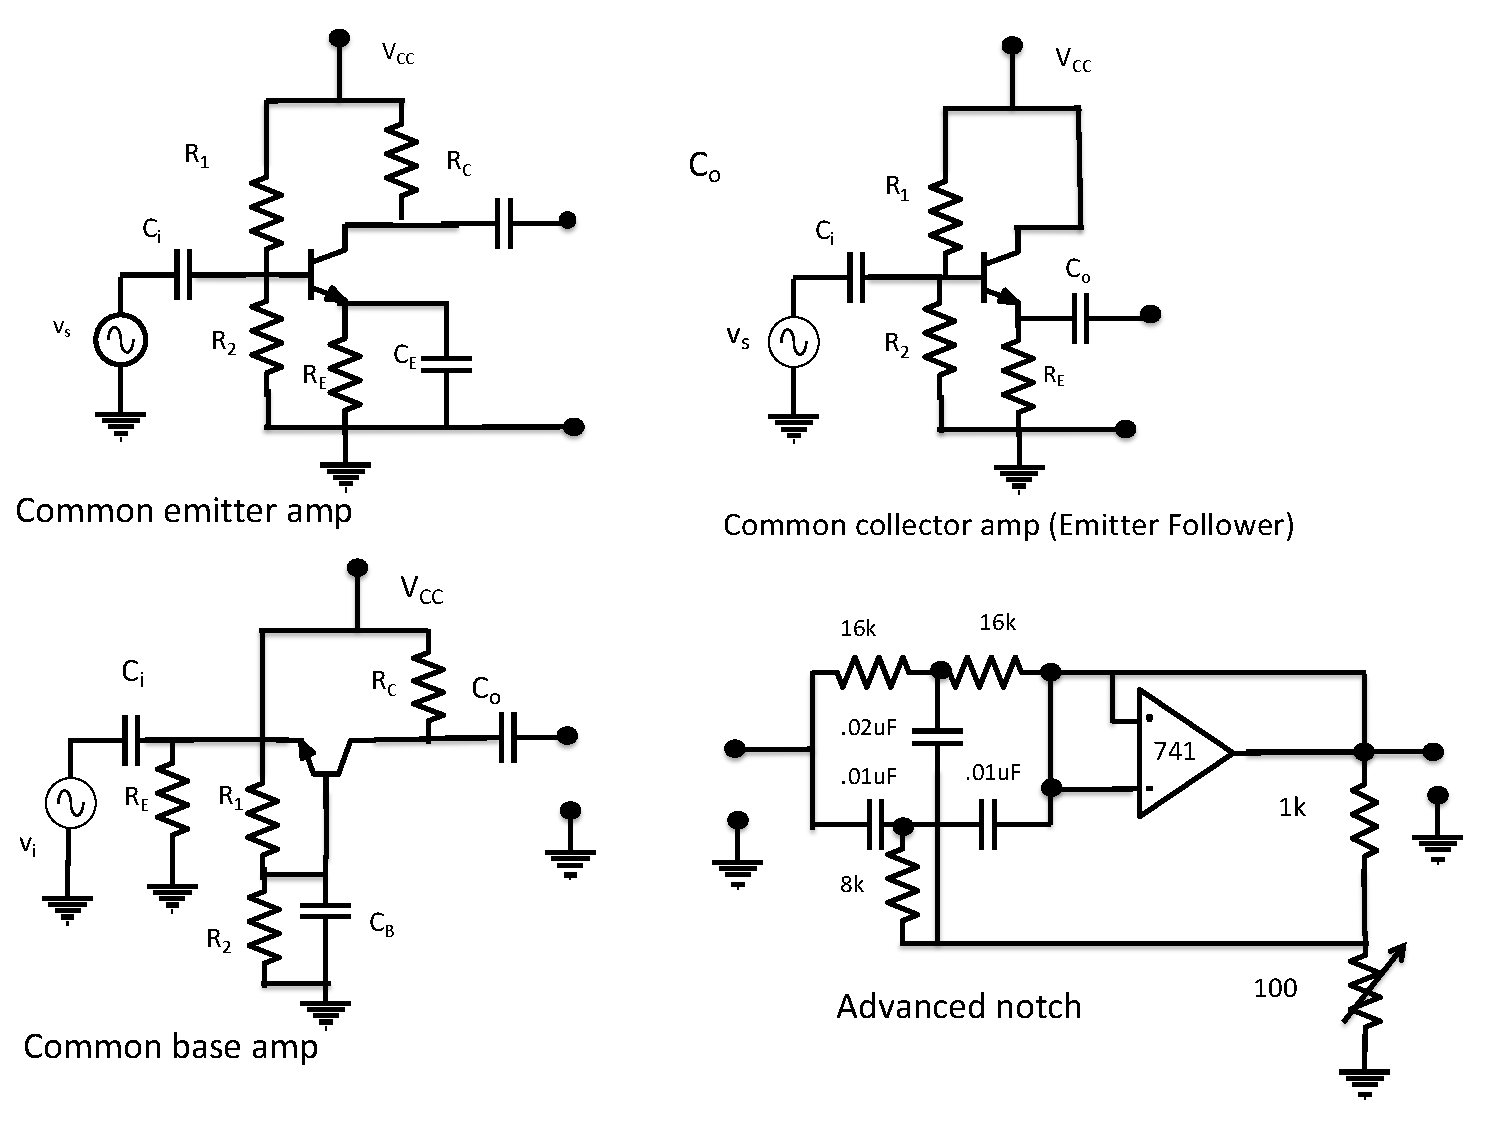
\includegraphics[width=0.8\textwidth,natwidth=642,natheight=610, height=80mm, width=88mm]{circuit4.pdf}
\end{figure}
\begin{figure} 
\center
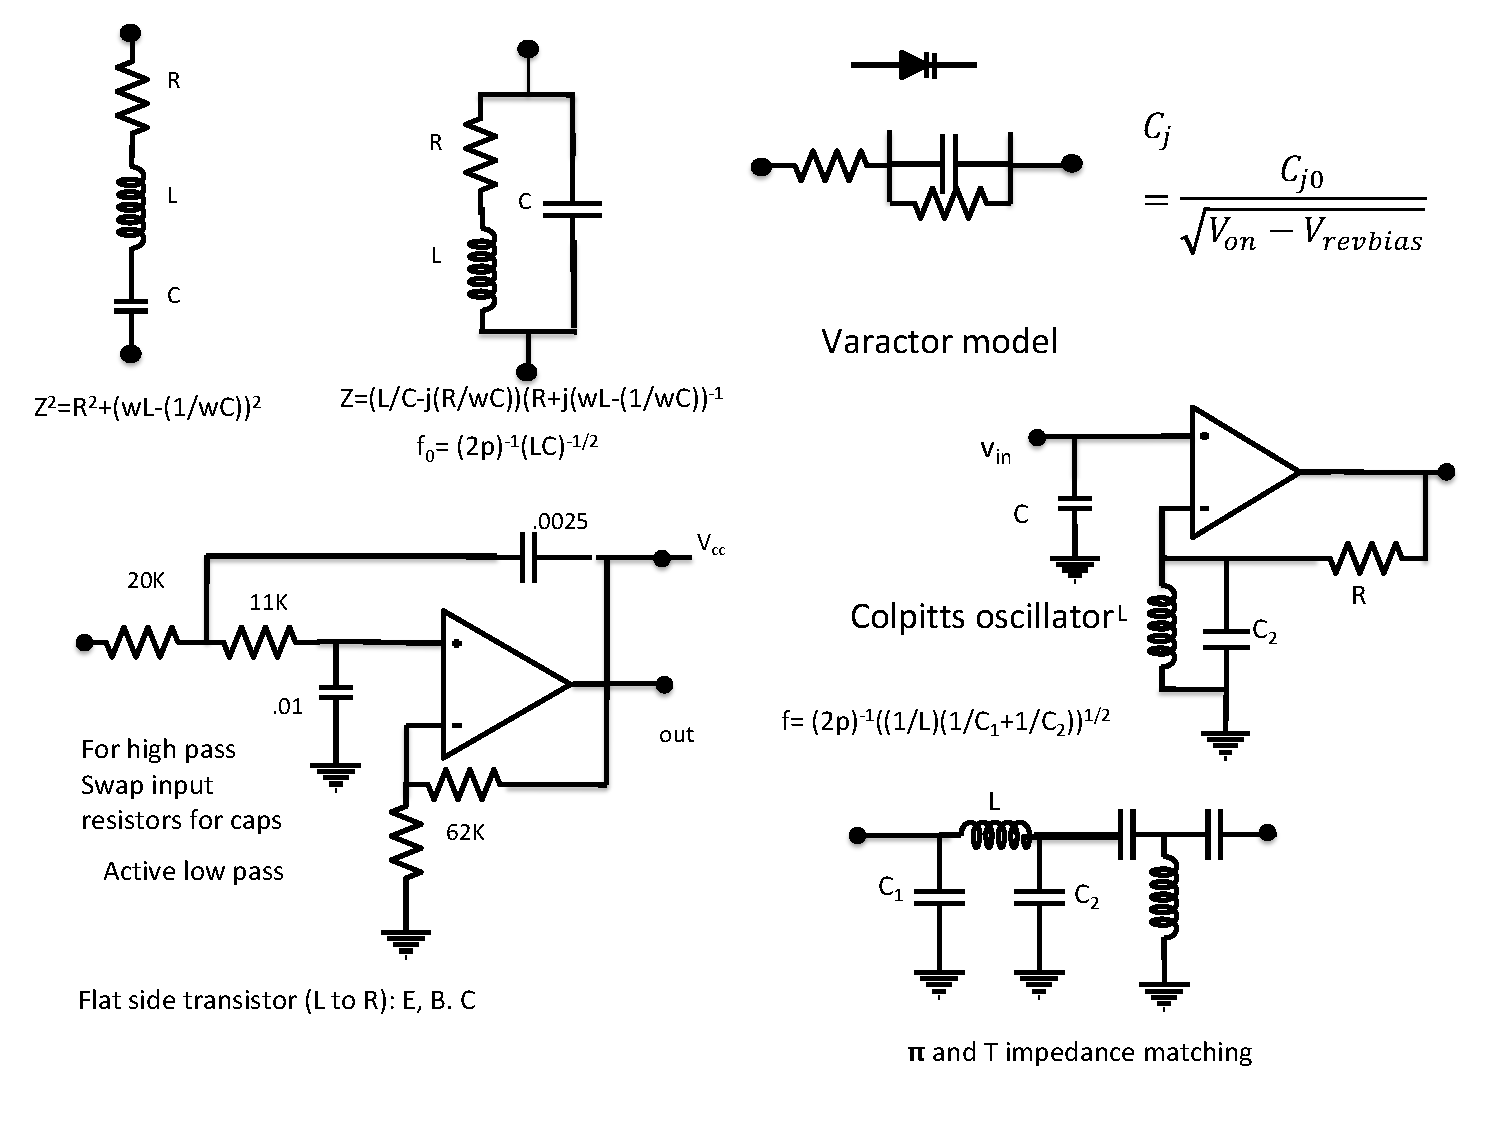
\includegraphics[width=0.8\textwidth,natwidth=642,natheight=610, height=80mm, width=88mm]{circuit5.pdf}
\end{figure}
\begin{figure} 
\center
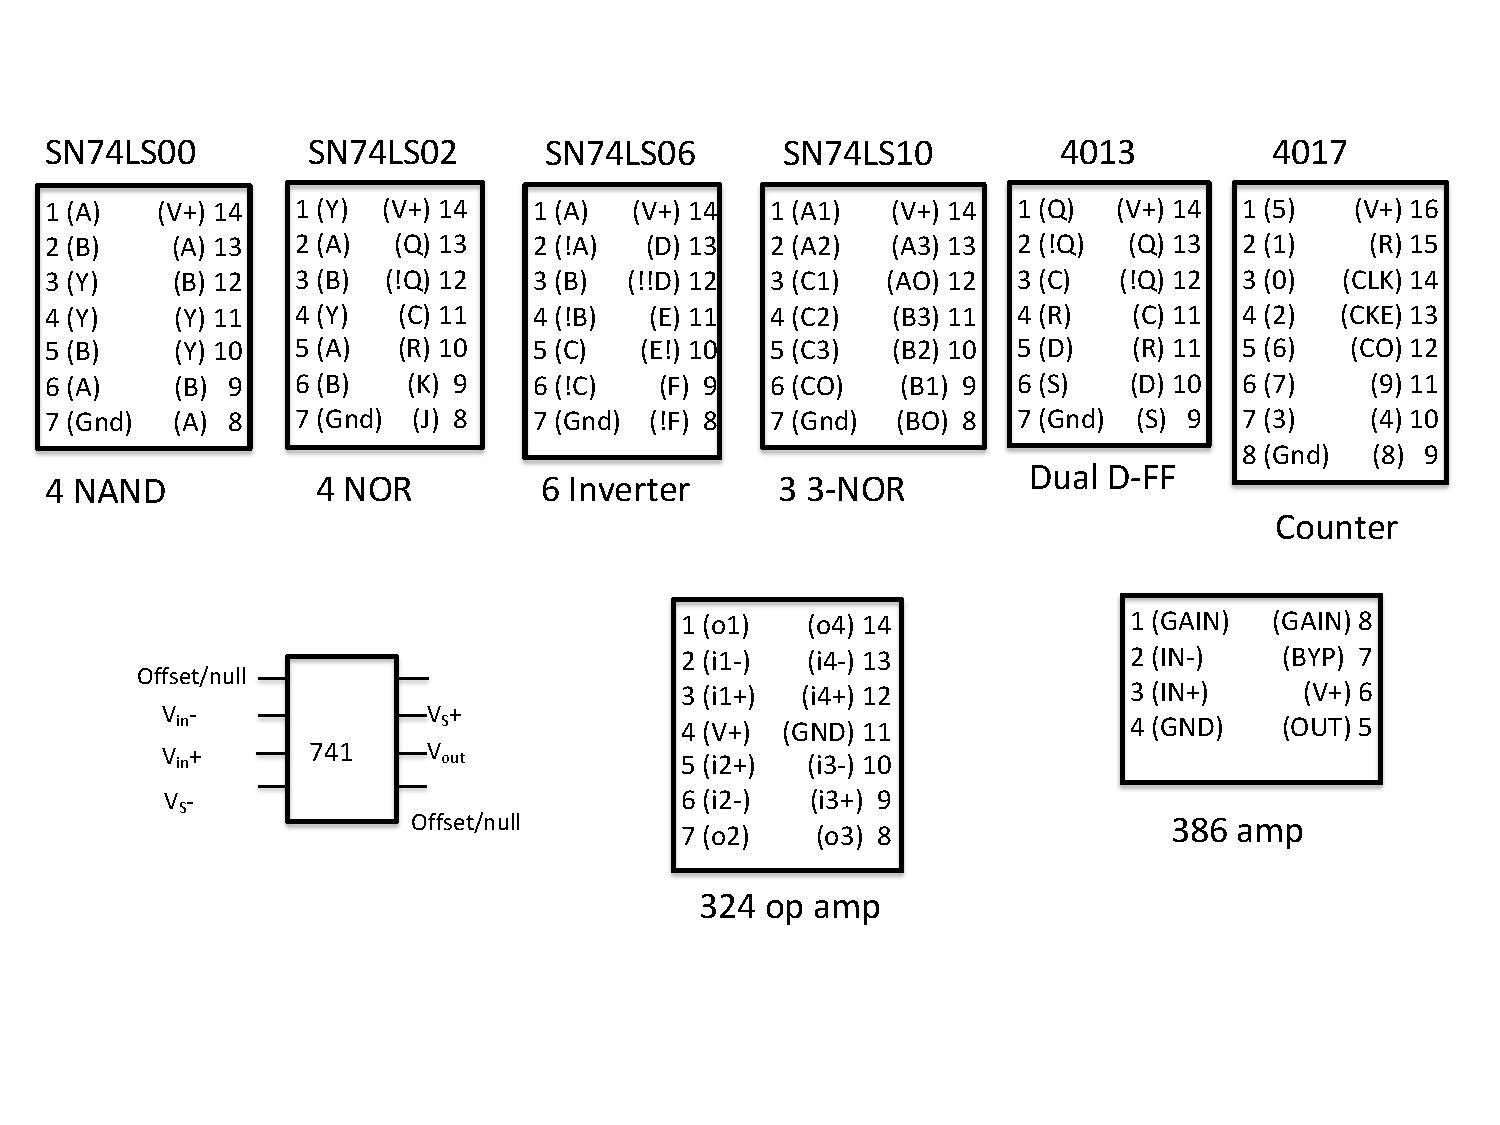
\includegraphics[width=0.8\textwidth,natwidth=642,natheight=610, height=80mm, width=88mm]{circuit6.pdf}
\end{figure}
\begin{figure} 
\center
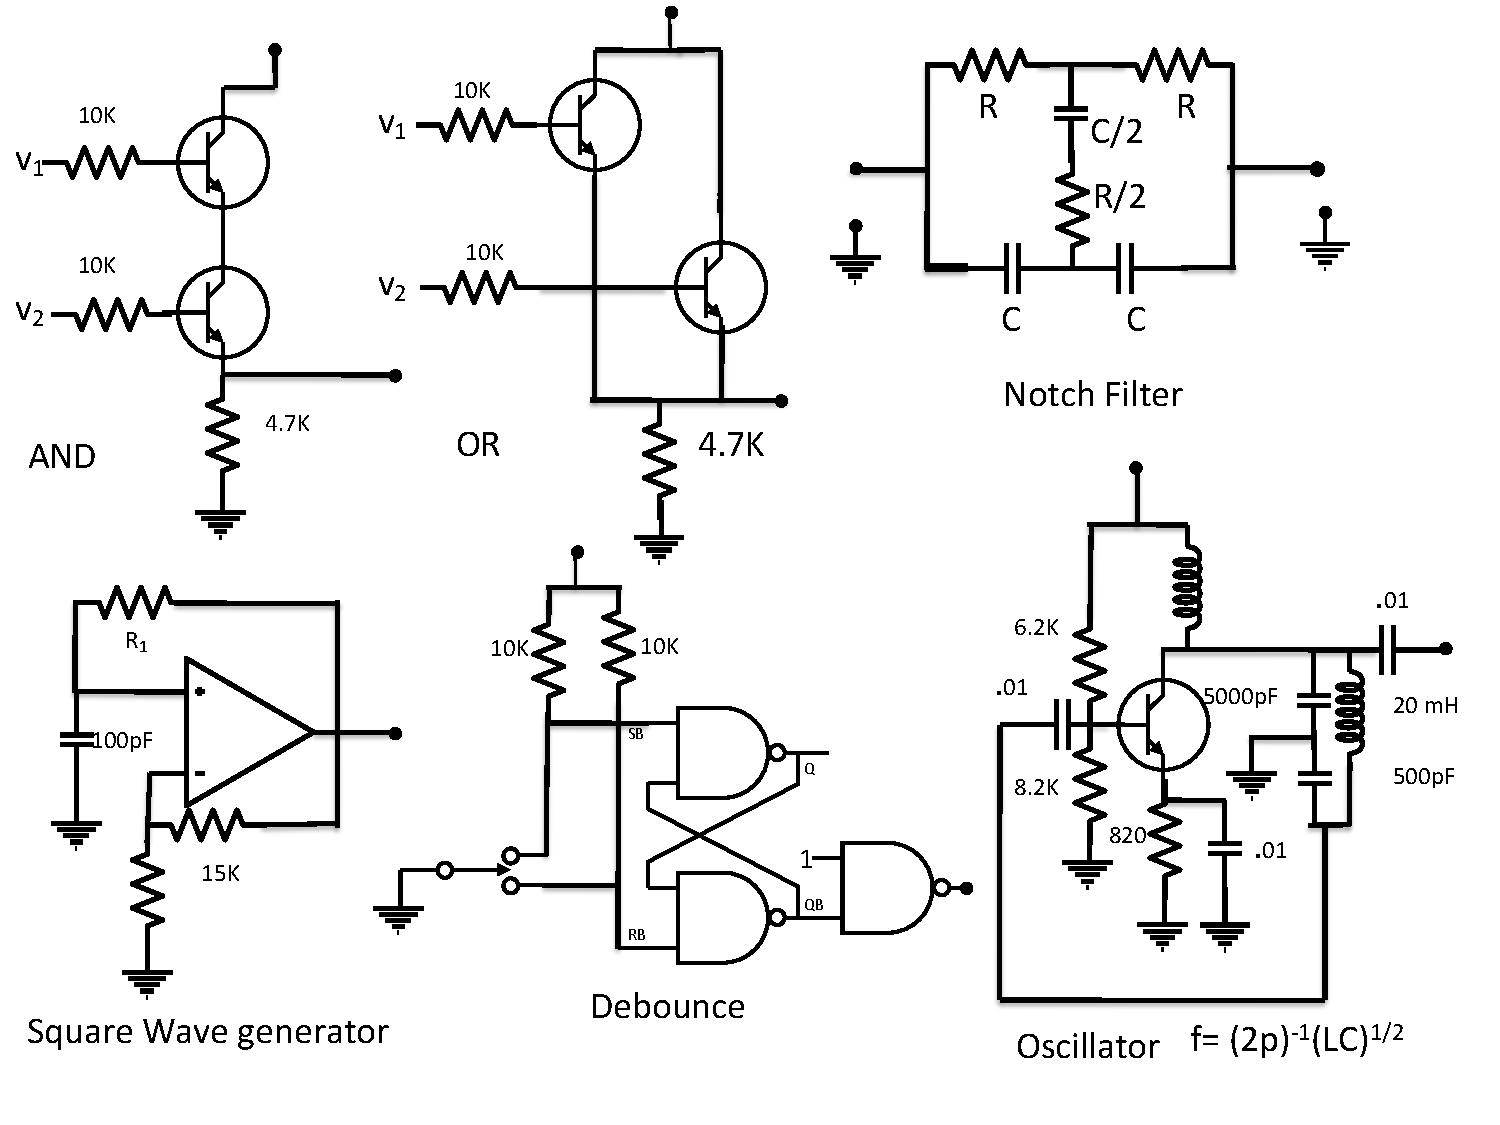
\includegraphics[width=0.8\textwidth,natwidth=642,natheight=610, height=80mm, width=88mm]{circuit7.pdf}
\end{figure}
\begin{figure} 
\center
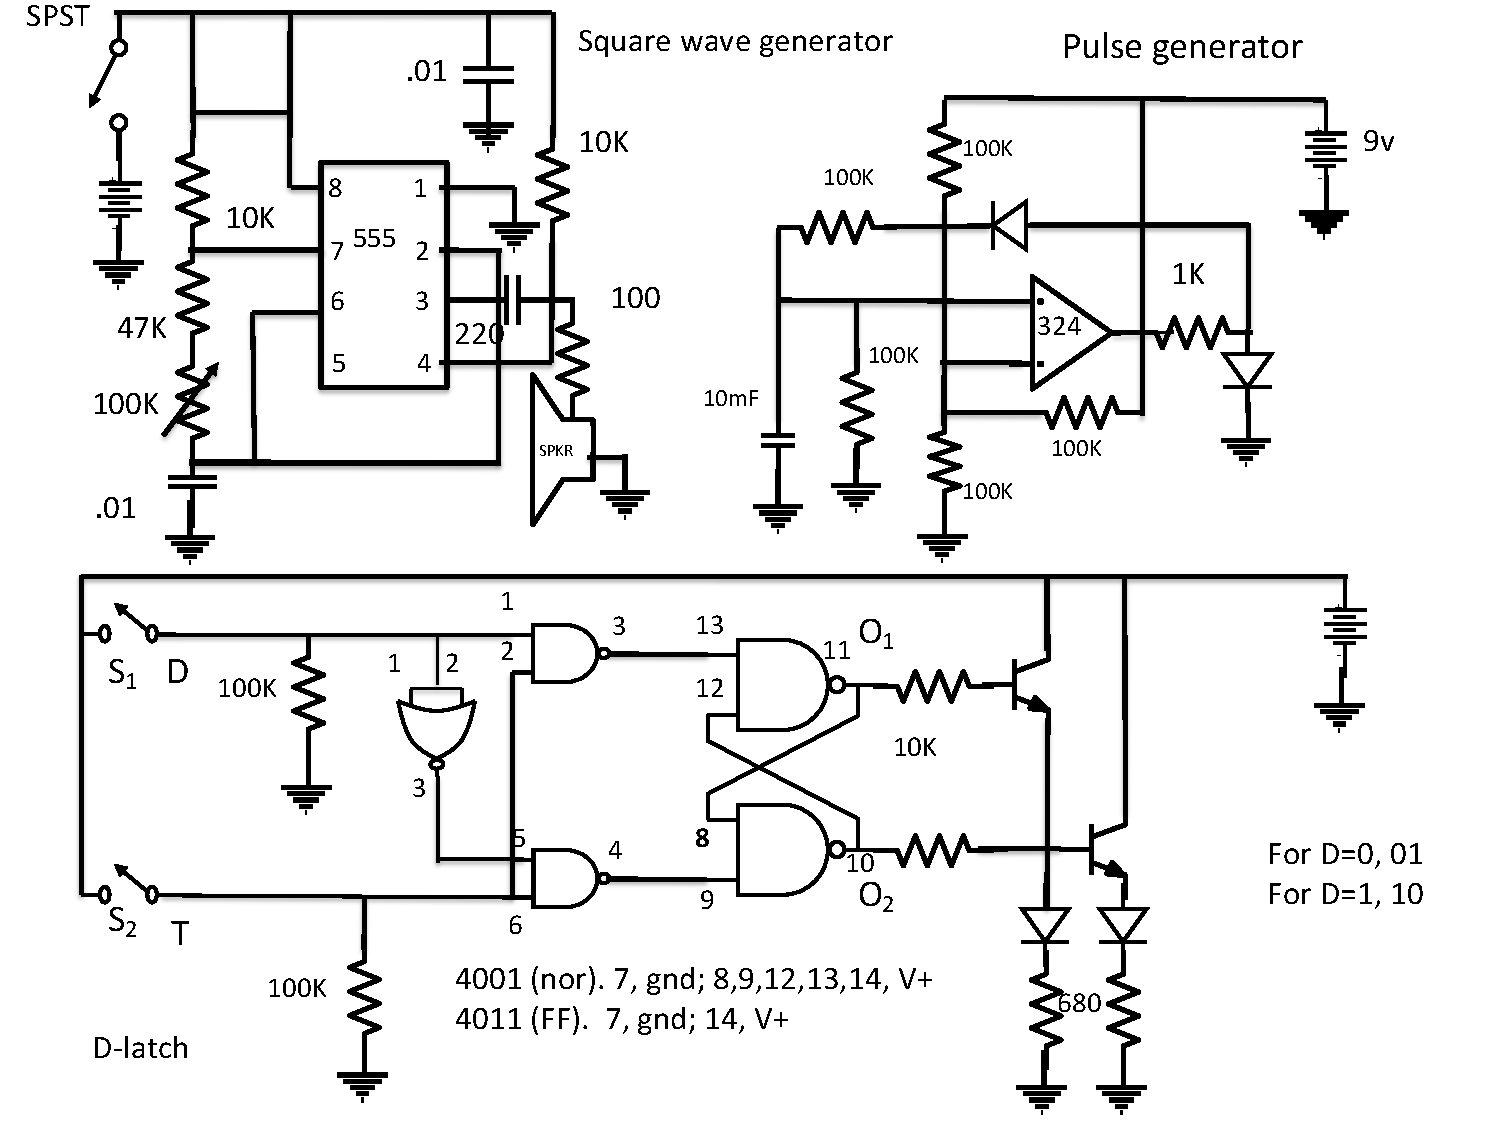
\includegraphics[width=0.8\textwidth,natwidth=642,natheight=610, height=80mm, width=88mm]{circuit8.pdf}
\end{figure}
\begin{figure} 
\center
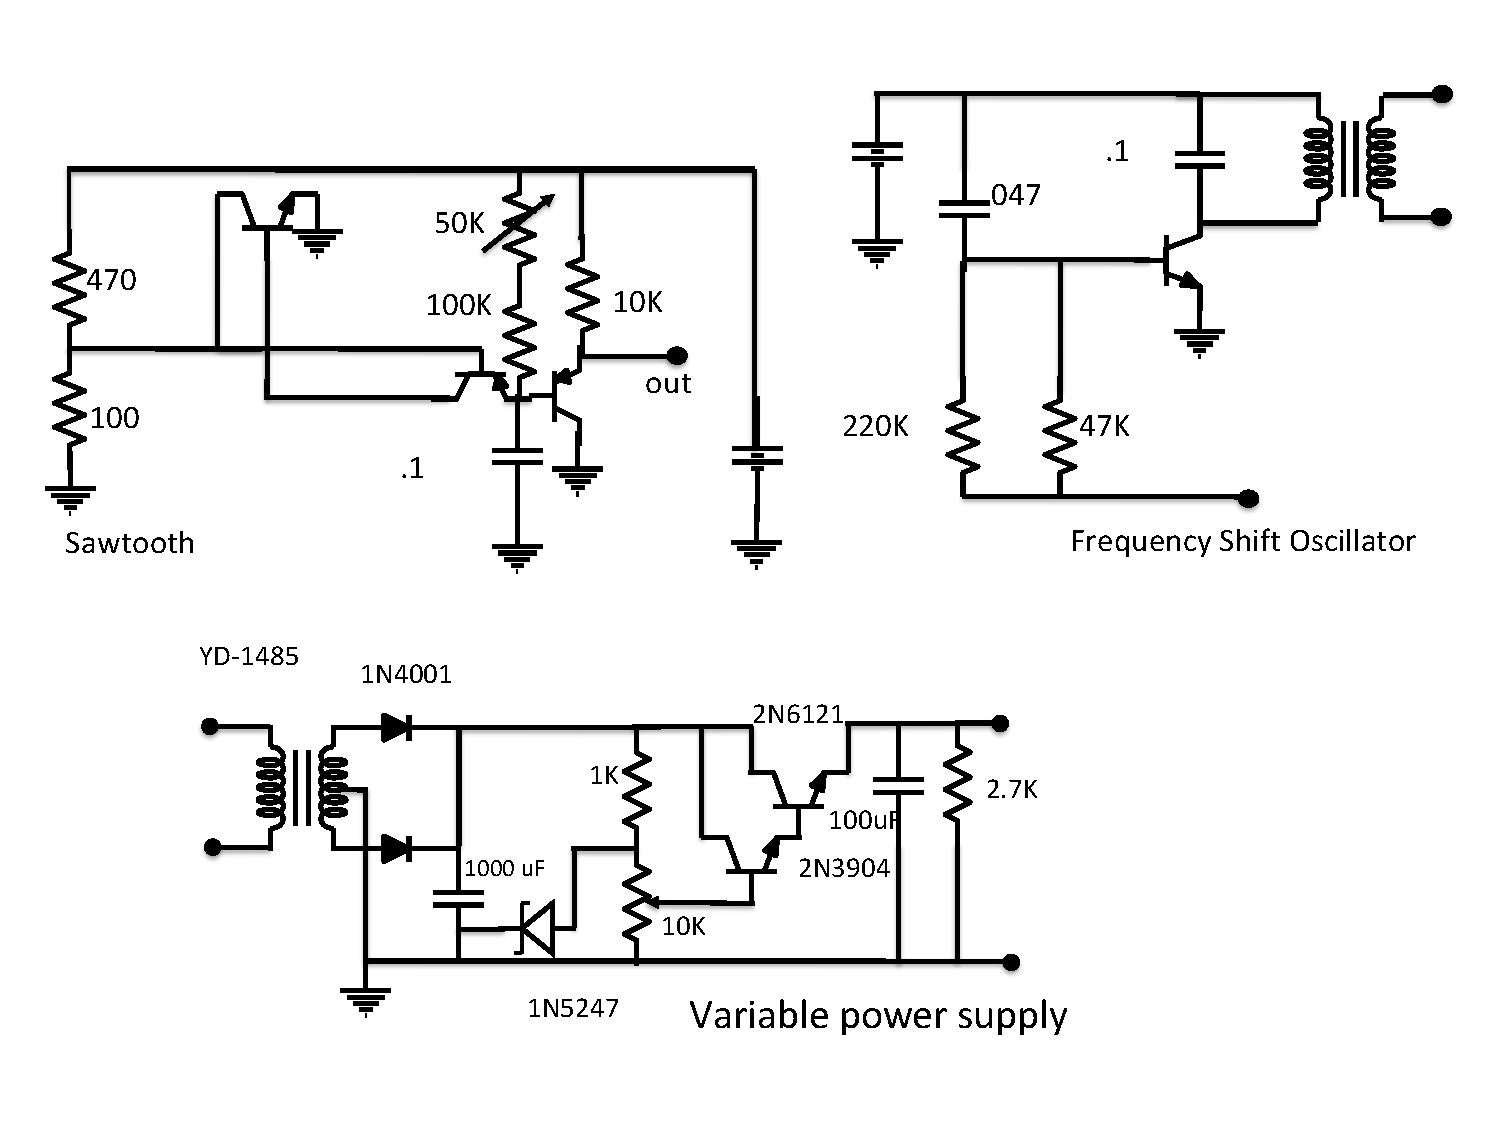
\includegraphics[width=0.8\textwidth,natwidth=642,natheight=610, height=80mm, width=88mm]{circuit9.pdf}
\end{figure}
\begin{figure} 
\center
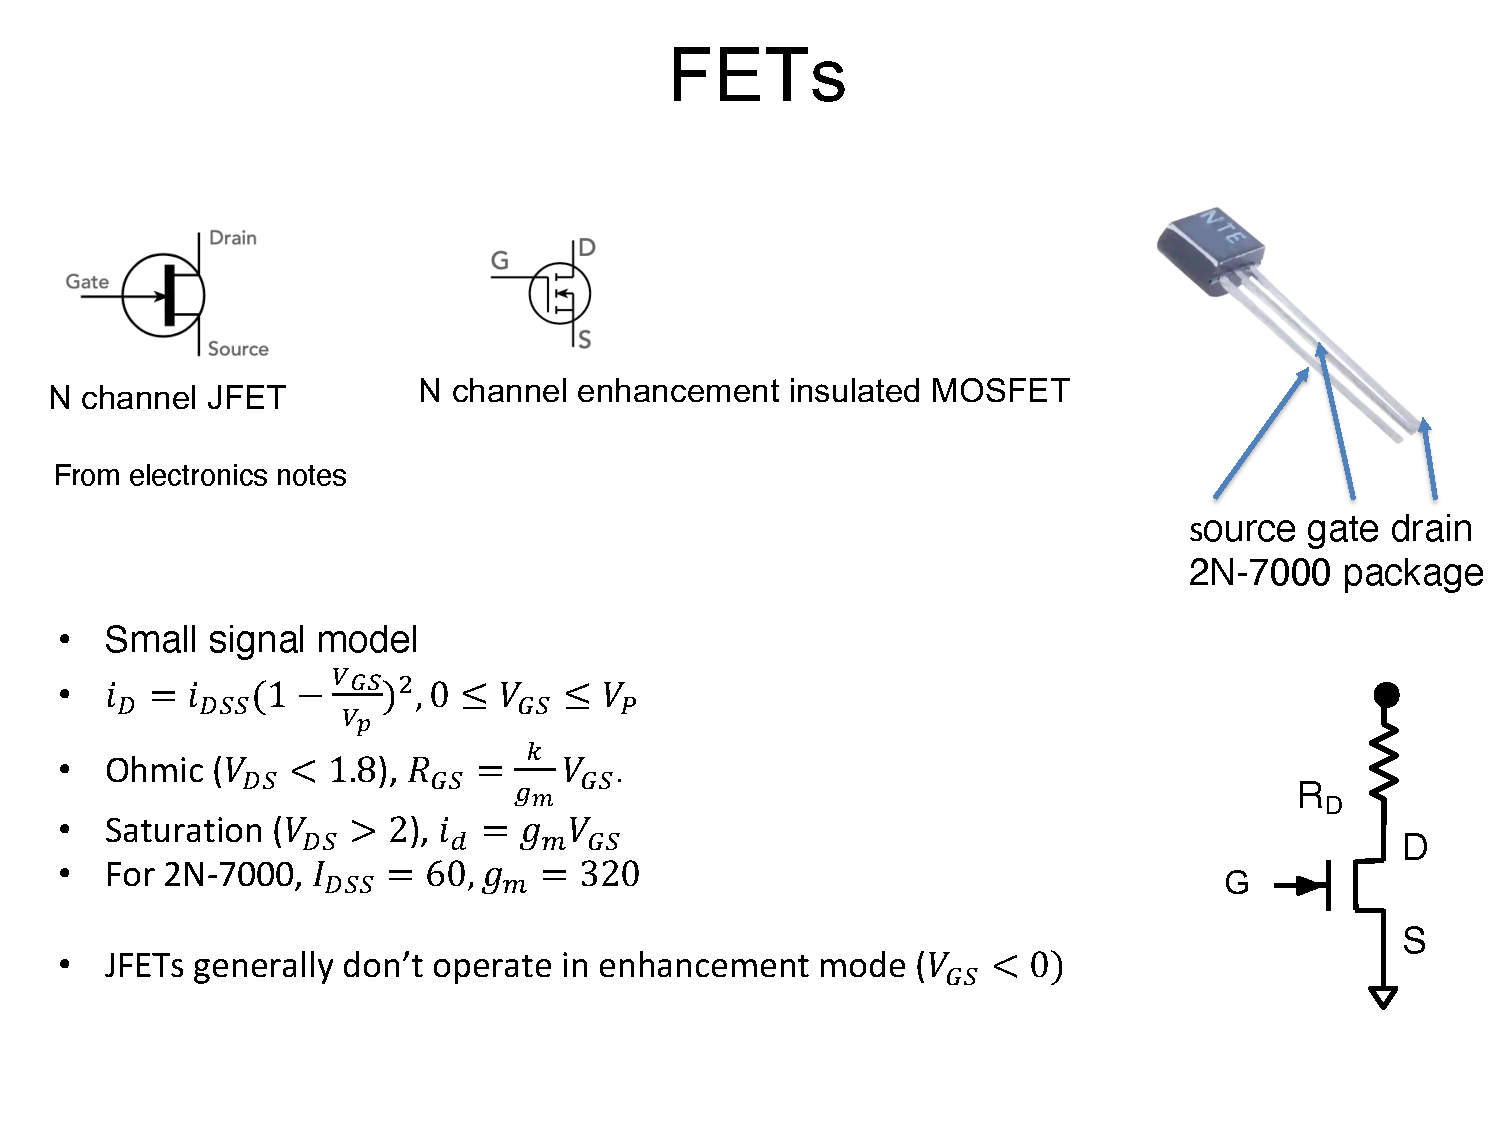
\includegraphics[width=0.8\textwidth,natwidth=642,natheight=610, height=80mm, width=88mm]{circuit10.pdf}
\end{figure}
\begin{figure} 
\center
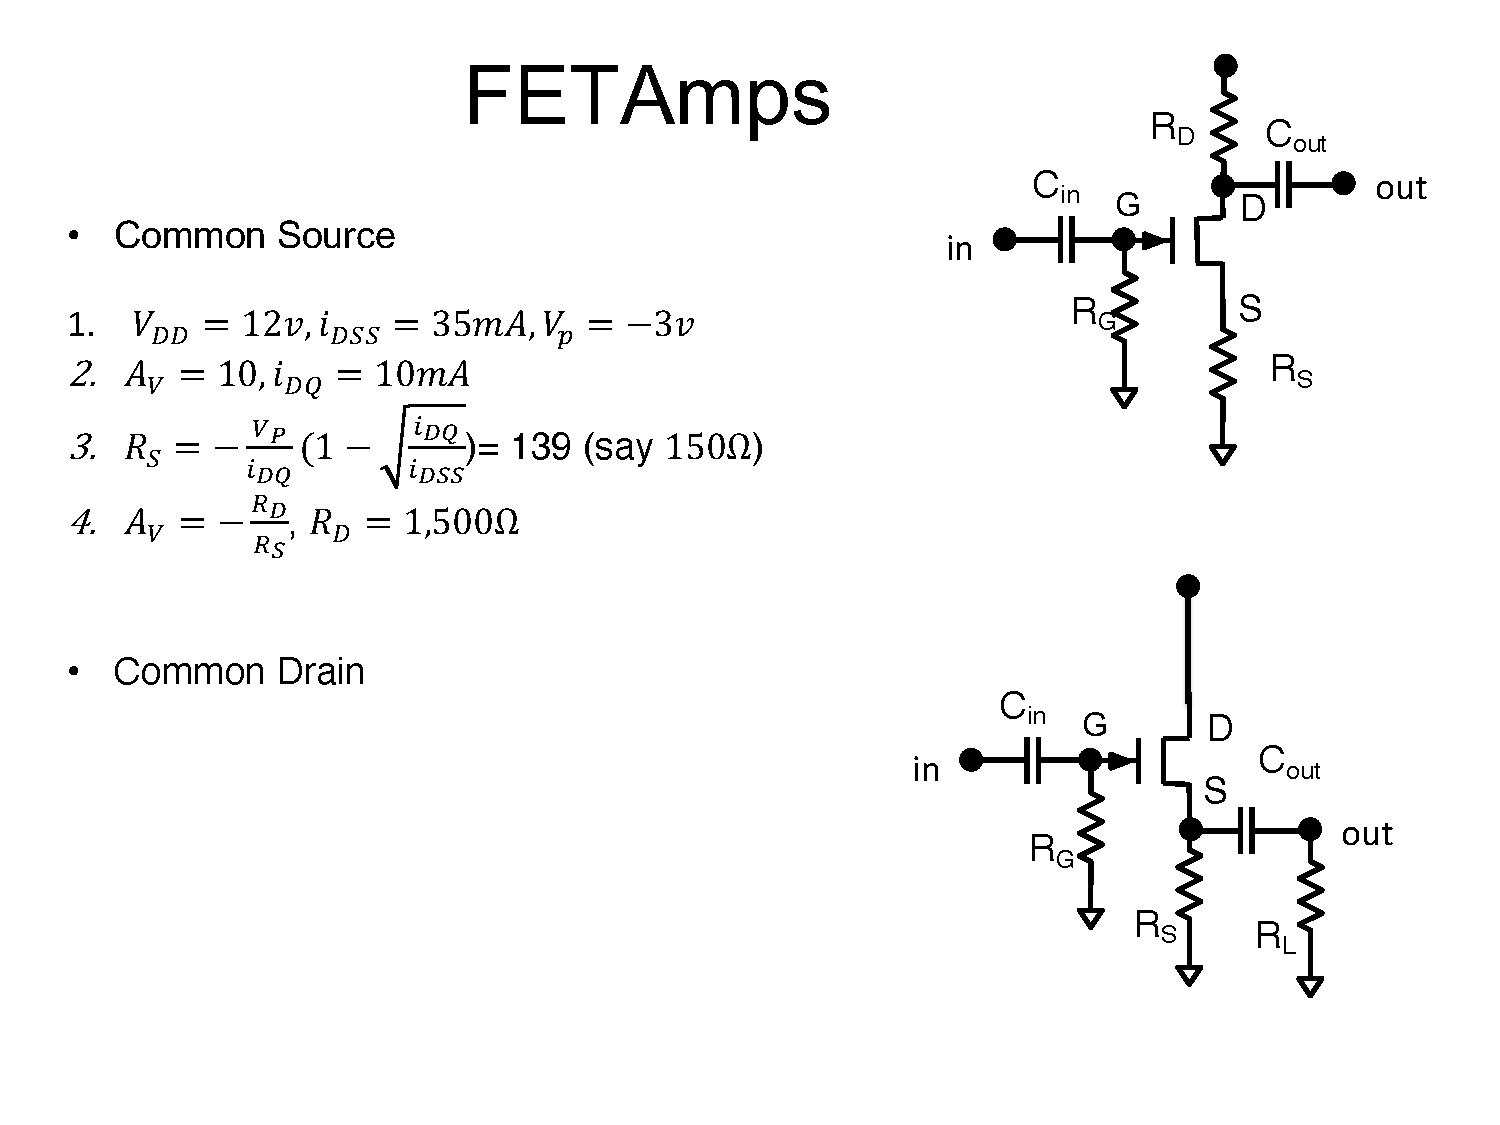
\includegraphics[width=0.8\textwidth,natwidth=642,natheight=610, height=80mm, width=88mm]{circuit11.pdf}
\end{figure}
\begin{figure} 
\center
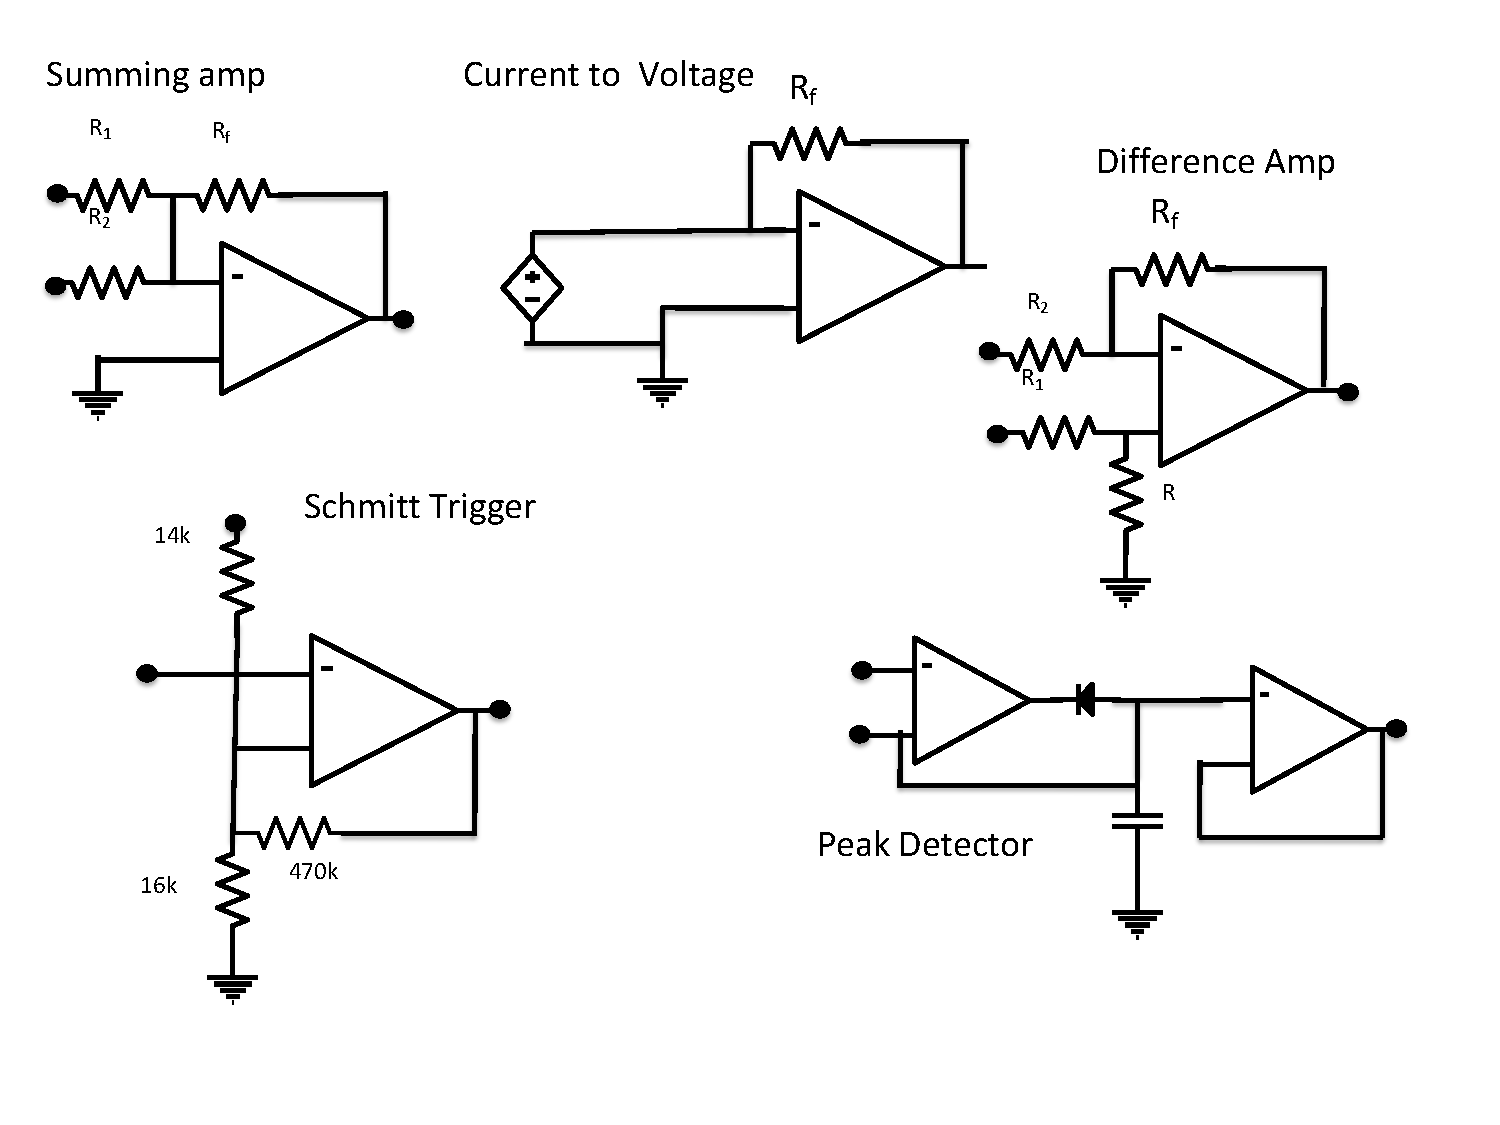
\includegraphics[width=0.8\textwidth,natwidth=642,natheight=610, height=80mm, width=88mm]{circuit12.pdf}
\end{figure}
\begin{figure} 
\center
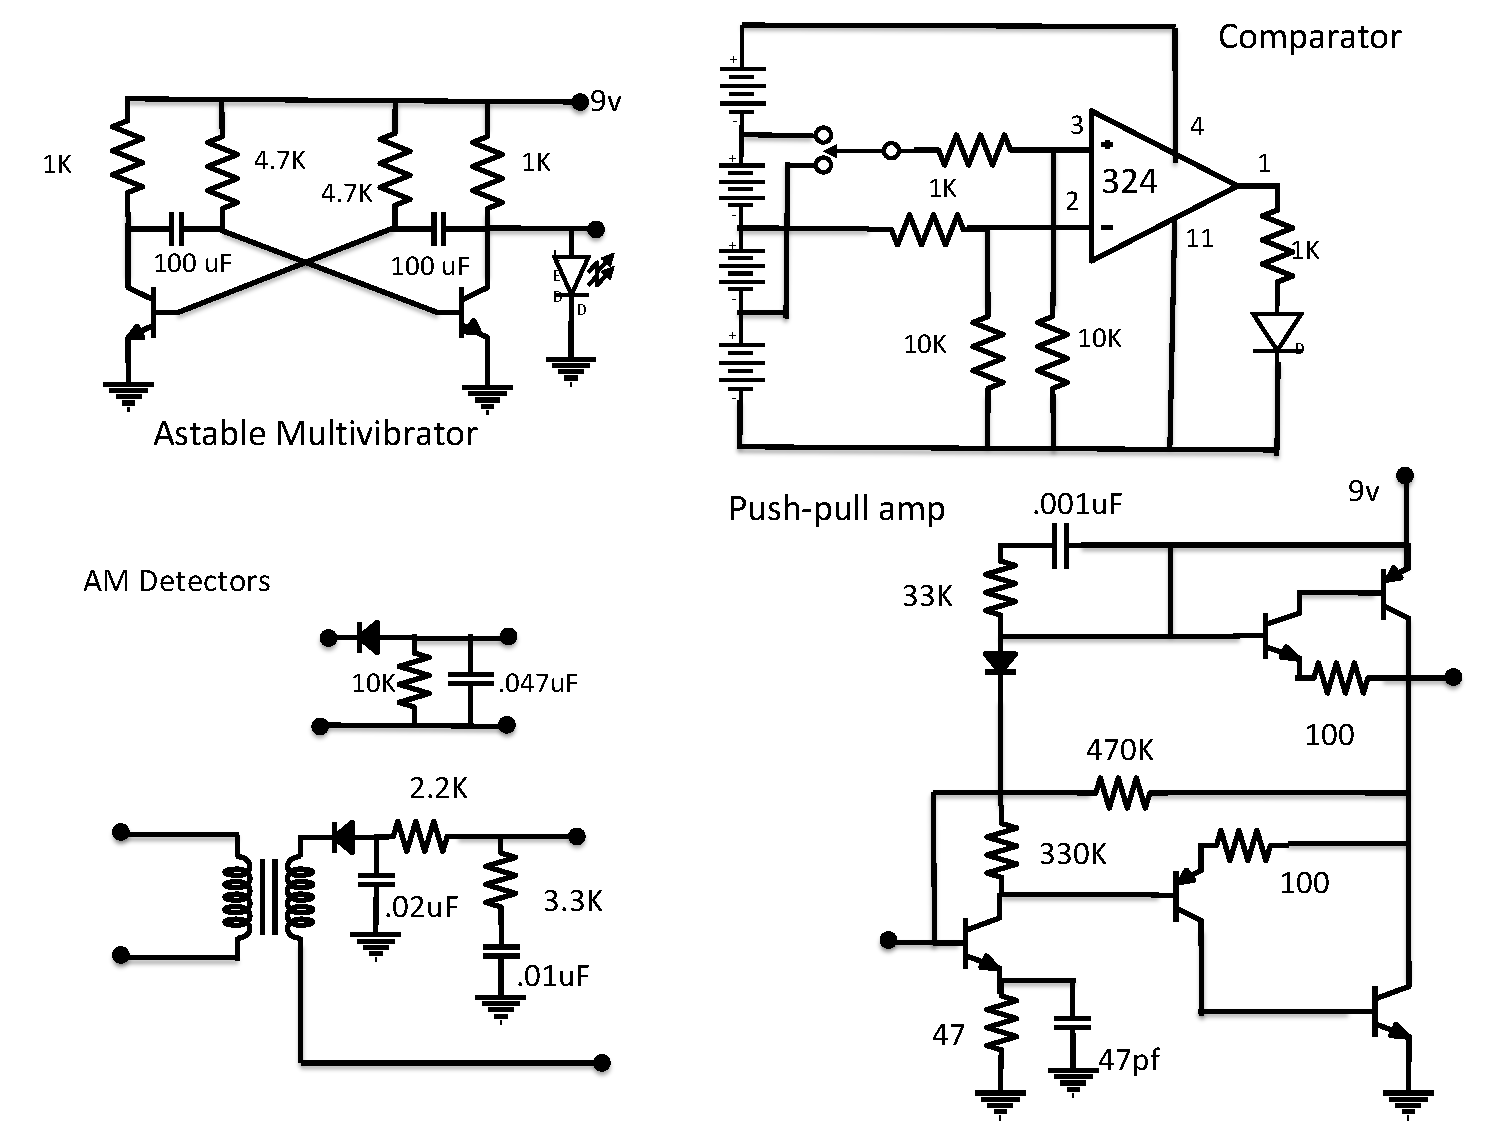
\includegraphics[width=0.8\textwidth,natwidth=642,natheight=610, height=80mm, width=88mm]{circuit13.pdf}
\end{figure}
\begin{figure} 
\center
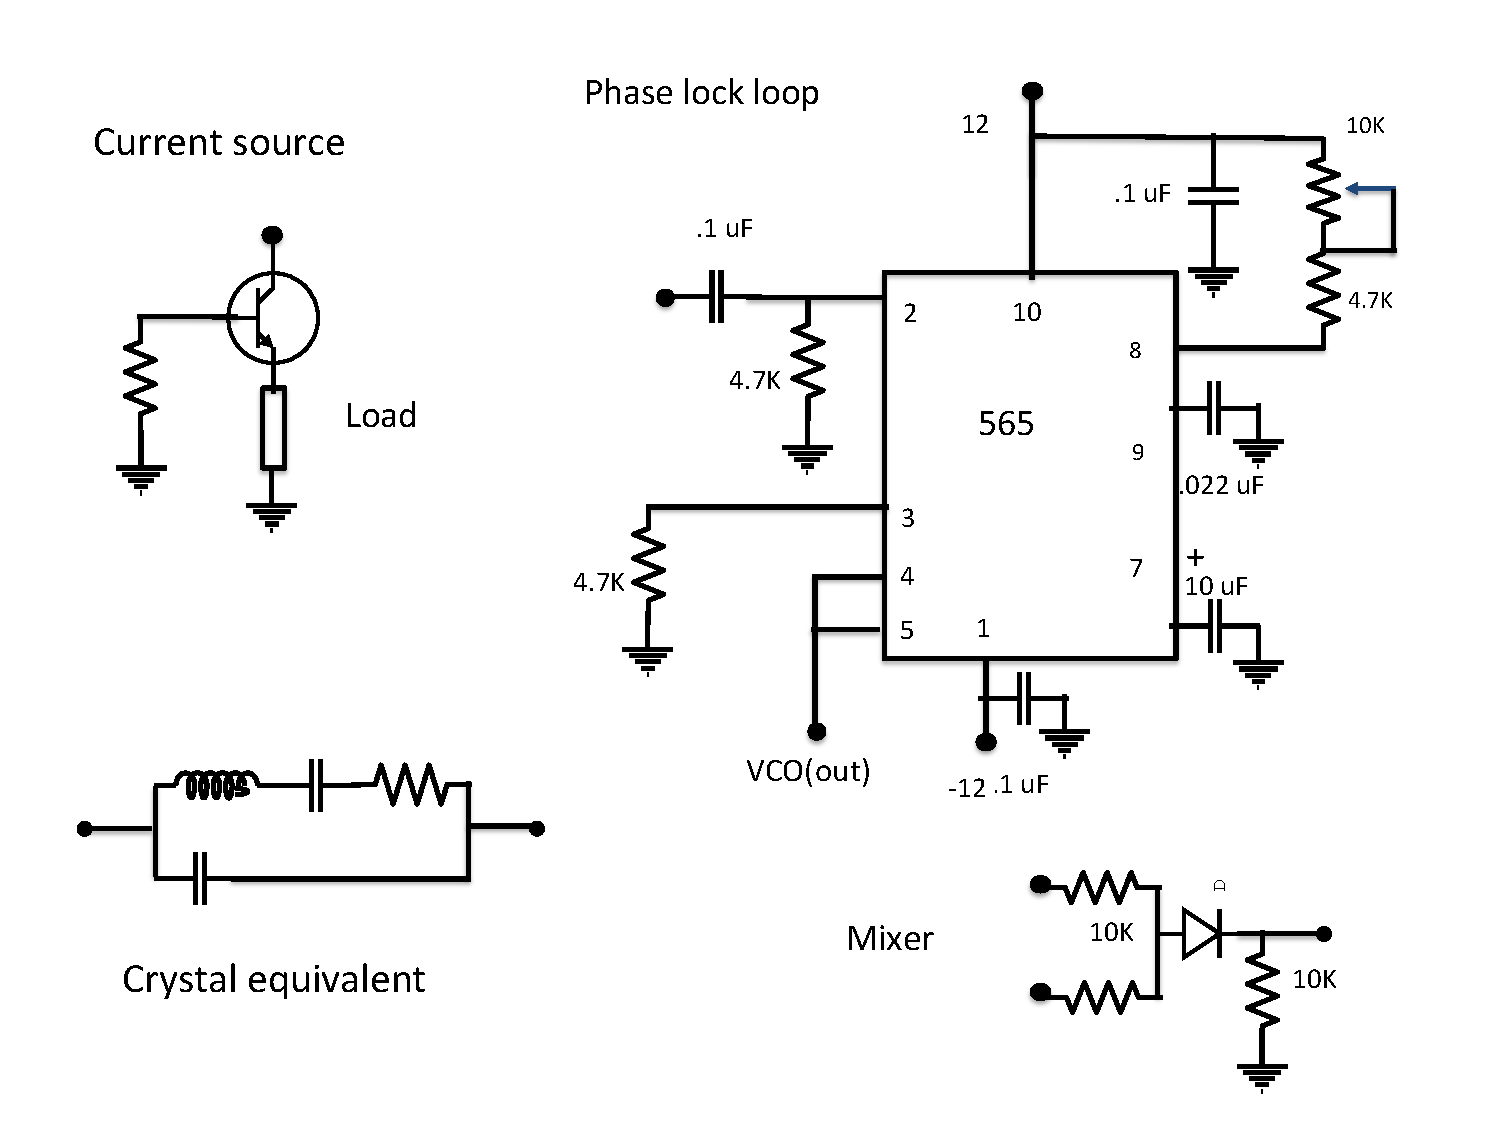
\includegraphics[width=0.8\textwidth,natwidth=642,natheight=610, height=80mm, width=88mm]{circuit14.pdf}
\end{figure}
\begin{figure} 
\center
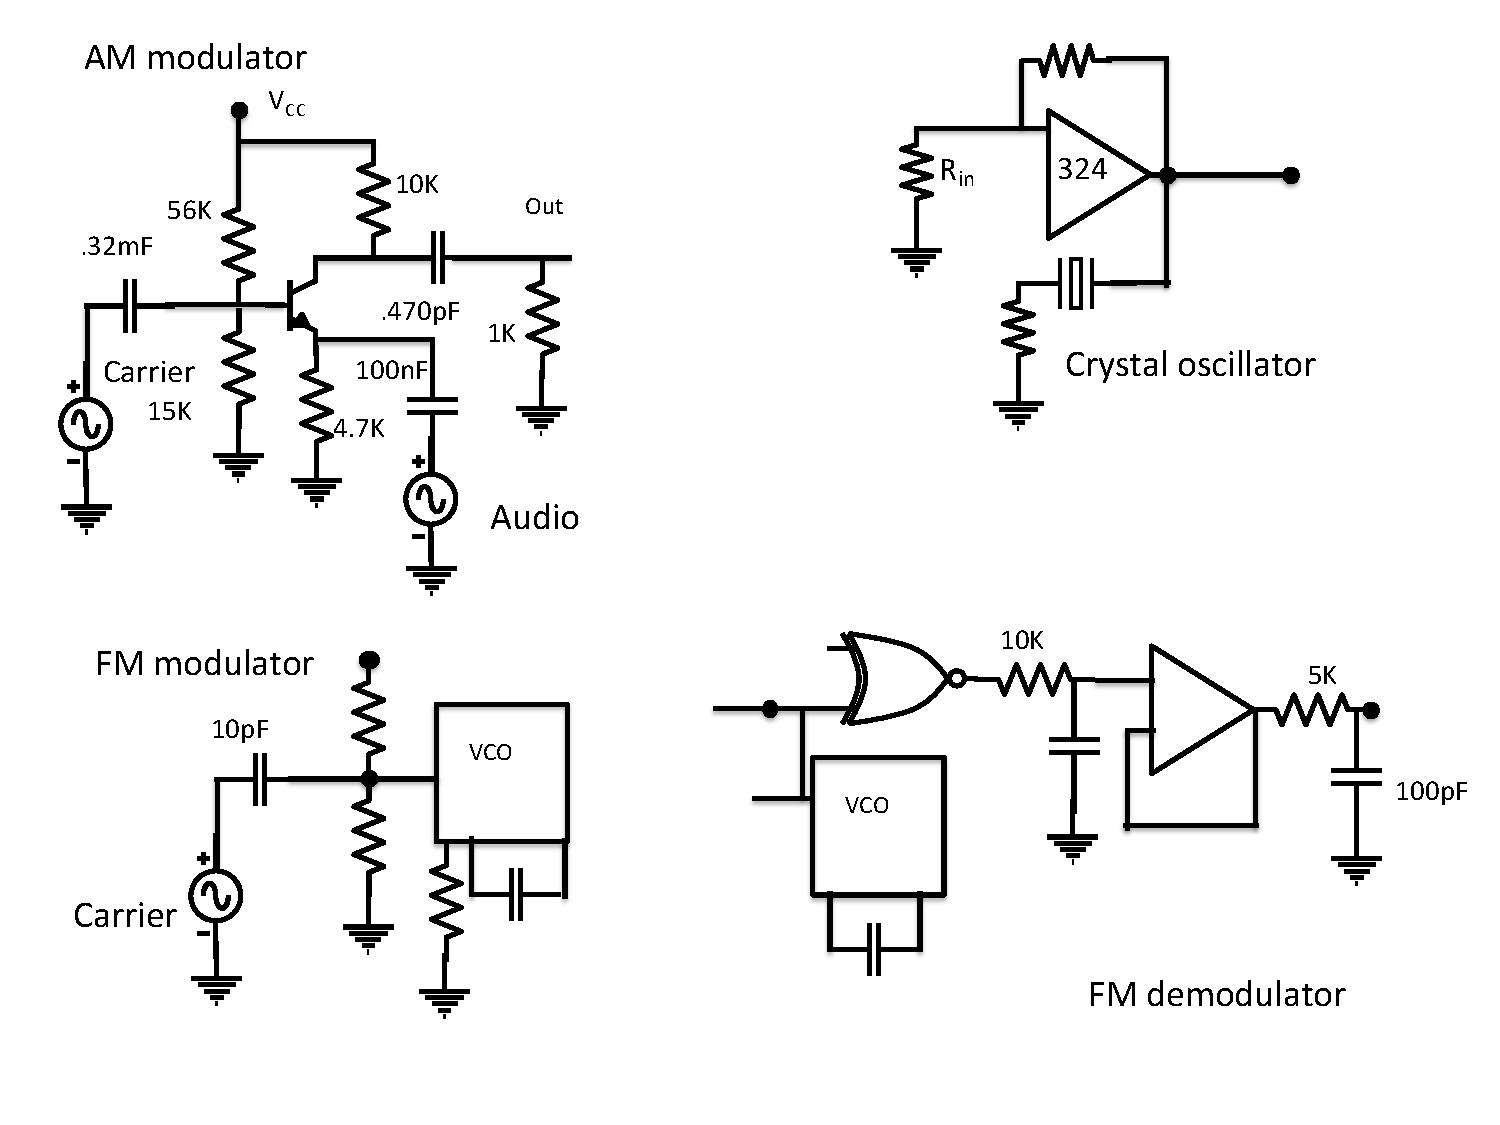
\includegraphics[width=0.8\textwidth,natwidth=642,natheight=610, height=80mm, width=88mm]{circuit15.pdf}
\end{figure}
\begin{figure} 
\center
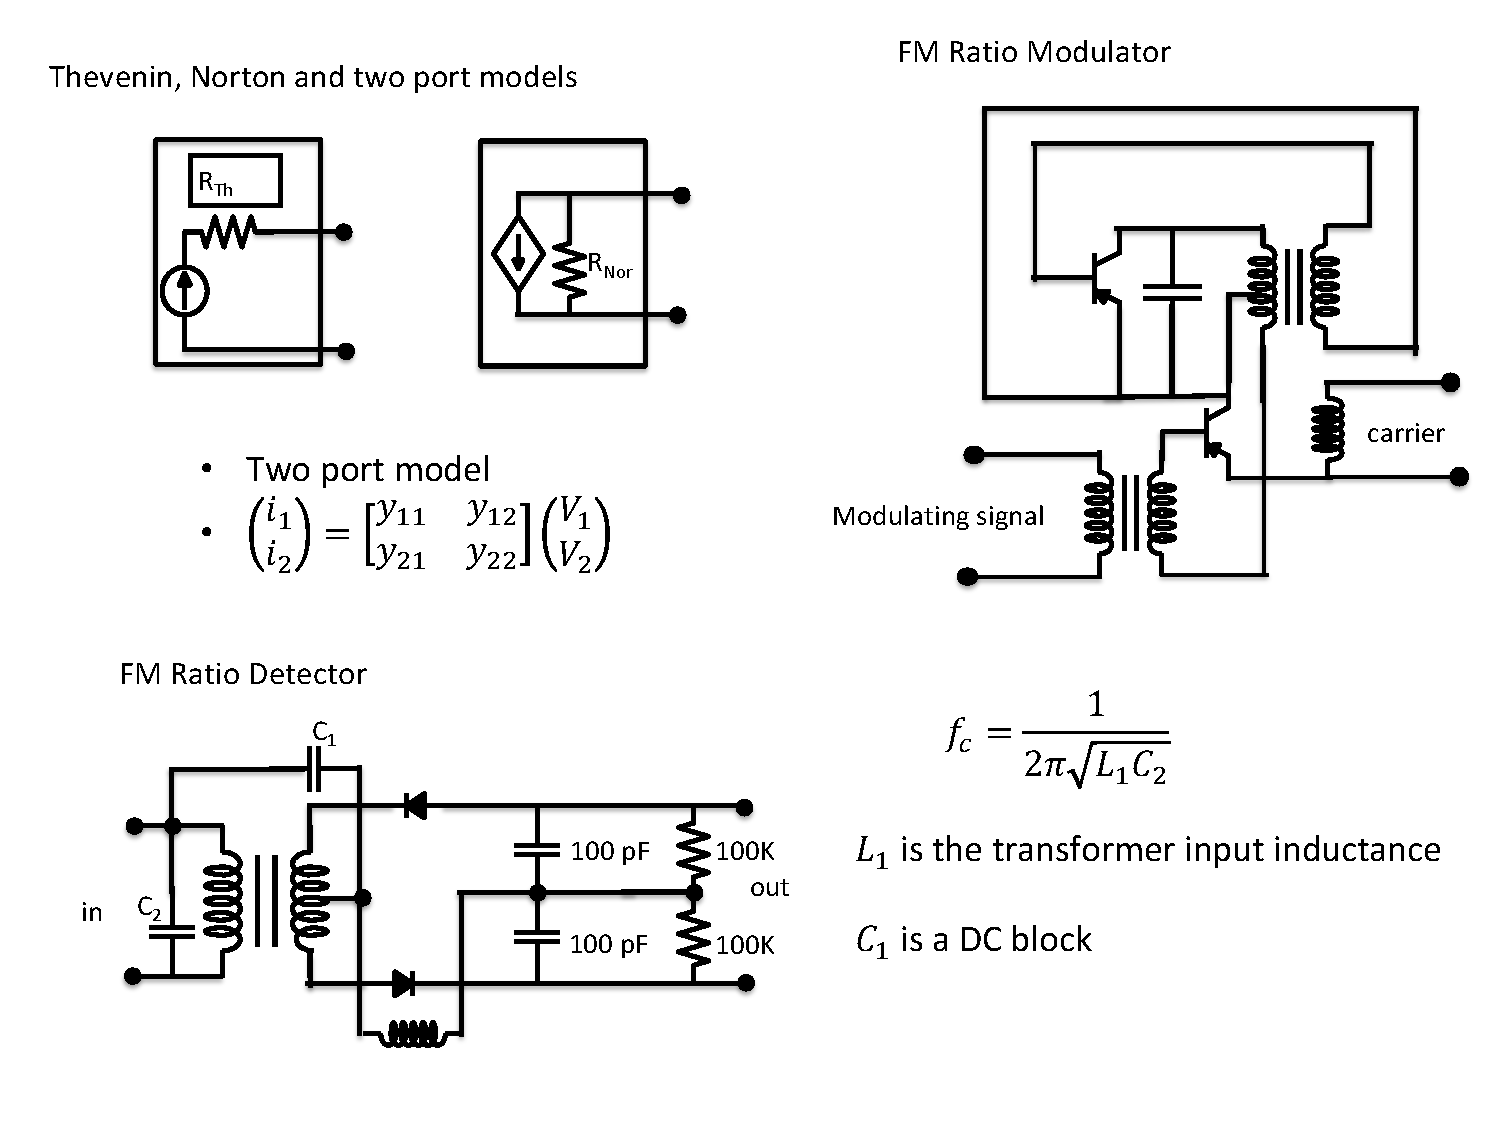
\includegraphics[width=0.8\textwidth,natwidth=642,natheight=610, height=80mm, width=88mm]{circuit16.pdf}
\end{figure}
\begin{figure} 
\center
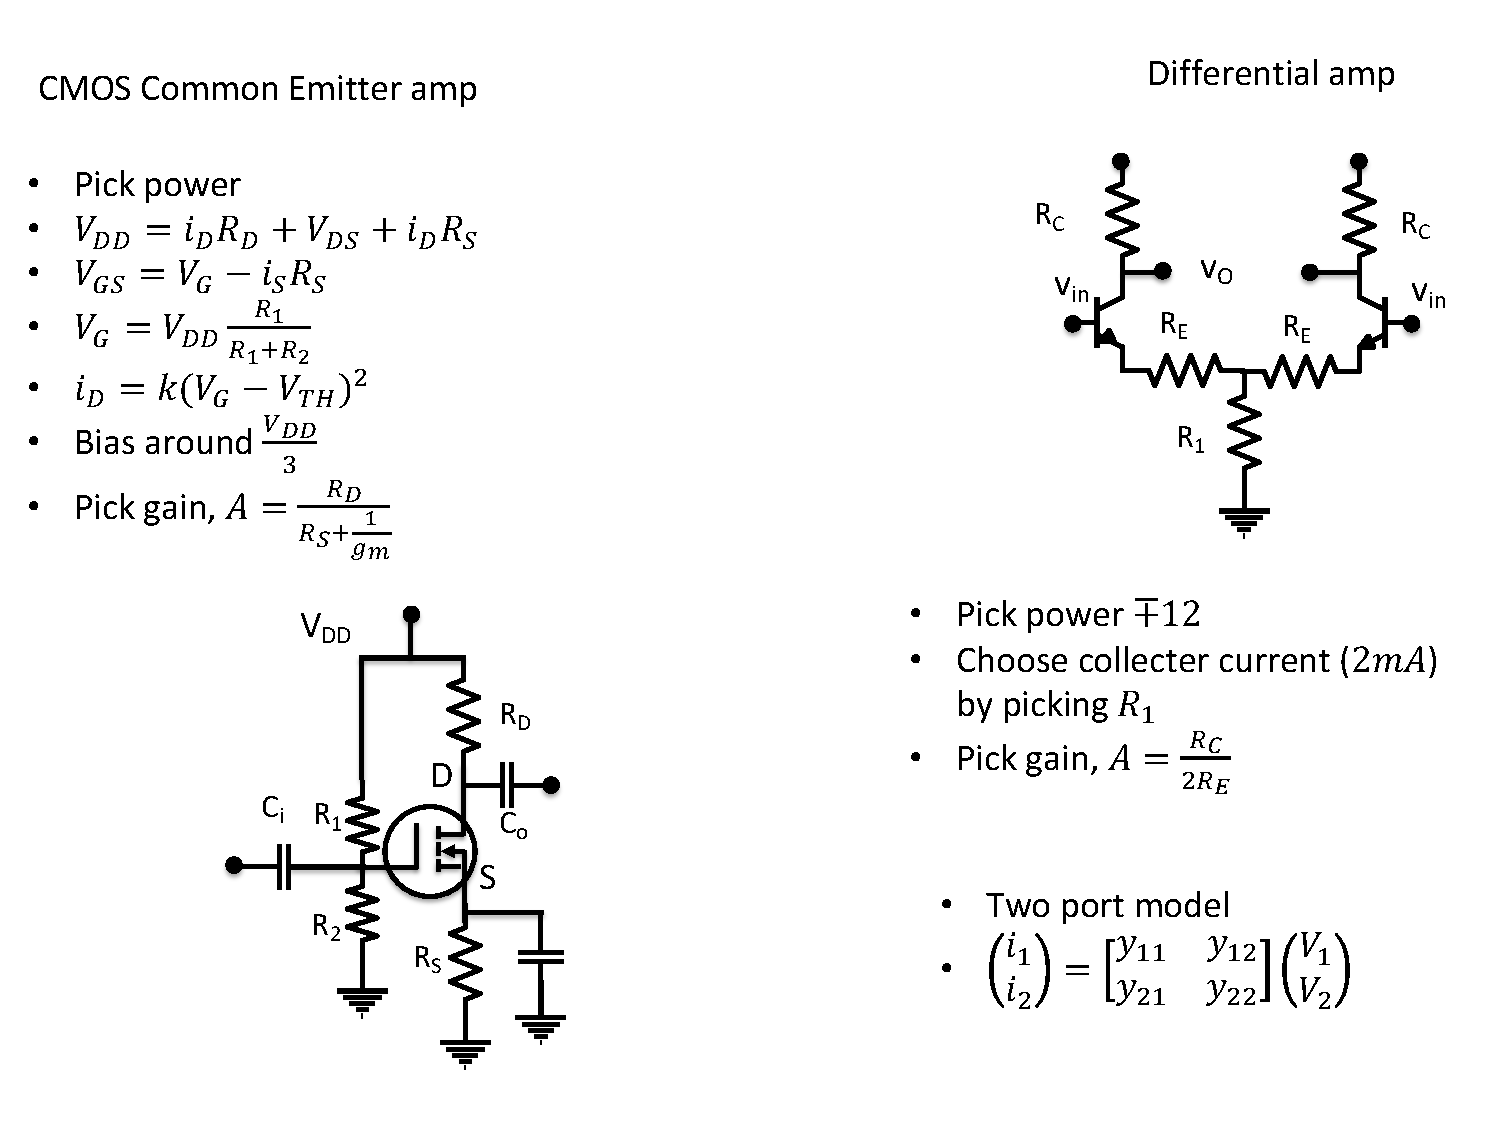
\includegraphics[width=0.8\textwidth,natwidth=642,natheight=610, height=80mm, width=88mm]{circuit17.pdf}
\end{figure}
\begin{figure} 
\center
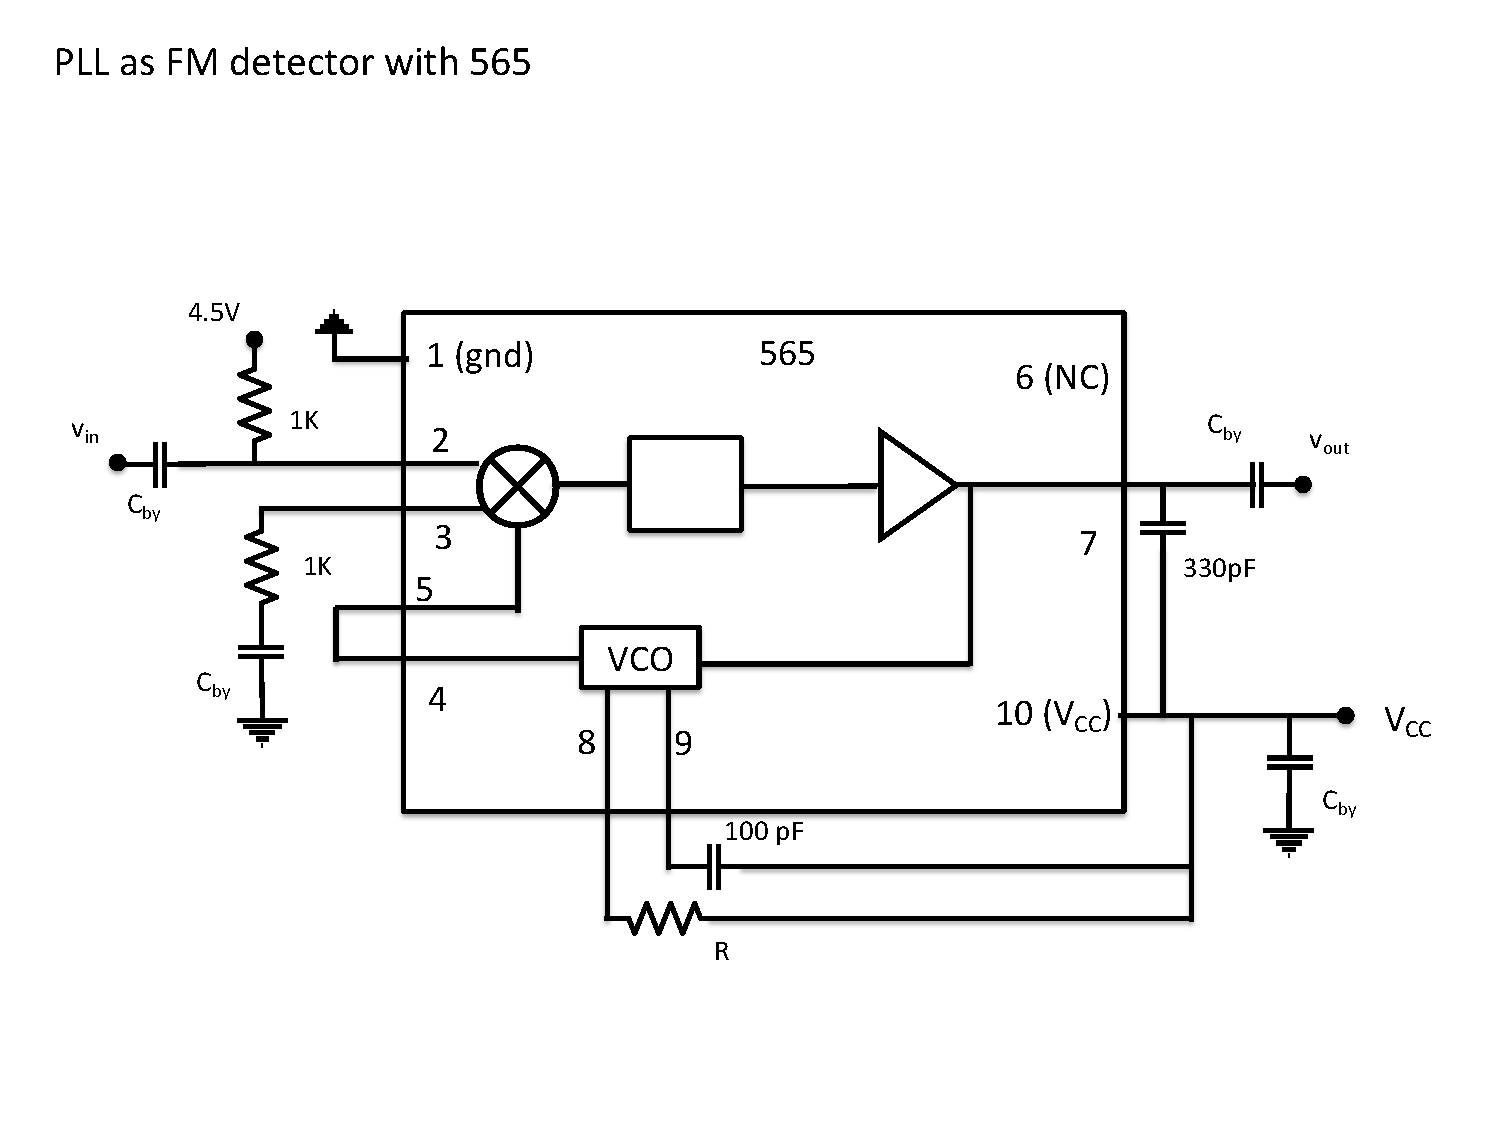
\includegraphics[width=0.8\textwidth,natwidth=642,natheight=610, height=80mm, width=88mm]{circuit18.pdf}
\end{figure}
\begin{figure} 
\center
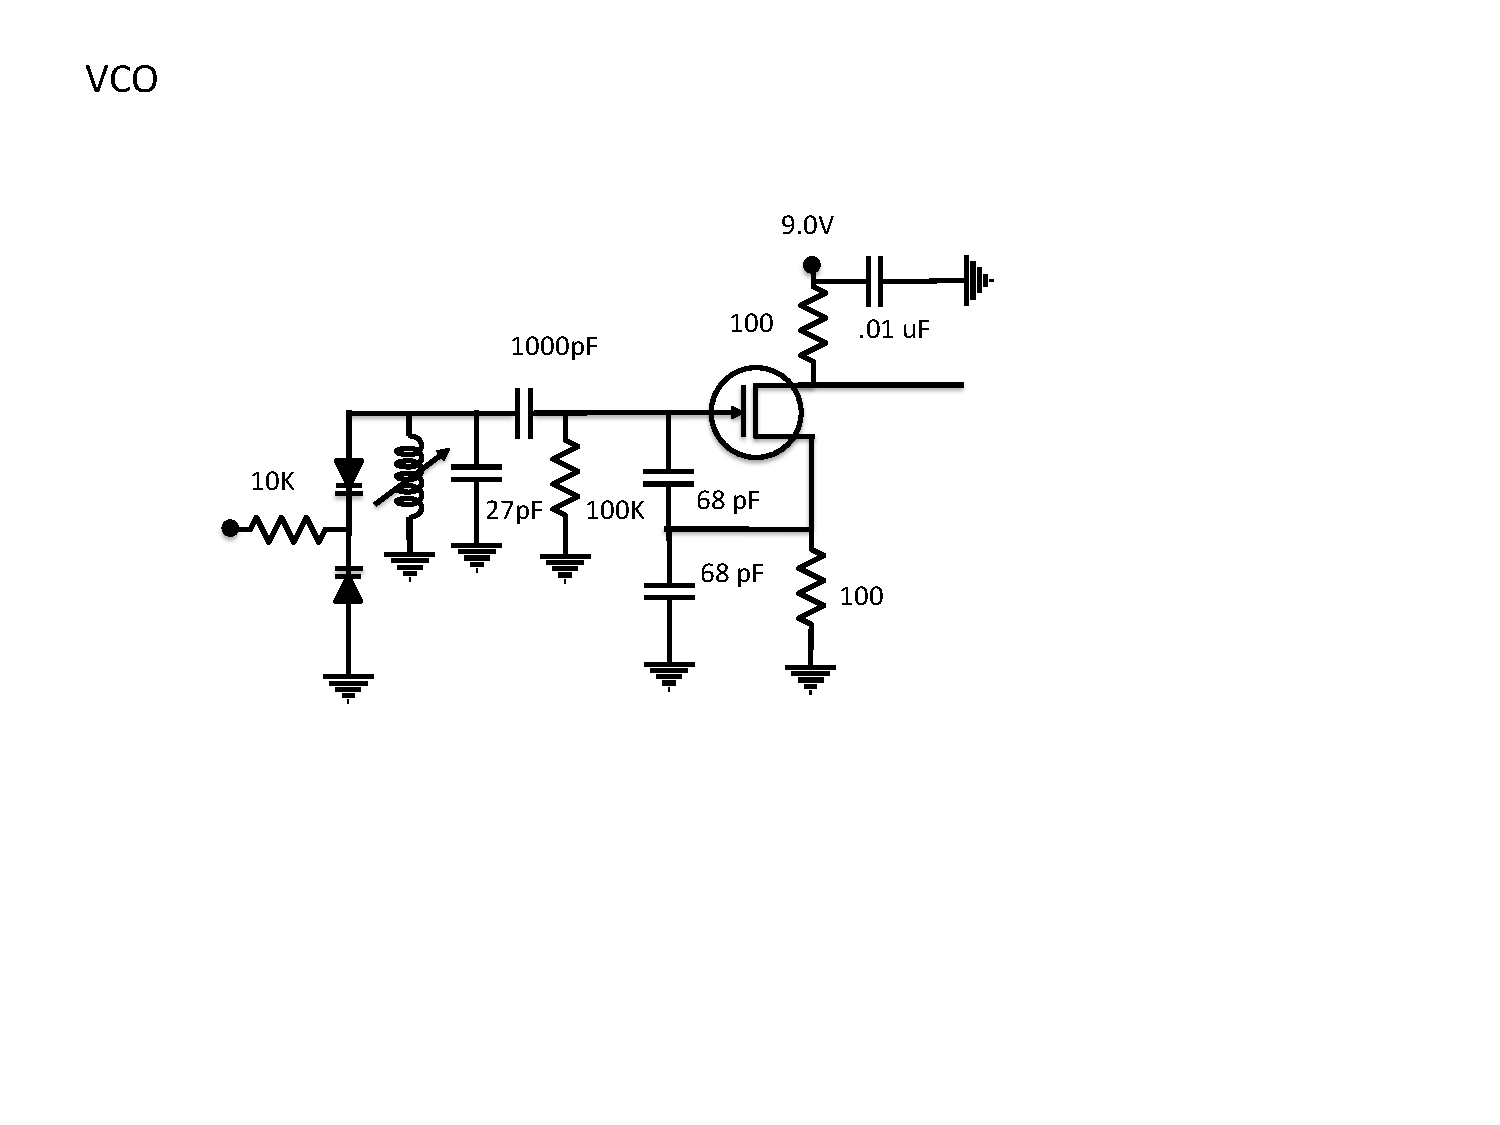
\includegraphics[width=0.8\textwidth,natwidth=642,natheight=610, height=80mm, width=88mm]{circuit19.pdf}
\end{figure}
\begin{figure} 
\center
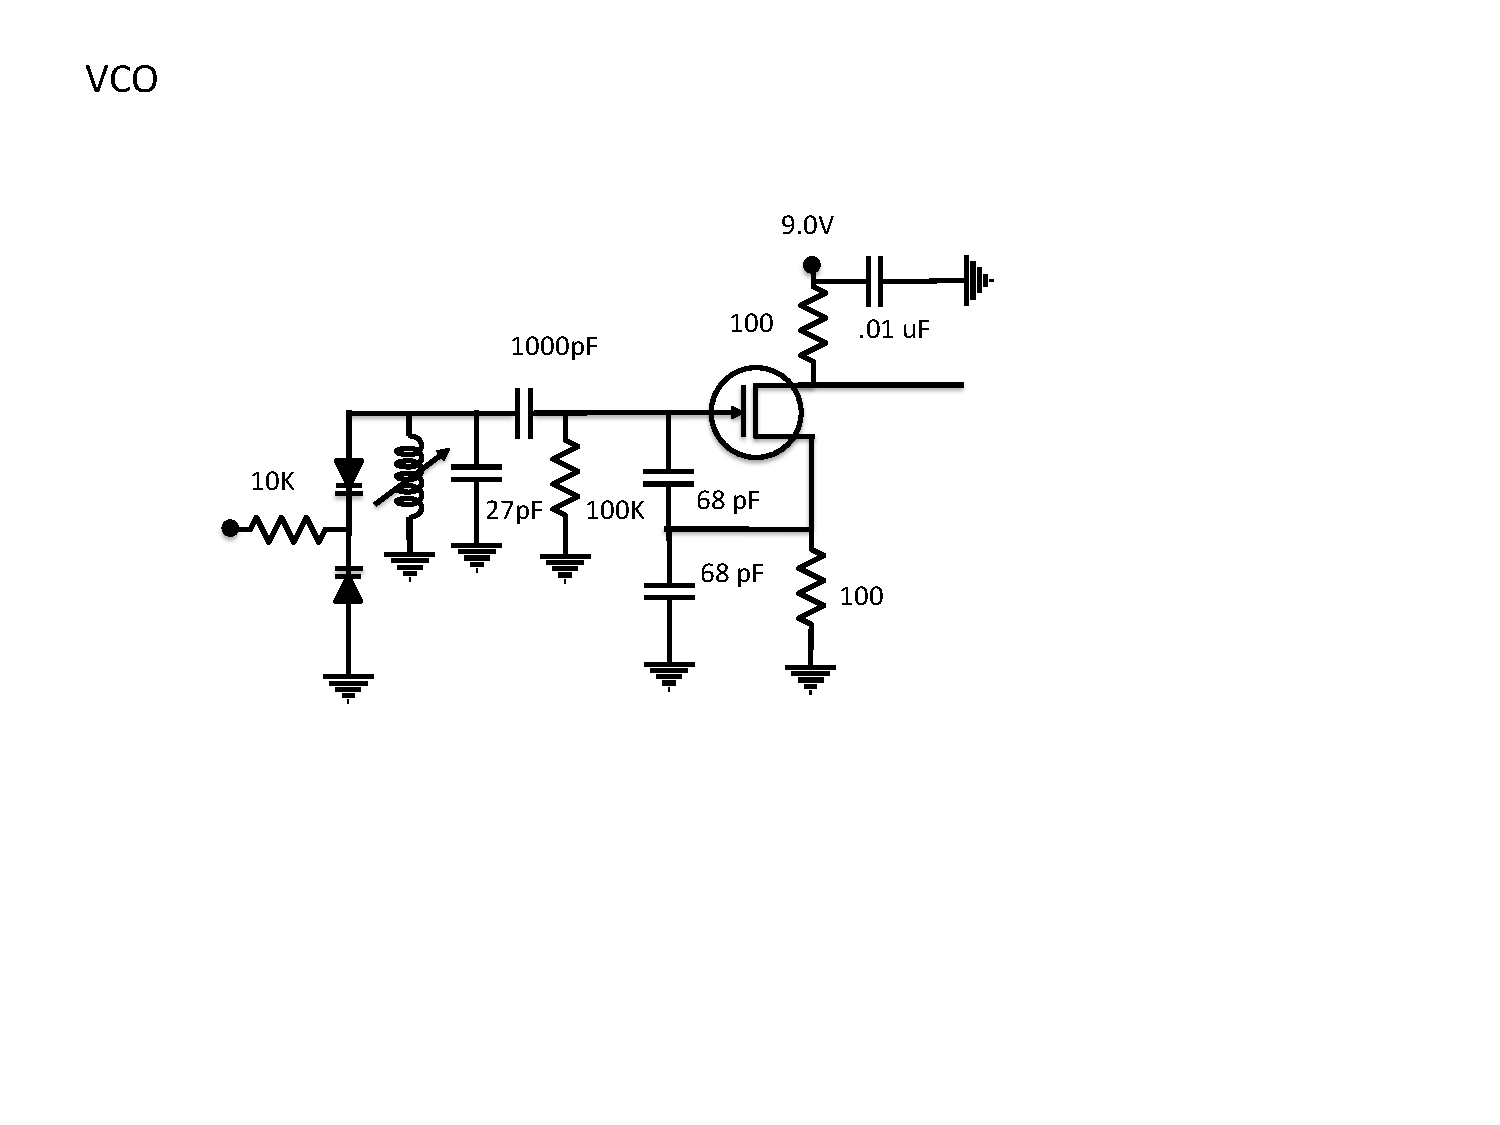
\includegraphics[width=0.8\textwidth,natwidth=642,natheight=610, height=80mm, width=88mm]{circuit21.pdf}
\end{figure}
\\
$\pi$\emph{-network:} $X_{C_1} = {\frac {R_{in}} {Q}}$,
$X_{L} = {\frac {QR_{in} + {\frac {R_{in}R_{out}} {X_{C_2}}}}
{Q^2+1}}$.
$R_{in} = 300$, $R_{out}= 50$, $F_C= \sqrt{7.7 \times 6.6}$,
$BW= 1.1$ MHz, $Q= {\frac {7.13}{1.1}}=6.48$,
$Q^2+1=43 > {\frac {300} {50}}$,
$X_{C_1} = 46.3 \Omega$,
$X_{C_2} = 20.1 \Omega$,
$X_{L} = 62.5 \Omega$.
\\
\\
{\bf Signal processing:} $h_n$ is impulse response to $\delta(0)$ at time step $n$.
$X( \omega ) = \sum_{n=-\infty}^{\infty} x(n) e^{-j \omega n}$; 
$x_n = {\frac 1 {2 \pi}} \int_{- \pi}^{\pi} X( \omega ) e^{j \omega n} d \omega$.
\emph{Frequency response:} $H( \omega ) = \sum h_n e^{-j \omega n}$.
$X(z)= \sum x_n z^{-n}$; $x_n = {\frac 1 {2 \pi j}} \int_S X(z) z^{n-1} dz$.
\\
\\
{\bf Real components:}
\emph{Real amp:}
$A= {\frac {I_C R_C} {\frac {kT} {q}}}$ and $I_C= {\frac {V_{BB}-V_{BE}} {R_E}}$,
$i_{c} \approx {\frac {v_{BB}-v_{BE}} {R_E}}, v_{BB}= v_{CC} {\frac {R_{B2}} {R_{B1}+R_{B2}}}$,
frequency response is ${\frac {1+j \omega C_1 R_2 }
{\sqrt{1+ \omega^2(r_1^2C_1^2+R_2^2C_2^2)+\omega^4(R_1C_1R_2C_2)^2}}}$.
\\
\emph{Air coil (solenoid):} $L=  {\frac {\mu n^2 A}{l}}$.
\\
\emph{Air coil:} $L(\mu H)= {\frac {d^2 n^2}{18d+40l}}$ (length in inches).
\\
\emph{Torodal coil, powdered iron:} $L(\mu H)= {\frac {A_L n^2}{10^3}}$ (length in inches).
\\
\emph{Torodal coil, ferrite:} $L(\mu H)= {\frac {A_L n^2}{10^6}}$ (length in inches). 
\\
\emph{Wire gauge
diameter:} 22 - 25 mil, 20 - 32 mil, 12 - 80 mil.  1 mil= .0254 mm.
\\
\\
{\bf Fourier representation:} $V(t)= {\frac {a_0}{2}} + \sum_{n=1}^{\infty} (
a_n cos(n \omega t) + b_n cos(n \omega t))$, 
$a_n= \int_{T/2}^{T/2} V(t) cos(n \omega t)$,
$b_n= \int_{T/2}^{T/2} V(t) sin(n \omega t)$.
\\
\\
{\bf Reflection on string:}
$ {\frac {\partial^2 \psi} {\partial t^2}} =
{\frac T {\rho}} {\frac {\partial^2 \psi} {\partial x^2}}$,
$v_{\phi}={\frac \omega k}$,
$v_{g}={\frac {d\omega} {dk}}$, $Z= {\sqrt {T \rho}}$.
\emph{Power:} $P(t)= F {\frac {\partial \psi} {\partial t}}$,
For travelling wave:
$P(t)= Z({\frac {\partial \psi} {\partial t}})^2$.
Consider a wave train on a string from the left ($L$) with a change
at $x=0$ of medium (i.e. a denser string) to a string on the right ($R$).
Dispersion caused by variation of wave velocity by frequency
relation $\omega= f(k)$.  Consider string of density $\mu_1$ connected
to string of density $\mu_2$ at $0$.  $f_1(x-{\frac {x} {v_1}}) + g(x+{\frac {x} {v_1}})
= f_2 (x- {\frac {x} {v_2}})$.  At $0$: $f_1(t)+g(t)=f_2(t)$ and
${\frac {f_1'(t)} {v_1}}-{\frac {g'(t)} {v_1}} = {\frac {f_2'(t)} {v_2}}$;
solve to get $g(t)= {\frac {v_2 - v_1} {v_2+v_1}} f_1(t)$ and
$f_2(t)= {\frac {2v_2} {v_2+v_1}} f_1(t)$.  \emph{Mach angle:}
$sin( \theta)= {\frac u v}$.
For perfect termination:
$F_{\small {term}} (\textnormal{``R on L''})= -
Z_L {\frac {\partial \psi_{inc}} {\partial t}} (0,t)$.
For excess force:
$F_{\small{term}} (\textnormal{``R on L''})= Z_L 
{\frac {\partial \psi_{ref}} {\partial t}} (0,t)$.
$-Z_L {\frac {\partial \psi_{inc}} {\partial t}} (0,t)+
Z_L {\frac {\partial \psi_{ref}} {\partial t}} (0,t) =
-Z_R ({\frac {\partial \psi_{inc}} {\partial t}} (0,t)+
{\frac {\partial \psi_{ref}} {\partial t}} (0,t))$.  So,
${\frac {\partial \psi_{ref}} {\partial t}} (0,t)=
{\frac {Z_L - Z_R} {Z_L + Z_R}}
{\frac {\partial \psi_{inc}} {\partial t}} (0,t)$.
$R= {\frac {Z_L - Z_R} {Z_L + Z_R}}$ is called the reflection coefficient.
\\
\\
{\bf Transmission boundary:} Let 
$v_I({\frac {x}{v_1}}-t), x < 0$,
$v_R({\frac {x}{v_1}}+t), x < 0$,
$v_T({\frac {x}{v_2}}-t), x > 0$ be respectively the incidence,
reflection and transmission voltages of a transmission line with boundary
at $x=0$.  Put $x=0$ to get 
$v_I(t)+v_R(t)=v_T(t)$. Expressing the current
flow at the boundary in terms of the voltages and the impedences ($Z_L, x<0$ and
$Z_R, x>0$), we get
${\frac {v_I(t)} {Z_L}}-{\frac {v_R(t)} {Z_L}}={\frac {v_T(t)} {Z_R}}$.
Solving we get, $v_R(t)= {\frac {Z_L-Z_R}{Z_L+Z_R}}v_I(t)$ and
$v_T(t)= {\frac {2Z_R}{Z_L+Z_R}}v_I(t)$.
\\
\\
{\bf Wave Transmission:}
\emph{String:} $v= {\sqrt {\frac F \mu}}$.
\emph{Fluid:} $v= {\sqrt {\frac B \rho}}$.
\emph{Solid:} $v= {\sqrt {\frac Y \rho}}$.
\emph{Adiabatic Gas:} $v= {\sqrt {\frac {\gamma p } \rho}}$.\\
\emph{Diffraction:} $I = I_0 ({\frac {sin({\frac {\beta} {2}})} {\frac {\beta}{2}}})^2$,
$\beta = {\frac {2 \pi a sin( \theta )} {\lambda}}$.
\\
Standing wave transmits no energy.
\\
\\
{\bf Early Quantum Mechanics:} $\Delta p \Delta x \geq {\frac {h} {4 \pi}}$,
$\hbar = {\frac {h}{2 \pi}}$,
$\lambda = {\frac {h}{p}}$,
$\nu = {\frac {E}{h}}$,
$p = {\frac { h k }{ 2 \pi }} = {\frac {p}{\lambda}}$,
$E = {\frac {h \omega}{2 \pi}}$,
$p_{av} = n k T$. \emph{Blackbody radiation:}
$E(\lambda , T ) = {\frac {8 \pi h c} {(\lambda^{5})}} (e^{{(h c)} /
{(\lambda k T )}}- 1)^{-1}$.  
\emph{Photoelectric Effect:} $hf= KE+ \phi$.
\emph{Bohr hydrogen atom:} $E_n = -{\frac {13.6 ev} {n^2}}$, $r_n=n^2a_0$,
$a_0= {\frac {h^2} {2 \pi k m c^2}}= .0529 nm$.
\emph{Time Independent Schrodinger:}
${\frac {d^2 \psi} {dt^2}}+{\frac {4 \pi m} {h}}(E-U(x)) \psi = 0$.
\emph{Schrodinger:}
${\frac {ih} {2 \pi}} {\frac {\partial \psi} {\partial t}} =
-{\frac {h^2} {8 \pi^2 m}} \nabla^2 \psi + V \psi$.
\\
\\
{\bf General Relativity:}
The \emph{proper interval} is $I(x,y,z,t)= c^2 t^2 - (x^2 + y^2 +z^2 )$, 
$I(x,y,z,t)=I(x',y',z',t')$.
$ds^{2}= g_{ij} dx^{i} dx^{j}$, $g_{ij} = g_{ji}$, $\delta \int {ds} = 0$.
The \emph{action} is $S= \int_{t_1}^{t_2} L(x, x', t) dt$, $\delta S=0 \rightarrow 
{\frac {\partial L} {\partial x}}- {\frac d {dt}} {\frac {\partial L} {\partial x'}}=0$.
$L(x,x',t)= {\frac {-m_0 c^2} {\sqrt {1-{\frac {v^2} {c^2}}}}} - q(\phi + v \cdot A)$.  
$R_{excess}= {\sqrt {\frac {A} {4 \pi}}} - r_{meas}= {\frac {G} {3 c^2}}M$,
${\frac {G} {3 c^2}}= 2.5 \times 10^{-29} {\frac {cm} {gm}}$.  From principle of
equivalence, $\omega= \omega_0 (1+ {\frac {gH} {c^2}})$ - doppler shift measured by 
Pound and Rebka. $\tau = {\frac L c}$ and $L = \int_0^t ||\dot{X}(t)|| dt$.
\emph{Equation of motion:} ${\frac {d^2 X} {{d \tau}^2}} = - {{\Gamma}^i}_{kl}
{\frac {d X^k} {d \tau}} {\frac {d X^l} {d \tau}}$; this corresponds to Newtonian
$\ddot{x}^{\alpha} = - {\frac {\partial \Phi} {\partial x^{\alpha}}}$.  
\\
\\
{\bf Maxwell's equations (CGS):}
$\nabla \cdot {\vec j} = - {\frac {\partial \rho} {\partial t}}$,
$\nabla \cdot {\vec E} =  4 \pi {\rho}$, 
$\nabla \times {\vec E} = - {\frac 1 c} {\frac {\partial {\vec B}}{\partial t}}$,
$\nabla \cdot {\vec B} = 0$,
$\nabla \times {\vec B} = {\frac {4 \pi} c} {\vec j} +
{\frac 1 c} {\frac {\partial {\vec E}} {\partial t}}$.
\begin{figure} [h]
\begin{center}
\begin{tabular} {|l|}
\hline
{\bf CGS Units:} $k=1$.  $F= q(E + {\frac v c} \times B)$.  
$1$ statvolt$=$ $300$ volts\\
$1$ statvolt/cm $=$ $3 \times 10^4$ volts/m\\
$1$ T $=$ $10^4$ G\\
$1$ C $=$ $3 \times 10^9$ esu\\
$1$ ohm $=$ $1.139 \times 10^{-12}$ sec/cm\\
$1$ weber $=$ $10^{8}$ G-cm\\
$1$ J $=$ $10^{7}$ ergs\\
$1$ N $=$ $10^{5}$ dynes\\
\hline
\end{tabular}
\end{center}
\end{figure}

\begin{figure} [h]
\begin{center}
\begin{tabular} {|r|r|r|r|r|r|}
\hline
{\bf System} & $\epsilon_0$ & $\mu_0$ & ${\vec D}, {\vec H}$ & {\bf Maxwell's equations} & {\bf Lorentz Force} \\
\hline
 & & & ${\vec D}= {\vec E} + 4 \pi {\vec P}$ & 
$\nabla \cdot {\vec D}= 4 \pi \rho$ & \\
 & & & & 
$\nabla \times {\vec H} = {\frac {4 \pi {\vec j}} {c}} + {\frac 1 c} {\frac {\partial {\vec D}} {\partial t}}$ & $q ({\vec E} + {\frac {\vec v} {c}} \times {\vec B})$ \\
Gaussian & $1$ & $1$ & & 
$\nabla \cdot {\vec B} = 0$ & \\
 & & & ${\vec H}= {\vec B} - 4 \pi {\vec M}$ & 
$\nabla \times {\vec E} + {\frac 1 c} {\frac {\partial {\vec B}} {\partial t}}= 0$ & \\
\hline
 & & & ${\vec D}= \epsilon_0 {\vec E} + {\vec P}$ & 
$\nabla \cdot {\vec D}= \rho$ & \\
 & & & &
$\nabla \times {\vec H} = {\vec j} + {\frac {\partial {\vec D}} {\partial t}}$ & 
$q( {\vec E} + {\vec v} \times {\vec B} )$ \\
MKS & ${\frac {10^{-9}} {36 \pi}}$ & $4 \pi \times 10^{-7}$ & & 
$\nabla \cdot {\vec B} = 0$ & \\
 & & & ${\vec H}= {\frac {\vec B} {\mu_0}} - {\vec M}$ & 
$\nabla \times {\vec E} + {\frac {\partial {\vec B}} {\partial t}}= 0$ & \\
\hline
\end{tabular}
\end{center}
\caption{Maxwell's Equations in MKS and CGS}
\end{figure}
\section{Physical Constants}
{\bf Conversion factors:}
$1 \; in= 2.54 \; cm$.
$1 \; meter= 39.370 \; in$.
$1 \; AU= 1.496 \times 10^{11}\; m$.
$1 \; lb= 4.448 \; N$.
$1 \; Pa= 1 \; {\frac {N} {m^2}}$.
$1 \; Atm= 1.013 \times 10^{5}\; Pa$.
$1 \; hp= 745.7 \; W$.
$1 \; J= 10^{7}\; erg$.
$1 \; ev= 1.602 \times 10^{-19}\; J$.
$1 \; BTU= 1055 \; J$.
$1 \; cal= 4.186\; J$.
$1 \; L= 1000 \; cm^3$.
$1 \; Gal= 3.785 \times 10^{-3}\; m^3$.
$1 \; kg = 2.2046 \; lbs$, $1 \; fluid-oz = 0.0338 \; ml$, 
$1 \; gal = 3.3785 \; liters$.
\\
\\
{\bf Atomic constants:} $M_{e} = .510998 \textnormal{Mev}= 9.10939 \times 10^{-31} kg$,
$M_{p} = 938.256 \textnormal{Mev} (=1836 M_{e})= 1.67262 \times 10^{-27}kg$,
$M_{n} = 939.55 \textnormal{Mev} = 1.67493 \times 10^{-27} kg$,
$\sigma_{SB} = 5.67 \times 10^{-8} W m^{-2} K^{-4}$,
$1 ev = 1.6 \times 10^{-12} erg = 1.6 \times 10^{-19} J$,
$1 curie = 3.7 \times 10^{12} decays$, $c_{s} = 3.32 \times 10^{4} cm/s$,
$1 kg TNT= 4.2 MJ$,
$1A = 10^{-8} cm$.  \emph{HDNA:} 2,900,000 kilobases.
\\
\\
{\bf Astronomical constants:} $H_{0} = 100 \textnormal{km{(s-Mpc)}}^{-1}$,
$1 \textnormal{ pc}= 3.26 l-y$,
$10^{80} \textnormal {nucleons}$, $10^{28} \textnormal{cm-diam}$, $10^{11} \textnormal{galaxies}$.
\\
\emph{Milky Way:} $\epsilon_{\small{ecliptic/MW}}= 62.5$,
$1.6 \times 10^{11} \textnormal{stars}$, $10^{23} \textnormal{cm-diam}$, $8 \times 10^{44} 
\textnormal{gm}.$ \\ \emph{Sun:} $E_{\small{sun}} = 4 \times 10^{33} 
\textnormal{ergs/sec}$,
$R_{\small{Su}n}= 3.5 \times 10^{10} cm$, $1.99 \times 10^{33} \textnormal{gm}$,
$\lambda_{\small{sun}} = 30 days.$ \\ \emph{Earth:} $\epsilon_{earth} =23.5$,
50\% clouds, $R_{
\small{moon}} = 2160 mi$, $\epsilon_{\small{moon}} = 5$, 
$\lambda_{\small{sider}} =  27d7h43m12s$, $\lambda_{
\small{synod}} = 29d12h44m3s$, $D_{moon}= 363,300 - 405,500 km$.
$RA_{\small{Greenwich}}  (1986.0): 6.6245$,
$ 0 \; Jan \; 1986= 2,446,430.5JD$.
\\
\\
{\bf Geological:}
For seismic wave,
$v_P= {\sqrt {\frac {(k+{\frac 4 3} \mu)} {\rho}}}$,
$v_S= {\sqrt {\frac {\mu} {\rho}}}$. \\
$\mu_{granite}= 1.6 \times 10^{10} dynes/cm$,
$k_{granite}= 27 \times 10^{10} dynes/cm$,
$k_{water}= 2.0 \times 10^{10} dynes/cm$,
$\mu_{water}= 0$.
$v_{P-granite}= 5.5 km/sec$,
$v_{S-granite}= 3.0 km/sec$,
$v_{P-water}= 1.5 km/sec$,
$v_{S-water}= 0$.
\\
\\
{\bf Materials: }
\emph{Young's Modulus:} ${\frac F A} = Y {\frac {\Delta L} {L}}$.\\
\emph{Bulk Modulus:} ${\frac F A} = B {\frac {\Delta V} {V}}$.\\
\emph{Shear Modulus:} ${\frac F A} = G {\frac {\Delta x} {L}}$.\\
\emph{Viscosity:} $\eta = {\frac {\frac F A}  {\frac {\Delta v} {h}}}$.\\
\emph{Surface tension:} $\gamma_{H_2O}= 72.8 \times 10^{-4} N/m$.\\
\emph{Reynold's number:} $Re = {\frac {\rho {\overline v} L} {\eta}}$;
turbulent flow if $Re>4000$, laminar if $Re<2000$.\\
Dry (static, sliding) Friction:  Steel (.78,.42), Teflon; (.04,-).\\
\emph{Expansion:}
$\alpha_{l} = l^{-1} {\frac {\partial l} {\partial t}} \times 10^{6}$,
C: (Al, 24), (Cu, 17), (Granite, 8.3), (Ice, 50), (Fe, 12), (Water, 207).\\
\emph{Heat Capacity:}
$c_{v} =  m^{-1} {\frac {\partial Q } {\partial T}}:$ [${\frac {J}{mol-\thinspace^oK}}$]
(He, 12.5), ($O_{2}$, 21.1), ($N_{2}$, 20.6),
($C_{2}H_{6}$ , 39.3), MFP $N_{2}= 10^{-5}$ cm,
$C_{v,solid} = 3 R$.\\
$c_{v,air} \approx 700 {\frac {J} {kg-\thinspace^oK}}$.
\emph{Melting/Boiling:}
MP/BP (K): Au, 1336, 3081; $O_{2}$, 54, 90; Cu, 1356, 2839.\\
\emph{Heat Conduction:}
$Q' = - \kappa A  {\frac {\partial T} {\partial l}} W{(cmK)^{-1}}: $
(Cu, 4), (Fe, 0.80), (Si, 1.5), ($H_{2}$,.00024-.0018),
(Rock, 2.8 kc/mhK).\\
\emph{Dielectric:}
$\epsilon = K \epsilon_{0}$: (Glass, 6.7), (Water, 78), (Nylon, 3.6).
\\
\emph{Resistivity:}
$R= \rho {\frac {L}{A}}  \times 10^{-8}$: (Ag, 1.4), (Cu, 1.7), (Al, 2.8),
(Fe, 9.8).
\\
\emph{Density:}
$\rho / \rho_{water}$: Al, 2.7; Cu, 8.9; Rock, 5.5; Au, 19; Fe, 7.8; Gas, .68 ($g/cm^3$);
air, .0012; wood, .75.  \\
\emph{Moduli:}
$B= {\frac {\Delta P} {\frac {\Delta V} {V}}}:$ Al, 70;
Cu, 140; Fe, 100; Water, 2.2 ($GPa$).  \\
$Y= {\frac {\frac {\Delta F}{A}} {\frac {\Delta l}{l}}} \times
10^{12} dy/cm^{2}$: Al, 70; Cu, 110; Fe, 190.  \\
$M_{s} = {\frac {\frac {\Delta F} {A}} {\frac {\Delta x} {l}}}:$
Al, 30; Cu, 42; Fe, 100.\\
Energy content of one gallon of heating oil: $140,000 kJ/gallon$.
\\
\\
{\bf Air:} 28.96 m-w, $c_{p}$ = 1005 J/kg-K, $c_{v} = 718 J/kg-K$.
$1\; atm= 1.013 \times 10^{5} Pa$, $Pa= 10^{6} dyne/cm^{2}= 1N/m^2=760 mm-Hg$.
$\rho: 1.293 mg/cm^{3}$, $\kappa :  2.4 \times 10^{-2} W/m-K$, $visc@20: .00018 g/cm-s.$
\\
\\
{\bf Water:} 273.15K, 18 m-w, 540 cal/gm (vaporization), 80 cal/gm (fusion),
$\rho_{ice} = 917 kg / m^{3}$,
$\rho_{water} = 1 g / cm^{3}$,
$\kappa:  .19 W/m-K, visc@20: .01gm/cm-s, ST: @20: 73d/cm.$  Specific
heat of water: $1 cal/K-gm= 4.186 J/K-gm$.
\\
\\
{\bf Sound:}
\emph{Sound strength:} $g= 10 log({\frac {I} {I_0}})$ in db.  $I_0 = 10^{-12}
W/m^2$. Normal Conversation: 60 db, Jet: 130 db.
\emph{Speed of Sound:}
$\approx 330 m/s$ at normal conditions,
$v_{av} = {\sqrt { {3 k T } / m }}$.
\\
\\
\begin{figure} [h]
\begin{center}
\begin{tabular} {|lllll|lllll|}
\hline
{\bf Name} & {\bf RA} & {\bf Dec} & {\bf Vmag} & {\bf Dist} & {\bf Name} & {\bf RA} & {\bf Dec} & {\bf Vmag} & {\bf Dist} \\
\hline
Polaris & 01 23 & 88 46 & 2.06 & 200 & Mizar & 13 20 & 55 27 & 2.12 & 26 \\
\hline
Aldeberan & 04 30 & 16 19 & .8 & 21 & Capella & 05 09 & 45 54 & .09 & 14 \\
\hline
Rigel & 05 10 & -08 19 & .11 & 270 & Bellatrix & 05 20 & 06 16 & 1.63 & 140 \\
\hline
Betelgeuse & 05 50 & 07 23 & .4 & 180 & Sirius & 06 41 & -16 35 & -1.44 & 2.7 \\
\hline
Canopus & 06 22 & -52 38 & -.72 & ? & Castor & 07 28 & 32 06 & 1.56 & 14 \\
\hline
Procyon & 07 34 & 05 29 & .36 & 3.5 & Pollux & 07 39 & 28 16 & 1.15 & 10.7 \\
\hline
Regulus & 10 03 & 12 27 & 1.34 & 26 & Merak & 10 56 & 56 55 & 2.36 & 23 \\
\hline
Spica & 13 20 & -10 38 & .97 & 65 & Arcturus & 14 11 & 19 42 & -.05 & 11 \\
\hline
Antares & 16 23 & -26 13 & .94 & 130 & Vega & 18 34 & 38 41 & .03 & 8.1 \\
\hline
Altair & 19 46 & 08 36 & .77 & 4.9 & Deneb & 20 38 & 44 55 & 1.25 & 500\\
\hline
\end{tabular}
\end{center}
\caption{Stars}
\end{figure}
\begin{figure} [h]
\begin{center}
\begin{tabular} {|lllllllllll|}
\hline
{\bf Planet} & $\mathbf {D_{av}(km \times 10^6)}$ & $\mathbf {\lambda(rev)}$ & 
$\mathbf {e}$ & $\mathbf {i}$  & $\mathbf {L_{node}}$ & $\mathbf {L_{Per}}$ &
$\mathbf {P_{epoch}}$ & {\bf M(gm)} & {\bf R(km)} & {\bf Rot}\\
\hline
Mercury & 57.9 & 87.97d & .2 & 7 & 47.9 & 76.8 & 222.6 & 3.3e26 & 2439 & 58.7d\\
\hline
Venus & 108.2 & 224.7d & .007 & 3.4 & 76.3 & 131.0 & 174.3 & 4.9e27 & 6050 & 243d\\
\hline
Earth & 149.6 & 365.26 & .017 & 0 & 0 & 102.3 & 100.2 & 6e27 & 6378 & 23h56m\\
\hline
Mars & 227.9 & 686.98 & .093 & 1.8 & 49.2 & 335.3 & 258.8 & 6.4e26 & 3394 & 24h37m\\
\hline
Jupiter & 778.3 & 11.8yr & .048 & 1.3 & 100.0 & 13,7 & 259.8 & 1.9e30 & 71880 & 9.8h\\
\hline
Saturn & 1427.0 & 29.46 & .056 & 2.5 & 113.3 & 92.3 & 280.7 & 5.7e29 & 60400 & 10.66h\\
\hline
Uranus & 2869 & 84 & .047 & .8 & 73.8 & 170.0 & 141.3 & 8.8e28  & 23540 & 17.24h\\
\hline
Neptune & 4496 & 164.79 & .009 & 1.8 & 131.3 & 44.3 & 216.9 & 1e29 & 24600 & 16h\\
\hline
Pluto & 5900 & 247.7 & .250 & 17.2 & 109.9 & 224.2 & 181.6 & - & - & - \\
\hline
\end{tabular}
\end{center}
\caption{Planetary data - Epoch: 1960 Jan 1.5UT,
Orbit:  $a = b {\sqrt {1 - e^{2}}}$.}
\end{figure}
\begin{figure} [h]
\begin{center}
\begin{tabular} {|lrr|lrr|lrr|}
\hline
{\bf Place} & {\bf Lat} & {\bf Long} & {\bf Place} & {\bf Lat} & {\bf Long} & {\bf Place} & {\bf Lat} & {\bf Long} \\
\hline
Beijing & 40.1 & 116.33 & SF & 37.45 & -122.33 & NY & 41.44 & -73.8 \\
\hline
Boston & 42.35 & -71.05  & Chicago & 41.87 & -87.63 & Dallas & 32.78 & -96.78  \\
\hline
Madison, Wi & 43.07 & -89.38 & Santa Fe & 35.68 & -105.93  & Seattle & 47.61 & -122.33 \\
\hline
Tucson & 32.22 & -110.97  & DC & 38.88 & -77.0 & Denver & 39.75 & -104.99  \\
\hline
Atlanta & 33.75 & -84.39 & London & 51.5 & 0.0 & Paris & 48.83 & 2.3 \\
\hline
Berlin & 52.5 & 13.42  & Rome & 41.88 & 12.5 & Moscow & 55.75 & 37.7 \\
\hline
Athens & 37.97 & 23.75 & Jerusalem & 31.75 & 35.22  & Tokyo & 35.75 & 139.75 \\
\hline
Sidney & -33.87 & 151.2 & MKea & 19.826 & -155.47 & CTlo & -70.82 & -30.17  \\
\hline
New Orleans & 29.93 & -90.07 & Redmond,OR & 44.27 & -121.15 & Portland & 45.52 & -122.68 \\
\hline
LA, CA & 34.05 & -118.24  & San Diego & 32.7 & -117.15 & Orlando & 28.52 & -81.38  \\
\hline
Milan & 45.45 & 9.28 & Amsterdam & 52.3 & 4.77  & Auckland & -36.92 & 138.58 \\
\hline
Bombay & 18.93 & 74.58  & Delhi & 28.67 & 77.23 & Perth & -31.93 & -115.83  \\
\hline
Toronto & 43.65 & -79.38 & Bagdad & 33.3 & 44.43 & Cairo & 30.03 & 31.35 \\
\hline
\end{tabular}
\end{center}
\caption{Places on Earth}
\end{figure}
\\
\\
{\bf Stellar Evolution} ($'$: means differentiate wrt $r$):
$P'= - \rho {\frac {G M(r)} {r^{2}}}$, $M'= 4 \pi r^{2}\rho$,
$L'= 4 \pi r^{2} \epsilon$,\\
$L'= {\frac {(-3 \chi \rho)}  {(4 a c T^{3} (4 \pi r^{2})) }}$ (rad),
$L'= (1 - \gamma^{-1}) T  \rho^{-1} P'$ (conv),
$P=RT {\frac {\rho} {\mu}}$,
$\chi = C \rho T^{-3.5}$, $\alpha = {\frac {10^{6}} {T^{1/3}}}$.
\\
\\
{\bf Optics:} $n_{glass}= 1.52$, $n_{water}= 1.33$, $n_{diamond}=2.42$.  
\emph{Lensmaker's law (air to glass, one surface):}
${\frac 1 s} + {\frac n {s'}}= {\frac 1 f}$.
\emph{Lensmaker's law (double surface):}
${\frac {n_1} s} + {\frac {n_2} {s'}}= {\frac 1 f}$,
${\frac 1 f}= (n_2 - n_1 ){\frac 1 {R_1}}-{\frac 1 {R_2}}$.
${\frac {h_i} {h_o}}= {\frac {d_i} {f}}={\frac {f} {d_o}}$.
\emph{Resolving Power:}  4.54/$D_{\small {inches}}$ arc-seconds,
$f_{\small{ratio}} = {\frac {L_{\small {focus}}}  {R_{\small {diameter}}}}$,
$3 \leq f_{\small {ratio}} \leq 6$,
$Mag= {\frac {L_{\small {focus-objective}}} {L_{\small {focus-eyepiece}}}}.$
\emph{Lens:}  Original object $PA$ of height $y$ with ray intersecting focus at $S$ hitting 
lens at $U$ to
(inverted) image $BR$ of height
$y'$.  Similarly, ray from $P$ parallel to axis hitting lens at $Q$ intersecting
focus at $T$.  $x$ is distance from $A$ to $S$ and $x'$ from $T$ to $B$; finally, $f$ is the
distance from the focus to the lens.
$ {\frac {PA}{AS}}= {\frac {QU}{PQ}} $ and
$ {\frac {BR}{TB}}= {\frac {QU}{UR}} $.  Thus,
$ {\frac {y}{x}}= {\frac {y+y'}{x+f}} $ and
$ {\frac {y'}{x'}}= {\frac {y+y'}{x'+f}} $.  $f^2 = x x'$.  
\emph{Magnification:}
${\frac {y}{y'}}= {\frac {x'} {f}}= {\frac {f}{x}}$.
\\
\\
{\bf Chemical bonds:}
\emph{Covalent:} 80-200  kcal/mole (C=C is 200), 
\emph{Ionic:} 4-7 kcal/mole,
\emph{Hydrogen:} 5kcal/mole, 
\emph{VanderWaal:} $<1kcal/mole$ (methane).
\emph{Thermal:} ~.6 kcal/mole.
Acid added to $H_{2}O$ increases $H^{+}, pH= -log[H^+]$, acid $< 7$.
\\
\\
{\bf Fluids:}  $P + \phi + {\frac {1}{2}} \rho v^{2} = const$,
$\nabla \rho v = - \rho '$,
$\nabla v = 0$,
$\nabla \times v=0.$\\
\\
{\bf Interference:} $R=A[
cos(\omega t) + cos(\omega t + \phi) + \ldots + cos(\omega t + (n-1)\phi)]$.
$A_R= A {\frac {sin({\frac {n \phi} {2}})} {sin({\frac {\phi} {2}})}}$.
$I= I_0 
{\frac {sin^2({\frac {n \phi} {2}})} {sin^2({\frac {\phi} {2}})}
}$.  For 
$f(t)= A_1 e^{i \omega_1 t} + A_2 e^{i \omega_2 t}$,
$I= A_1^2 + A_2^2 + 2 cos((\omega_1 - \omega_2)t)$.  Group velocity and modulation.
\\
\\
{\bf Damped and driven simple harmonic oscillators:}  
Solution of $m\ddot{x} +kx=0$ 
is $Acos(\omega t)+Bsin(\omega t)$ where $\omega= {\sqrt {\frac k m}}$.
Solution of $m\ddot{x} +b \dot{x} +kx=0$
is $e^{- \omega_0 t} (Acos(\omega t)+Bsin(\omega t))$ where 
$\omega= {\frac {\sqrt {b^2-4 k m}} {2m}}$ and
$\omega_0= {\frac b {2m}}$.
Solution of $m\ddot{x} +b \dot{x} +kx= F cos(\gamma t)$ is
$e^{- \omega_0 t} (Acos(\omega t)+Bsin(\omega t)) +
\alpha cos(\gamma t)+ \beta sin (\gamma t)$ where 
$\alpha= F{\frac {k- m \gamma^2} {(b \gamma)^2 + (k - m \gamma^2)^2}}$ and
$\beta= F{\frac {b \gamma} {(b \gamma)^2 + (k - m \gamma^2)^2}}$.
\\
\\
{\bf Spectrum:}  
30cps audio 30K 500K AM 1500K 3M HF 30M 88M FM VHF 210M 400M UHF 800M 1.5G 
$H_{2}$ S-band 3G 7600A IR 6300 Visible 3900A UV 100A X-ray .1A gamma
67 Mev. 
\\
{\bf IEEE:} HF ($.003 - .03$ G), VHF ($.03 - .3$ G), UHF ($.3 - 1$ G), L ($1 - 2$ G),
S ($2 - .4$ G), C ( $4 - 8$ G), X ( $8 - 12$ G),
Ku ($12 - 18$ G), K ($18 - .27$ G), Ka ($27  - 40$ G),
V ($40 - 75$ G), W ($75 - 110$ G), G ($110 - 300$ G).
\\
Red: 650nm, Yellow: 580 nm, Green: 500nm, Blue: 475nm, Violet: 400Nm.  
\\
\\
{\bf Fris and dB:} dBm- relative to 1 mW, dBc - relative to carrier.
$P_r = {\frac { P_t G_t G_r \lambda^2} { (4 \pi)^2 d^2}}$. 120 dB at 433MHz,
$d= 2km$.
\\
\\
{\bf Radar range equation:} $R^4= {\frac {P_{tx} G^2 \sigma \lambda^2}
{(4 \pi)^3 P_{rx, min)}} }$, $P_{rx, min} = k T B F (SNR)_{min}$.
\\
\\
{\bf Middle C:}  256Hz. Octave has 12 notes in uniformly divided log scale.
Octave is factor of 2.
\\
\\
{\bf Central Forces:} $\vec{a}(r)=f(r) \hat{r}$.  
$(\ddot{r}-r{\dot{\theta}}^2)=f(r)$ and (conservation of angular momentum),
$(r \ddot{\theta} + 2 \dot{r} \dot{\theta})=0$. $r^2 \dot{\theta}=h$.
$u= {\frac {1} {r}}$ implies ${\frac {d^2 u}{d \theta^2}} + u = {\frac k {h^2}}$,
$k= GM$, $h$ is angular momentum.  
Then $r= {\frac {h^2}{k(1+e cos( \theta ))}}$.  If 
$V(r)= - \int f(r) dr$, ${\frac 1 2} m({\dot {r}}^2 +r^2 {\dot{\theta}}^2)+V(r)= E$;
ellipse if $E<0$, parabola if $E=0$, hyperbola if $E>0$.
\\
\\
{\bf Rotating frames:}
Suppose $XYZ (F)$ is inertial system and $xyz (M)$ is rotating frame with
a common origin $O$.
$({\frac {d{\vec A}} {dt}})_{|F} =({\frac {dA} {dt}})_{|M} + \omega \times \vec {A}$.
$ {D_F}^2 \vec{r}= {D_M}^2 \vec{r} + {D_M} (\vec{ \omega} ) \times \vec {r}+
2 \vec{ \omega} \times {D_M} \vec{r}+
\vec{\omega} \times (\vec{\omega} \times \vec{r})$.  Last two terms are coriolis and
centripetal.  If $O$ is moving too,
$D_F (\vec{r})= \dot{R} +D_M  \vec{r} + \vec { \omega} \times \vec{r}$ and
$ {D_F}^2 \vec{r}= \ddot{R} + {D_M}^2 \vec{r} + {D_M} (\vec{ \omega}) \times \vec {r}+
2 \vec{ \omega} \times {D_M} \vec{r}+
\vec{\omega} \times (\vec{\omega} \times \vec{r})$.  Object dropped from rotating sphere from
a height $h$ is
deflected by ${\frac 1 3} \omega g t^3 sin( \lambda)$, 
where $\lambda$ is the colatitude.
\\
\\
{\bf Foucault} (constrained to horizontal plane):
$m \ddot{x} = -T ({\frac x l}) + 2m \omega \dot {y} cos ( \lambda )$,
$m \ddot{y} = -T ({\frac y l}) - 2m \omega (\dot{x} cos (\lambda )- \dot{z} sin (\lambda ))$,
$m \ddot{z} = -T ({\frac {l-z} l}) -mg + 2m \omega \dot {y} sin ( \lambda )$,
$\hat{n}= i sin(\omega cos ( \lambda ) t) + j cos(\omega cos ( \lambda ) t)$.
\\
\\
{\bf Navigation and accelerometers:}
Roll is $R_x(\phi)=
\left(
\begin{array}{ccc}
1 & 0 & 0 \\
0 & cos(\phi) & -sin(\phi) \\
0 & sin(\phi) & cos(\phi) \\
\end{array}
\right)$. \\
Pitch is $R_y(\theta)=
\left(
\begin{array}{ccc}
cos(\theta) & 0 & -sin(\theta) \\
0 & 1 & 0 \\
sin(\theta) & 0 & cos(\theta) \\
\end{array}
\right)$.
Yaw is $R_z(\psi)=
\left(
\begin{array}{ccc}
cos(\psi) & -sin(\psi) & 0\\
sin(\psi) & cos(\psi) & 0\\
0 & 0 & 1 \\
\end{array}
\right)$.
Earth orientation to body orientation is done by $R_{xyz}= R_x(\phi)R_y(\theta)R_z(\psi)$.
So accelerometer reading is $G_p = R_{xyz} (0, 0, 1)^T$ and $h = {\frac {G_p} {||G_p||}} =
\left(
\begin{array}{c}
-sin(\theta) \\
cos(\theta) sin(\psi) \\
cos(\theta) cos(\psi) \\
\end{array}
\right)$. For tilt orientation,
$tan(\psi_{xyz}) = {\frac {h_y} {h_z}}$.
$tan(\theta_{xyz}) = {\frac {-h_x} {\sqrt{{h_y}^2 + h_z^2}}}$.
\\
\\
{\bf Rotation in plane:}
$I= \int r^2 dm$.  $\vec{\Omega}=I \vec{\omega}$, $T={\frac 1 2} I \omega^2$
$\vec{\Lambda}= I \dot{\vec{\omega}}$.
\emph{Parallel axis theorem:} $I_A =  I_{CM} +mb^2$.
\emph{Perpendicular axis theorem:} $I_x= I_y + I_z$.  
$I_{\small{sphere}}= {\frac 2 5} m a^2$.
$I_{\small{cylinder}}= {\frac 1 2} m a^2$.
$I_{\small{plate}}= {\frac 1 {12}} m (a^2 + b^2)$.
$I_{\small{rod}}= {\frac 1 {12}} m L^2$ (center of mass).
\\
\\
{\bf Rotation in space:}
$\Omega= \sum m_{\mu} (r_{\mu} \times (\omega \times r_{\mu}))$,
$[(r_{\mu} \times (\omega \times r_{\mu})]_x= 
{\omega_x}^2({y_{\mu}}^2 + {z_{\mu}}^2) -\omega_y x_{\mu} y_{\mu} - \omega_z x_{\mu} z_{\mu}
$,
$I_{xx}= \int (y^2 + z^2) dm$,
$I_{xy}= - \int (xy) dm$, ${\cal I}= 
\left(
\begin{array}{ccc}
I_{xx} &  I_{xy} &  I_{xz} \\
I_{yx} &  I_{yy} &  I_{yz} \\
I_{zx} &  I_{zy} &  I_{zz} 
\end{array}
\right)$ is the \emph{inertia tensor}.  $T= {\frac 1 2} \omega \cdot \Omega$ is kinetic energy.
\emph{Principal Axis Theorem:} If 
$\omega_1, \omega_2, \omega_3$ and $\Omega_1, \Omega_2, \Omega_3$ 
are the angular velocities
and momenta about the principal axis,
$\Omega_i = I_i \omega_i$ and 
$T= {\frac 1 2} ( I_1 \omega_1^2 + I_2 \omega_2^2 + I_3 \omega_1^3) $.
\emph{Ellipsoid of rotation:} 
Let $\hat{n}$ be a unit vector in the direction of $\hat{\omega}$,
$\vec{\omega}= \hat{n} \omega = \omega (i cos(\alpha ) + j cos (\beta ) + k cos (\gamma ))$.
$T= {\frac 1 2} I \omega^2$ where
$I= 
I_{xx} cos^2 ( \alpha) +
I_{yy} cos^2 ( \beta ) +
I_{zz} cos^2 ( \gamma ) 
+2 I_{xy} cos( \alpha) cos( \beta ) + 2 I_{xz} cos(\alpha) cos( \gamma )
+2 I_{yz} cos( \beta ) cos( \gamma )$. $\rho= {\frac {\hat{n}} {\sqrt {I}}}$ 
is ellipsoid of revolution.
\emph{Rotational symmetry about $s=z$ axis:}  $I_s=I_z$, $I=I_x=I_y$.
$I {\dot {\omega}}_x + \omega_y \omega_z (I_s-I)=0$,
$I {\dot {\omega}}_y + \omega_x \omega_z (I- I_s)=0$, $I_s {\dot {\omega}}_z=0$.
${\vec J}_s= const$,  put $\gamma = {\frac {I_s-I} {I}} \omega_s$; then
${\dot {\omega}}_x + \gamma \omega_y=$,
${\dot {\omega}}_y - \gamma \omega_x=$, so
${\ddot {\omega}}_x + \gamma^2 \omega_x=0$ and $T_p= {\frac {2 \pi} {\gamma}}$.
\emph{Precession of Earth:}
$T_p= {\frac {2 \pi I} {\omega_z (I_s-I)}} \approx 305 days$.
\emph{Precession of Disc:}
$T_p= {\frac {2 \pi} {\omega_z }}$.
\\
\\
{\bf Gyroscope: }
$J_{x'}= I_{x'} \omega_{x'}= I {\dot {\theta}}$,
$J_{y'}= I \varphi sin ( \theta )$,
$J_{z'}= I_s S$.
$S= {\dot {\varphi}} cos( \theta ) + {\dot {\phi}}$,
$I_s {\dot S}=0$.
\\
\\
{\bf Euler's equations:} Let $O$ be a principal axis coordinate system fixed
in a body, the external torque is $\vec {\Lambda}$.
$I_1 {\dot{\omega}}_1 + (I_3 - I_2) \omega_2 \omega_3 = \Lambda_1$,
$I_2 {\dot{\omega}}_2 + (I_1 - I_3) \omega_1 \omega_3 = \Lambda_2$,
$I_3 {\dot{\omega}}_3 + (I_2 - I_1) \omega_1 \omega_2 = \Lambda_3$ along
the principal axes.
$\omega \cdot \Omega=c$ is invariant plane. The angular velocity and momentum in
terms of the Euler angles $\phi,\theta, \psi$, from $O_{xyz}$ fixed in space
to $O_{x'y'z'}$ is:
$\omega_{x'}= \dot{\phi} sin( \theta ) sin ( \psi ) + \dot { \theta} sin ( \psi )$,
$\omega_{y'}= \dot{\phi} sin( \theta ) cos ( \psi ) - \dot { \theta} sin ( \psi )$,
$\omega_{z'}= \dot{\phi} cos( \theta ) + \dot { \psi }$, $\phi$ is from $x$ to line of
nodes, 
$\theta$ is from $z$ to $z'$ axis, and, 
$\psi$ is from line of nodes to $x'$;
$T= {\frac 1 2}(I_1 {\omega_1}^2+ I_2 {\omega_2}^2 + I_3 {\omega_3}^2)$.
\emph{Top:}  Suppose $\vec{e}_3$ is the axis of top's line of symmetry.
$\vec{s}= s\vec{e_3}= \dot {\psi} \vec{e_3}$.
$\Omega= I_1 \omega_1 e_1 + I_2 \omega_2 e_2 + I_3 (\omega_3 +s) e_3$, 
$\Lambda= l e_3 \times mg= ({\frac {d \Omega} {dt}})_F, I_1=I_2$.
$ ({\frac {d \Omega} {dt}})_F= ({\frac {d \Omega} {dt}})_B + \omega \times \Omega$.
$I_1 {\dot{\omega}}_1 + (I_3 - I_2) \omega_2 \omega_3 = mgl sin ( \theta )$, 
$I_2 {\dot{\omega}}_2 + (I_1 - I_3) \omega_1 \omega_3 - I_3 \omega_1 s= 0$,
$I_3 (\dot{\omega_3} + \dot{s})= 0$. In Euler angles, with $\psi=0$, this is
$\omega_1= \dot{\theta}$, $\omega_2= \dot{\psi} sin (\theta )$,
$\omega_3= \dot{\psi} cos ( \theta )$. $\dot{\theta},\dot{\psi}, s$ are angular velocity
of precession, nutation and spin.
\\
\\
{\bf Hamilton-Lagrange and variational methods:}
\emph{Holonomic constraint:} $\phi(q_1 , q_2 , ... ,q_n , t)=0$.  \emph{Generalized
coordinates:}
$\delta W= \sum_{\alpha} \Phi_{\alpha} \delta q_{\alpha}$,
$\Phi_{\alpha} =
\sum \vec{f} \cdot {\frac {\partial r} {\partial q_{\alpha}}}$.  
\emph{Lagrange equations:} $({\frac d {dt}})
{\frac {\partial T} {\partial {\dot {q}}_{\alpha}}}-
{\frac {\partial T} {\partial q_{\alpha}}}= \Phi_{\alpha}$.  
If the forces are all conservative and $L=T-V$ then
$({\frac d {dt}})
{\frac {\partial L} {\partial {\dot {q}}_{\alpha}}}-
{\frac {\partial L} {\partial q_{\alpha}}}= 0$.  \emph{Generalized momentum:}
$p_{\alpha}= {\frac {\partial T} {\partial {\dot q}_{\alpha}}}$.
\emph{Hamilton:}
$H(p_1 , ..., p_, q_1 , ..., q_n , t)= \sum p_{\alpha} \dot{q_{\alpha}} - L$.
$\dot{p_{\alpha}}= -{\frac {\partial H} {\partial q_{\alpha}}}$,
$\dot{q_{\alpha}}= {\frac {\partial H} {\partial p_{\alpha}}}$.
\emph{Hamilton Principal:} For conservative forces ($H=T+V$),
$L=T-V$, $\delta \int_{t_1}^{t_2} L dt = 0$.  
Note: $H= \sum p_{\alpha} \dot{q_{\alpha}} - L$.
\emph{Modern setting:} $S= \int_{t_1}^{t_2} L(q_i, {\dot {q}}_i) \thinspace dt$.
$L(x_i, {\dot x}_i)= {\frac m 2} {\dot x}_i^2-V(x_i)$.  If $L$ is independent of $q_i$,
$p_i= {\frac {\partial L}{\partial {\dot q}_i}}$ is conserved.  $H(q_i, p_i)= p_i{\dot q}_i -L(q_i {\dot q}_i)$,
this can be expressed in terms of $q_i, {\dot q}_i$ 
provided $[{\frac {\partial^2 L} {\partial {\dot q}_i \partial {\dot q}_j}}]_{ij}$ is invertible.
$dH= {\dot q}_i dp_i - {\frac {\partial L}{\partial q_i}} d q_i$.  On Euler trajectory,
${\frac {\partial H}{\partial p_i}} = {\dot q}_i$ and
${\frac {\partial H}{\partial q_i}} = -{\dot p}_i$, $H$ is conserved.  Let $A(q,p)$ be a function.
${\frac {dA}{dt}}=
{\frac {\partial A}{\partial q}} {\frac {\partial H}{\partial p}}
-{\frac {\partial A}{\partial p}} {\frac {\partial H}{\partial q}}= [A,H]$.  This is the
\emph{Poisson bracket}; $[q_i, q_j]=[p_i, p_j]=0$ and $[p_i,q_j]= \delta_{ij}$.  Under
$T: q_i \mapsto q_i + \epsilon f_i(q)$, $Q= p_i f_i(q)$ is conserved and
$[q_j, Q]= f_j(q)$, $\delta q_j= \epsilon [q_j, Q]$; the conserved quantity is a generator of the
symmetry.
\section{Thermodynamics and Statistical Mechanics}
{\bf Rubric for Statistical Mechanics:}  Consider a system with total energy 
$E^*$ consisting of two subsystems $A$ and $A'$ in thermal
equilibrium.  Suppose $A$ has energy $E$ and $A'$ has energy $E'= E^*-E$.  
Let $\Omega^*(E)$ be the number of
states accessible to the system when $A$ has energy $E$ then
$\Omega^*(E)= \Omega(E) \Omega(E')$.  If $P(E)$ is the probability of having $A$ in energy state $E$,
$P(E)= C \Omega^*(E)= C \Omega(E) \Omega'(E')$.  Thermal equilibrium favors the
largest number of accessible
states.  This happens when $P(E)$ and hence $ln(P(E))$ is maximum or when
${\frac {\partial ln(P(E))} {\partial E}} = 0$ or equivalently when
$ {\frac {\partial {ln(\Omega(E))}} {\partial E}}+
{\frac {\partial {ln(\Omega'(E'))}} {\partial E}}= 0$.  This occurs when
$\beta(E)= {\frac 1 {\Omega(E)}} {\frac {\partial {\Omega(E)}} {\partial E}}=
{\frac 1 {\Omega'(E')}} {\frac {\partial {\Omega(E')}} {\partial E'}}= \beta'(E')$.
$\beta(E)$ characterizes the temperature and we define $\beta(E)= {\frac 1 {kT}}$.  Putting $S= k ln(\Omega)$,
${\frac 1 {kT}}= {\frac {\partial S} {\partial E}}$.  For distribution of states, imagine
$A$ is in start $r$ with energy $E_r$.  $P(E_r) 
\Omega'(E^*-E_r)$.  By Taylor, $ln(\Omega(E^* - E_r))= ln(\Omega(E^*))- {\frac {\partial \Omega} {\partial E}} E_r$
and we get the familiar $P(E_r)= C e^{- {\frac {E_r} {kT}}}$.
\\
\\
{\bf Basic pattern:}
In canonical ensemble, $\langle E \rangle$ and the number of particles, $N$, is fixed.
In \emph{grand canonical ensemble}, $\langle E \rangle$ and $\langle N \rangle$ are fixed.
Let $| i \rangle$ be the microstates; $\sum a_i = A$, $\sum_i a_i E_i = AE$; the number
of configurations is 
$W({\vec a})= {\frac {A!} {\prod_i a_i!}}$ and $P_i= {\frac {a_i} A}$.  To find
$\langle {\overline {a_i}} \rangle$, maximize $ln(W({\vec a}))$, we use Lagrange 
multipliers and the two constraints, namely, solve
$L({\vec a})= ln(W({\vec a})) + \alpha (A- \sum_i a_i) + \beta (AE- \sum_i a_i E_i)= 0$
and ${\frac {\partial L({\vec a})} {\partial a_j}} =0$.  
Systems in thermal equilibrium have same $\beta= {\frac 1 {kT}}$.  
$Z= \sum_i e^{-\beta E_i}$ and
$\langle E \rangle = {\frac {\partial Z}{\partial \beta}}$.  
$dE= TdS - P dV$.  $\beta \mu= - \gamma$ is the
chemical potential.  
\\
\\
{\bf First law:} $\Delta Q$: heat into system,
If $\Delta W$: work on system,
$\Delta E$: increase in energy of system then
$\Delta Q + \Delta W= \Delta E $.  
For ideal gas, $PV= E= 
{\frac 2 3}N \langle {\frac {mv^2} 2} \rangle = nRT= NkT$.
In general, $PV= (\gamma - 1) U$ ($\gamma = {\frac 5 3}$ for ideal gas).
$ ({\frac {\partial U} {\partial T}})_V= C_v= {\frac 3 2} R$, $
({\frac {\partial U} {\partial T}})_p= C_p= C_v + R$, for adiabatic process: $pV^{\gamma}=c$,
$\gamma= {\frac {C_P} {C_V}}$.
\\
\\
{\bf Second Law:} It is impossible to build a cyclic engine that converts thermal
energy completely into mechanical work.  
\\
\\
{\bf Carnot Process:}
$1 \rightarrow 2$: gas placed on hot reservoir at $T_H$ adding $Q_H$, isothermally;
$2 \rightarrow 3$: gas expands and does work adiabatically;
$3 \rightarrow 4$: gas placed on cold reservoir at $T_C$, removing heat $Q_C$ isothermally;
$4 \rightarrow 1$: work done on gas adiabatically. $e= 1- {\frac {T_C} {T_H}}$.
For reversible process,
$S= \int {\frac {dQ} {T}} \geq 0$. $S= Nk_B ln(\Omega)$.  In irreversible process,
entropy increases, at $T=0$, $S=0$.  For reversible process, $S = {\frac {Q_1} {T_1}}
= {\frac {Q_2} {T_2}}$, $W= Q_1 - Q_2= Q_1 (1 - {\frac {T_2} {T_1}})$; 
$\textnormal{eff}={\frac W {Q_1}}= {\frac {T_2 - T_1} {T_1}}$. $S=k ln(W)$.
$e= 1- {\frac {T_C}{T_H}}$.
$(c_v)_{\textnormal{monatomic}}= {\frac 3 2} R$,
$(c_v)_{\textnormal{diatomic}}= {\frac 5 2} R$,
$(c_p)_{\textnormal{monatomic}}= {\frac 5 2} R$.
\\
\\
{\bf Statistical Mechanics:}
For \emph{monatomic gas}, 
$P= {\frac 2 3} U= (\gamma -1) U = {\frac 2 3} \langle m v^2 \rangle=
{\frac 3 2} kT$. In a mixture at constant temperature
with two species $1$ and $2$, 
$n_1 \langle m_1 {v_1}^2 \rangle = n_2 \langle m_2 {v_2}^2 \rangle$ 
but considering two particles with
relative velocity $w$ with  velocity of enter of mass $v_{CM}$ we can argue at equilibrium
that $\langle w \cdot V_{CM} \rangle = 0$ so $n_1=n_2$ (Avogadro's hypothesis).
$v_{\textnormal{rms}}= \sqrt{{\frac {3RT} {M}}}$.
For \emph{photon gas},
$PV= N \langle p \cdot v \rangle /3$ so $\gamma = {\frac 4 3}$.  
For a \emph{diatomic gas} $\gamma= {\frac 9 7}$.
$S= k ln(W)$, $\Delta S = k ln({\frac {W_f} {W_i}})$ and 
${\frac {\partial S} {\partial E}}= {\frac 1 T}$ and $\Delta S = \int_i^f {\frac {dQ} T}$.
$N_M(E_n)= N A e^{-E_n / kT}$ and $D(E)= {\frac {dn} {dE}}$.  $dN = N \times D dE$.
For Bosons:
$D_B(E)= {\frac {8 \pi V} {h^3 c^3}} E^2$.  For
$E_{\small{internal}}= \int_0^{\infty} E {\frac 1 {e^{E/kt} -1}} {\frac {8 \pi V} {h^3 c^3}}
E^2 dE = {\frac {8 \pi k } {15 h^3 c^3}} V T^4$.
$C_v = {\frac {\partial E_{\small{internal}}} {\partial T}}$.
For insulators, $C_v= 3R$ and
for conductors, $C_v= {\frac 9 2}R$.  $F= E-TS$.
For ideal gas, $C_v= {\frac {3}{2}}R$.
$Z= \sum_j e^{\beta E_j}$ and $\langle E \rangle = -{\frac {\partial ln(Z)} {\partial \beta}}$.
If $I_n= \int_{0}^{\infty} e^{-\alpha x^2} x^2 dx$ then $I_n= {\frac {n-1} {2 \alpha}} I_{n-2}$.
\\
\\
{\bf Atmosphere:}
${\frac {dn} {dh}}= -{\frac {mg} {kT}}n$, $n= n_0 e^{-PE/kT}$ and
${\frac {n_{>u}} {n<u}} = e^{-KE/kT}$.  \emph{Evaporation model:} 
$W$ is binding energy of 
liquid, $n$ is density of vapor, $1/V_a$ is density of liquid then $nV_a = e^{-W/kT}$.
\emph{Chemical kinetics:} ${\frac {n_A n_B} {n_{AB}}}= ce^{W/kT}$.  
\emph{Diffusion:} Average time to collision is 
${\frac 1 {n_0}} \int_0^{\infty} t {\frac {N(t) dt} {\tau}}$, $N=N_0 e^{t/ \tau}$.
\emph{Mean Free Path:}
$l= \tau v= {\frac 1 {n \sigma}}$; for dilute gas, 
$l= {\frac {RT}{{\sqrt 2} \pi d^2 N_A P}}$.
\emph{Thermal conductivity:} ${\frac 1 A} {\frac {dQ} {dt}} = - \kappa 
{\frac {dT} {dz}}$, $\kappa = {\frac {knlv} {\gamma-1}}$ if $MFP<<$ container.
\\
\\
\emph{Maxwell Distribution:}
$F_{MB}= N ({\frac {m} {2 \pi k T}})^{\frac 3 2} e^{-m (v_x^2+v_y^2+v_z^2)/(2kT)}$, the frequency
of a particle around $v$;  $dn_{\nu}= F_{MB} g(q) dq$.
$v_{rms}= {\sqrt {\frac {3kT} {m}}}$.
\\
\emph{Bose-Einstein Distribution (Bosons):}
$F_{BE}= (e^{\alpha} e^{E_i/kT} - 1)^{-1}$, $\alpha$ is type specific $0$ for photon.
\\
\emph{Fermi-Dirac Distributions (Fermions):}
$F_{FD}= (e^{(E_i-E_f)/kT} + 1)^{-1}$, $E_f$ is the \emph{Fermi energy}. 
$C_V= {\frac 1 N} ({\frac {\partial E} {\partial T}})_V$ approximately $3R$ for
many solids.
\\
\\
{\bf Definitions:}
\emph{Conductor:} half filled conduction band.  
\emph{Insulator:} filled conduction band large gap $\approx 5 ev$.
\emph{Semiconductor:} filled conduction band small gap $\approx 1 ev$ which can 
be overcome by thermal excitation.  
\emph{Electron mobility:} $\mu={\frac {v_d} {E}}$, $v_d$ is drift velocity.  
\emph{Fine constant:} ${\frac {ke^2} {\hbar c}} \approx {\frac 1 {137}}$.  
\emph{Josephson junction} is
two superconductors separated by thin $\approx 1 nm$ insulator; if there is no potential
difference, electrons tunnel and we get dc, if dc potential is applied, we get ac with
$f \approx {\frac {2eV}{h}}$.
\section{Quantum Mechanics}
{\bf Schrodinger and its discontents:}
$-{\frac {\hbar^2} {2m}} {\frac {\partial^2 \Psi (x, t)} {\partial x^2}} +
U \Psi(x,t)= i \hbar {\frac {\partial \Psi(x,t)} {\partial t}}$, $\int_S |\Psi|^2 =1$.  
$\langle Q(x,p)\rangle= 
\int \Psi^* Q(x,{\frac {\hbar} {i}}{\frac {\partial}{\partial x}}) \Psi dx$.
$\hat{H}= -{\frac {\hbar^2} {2m}} {\frac {\partial^2} {{\partial x}^2}} + V(x)$.
Separation of variables (for well defined
energy): $\Psi(x,t)= \varphi(x) \phi(t)$. 
$-{\frac {\hbar^2} {2m}} \varphi''(x) \phi(t) + 
U \varphi(x) \phi(t)= i \hbar \varphi(x) {\dot \phi}(t)$. 
So $-{\frac {\hbar^2} {2m}} {\frac {\varphi''(x)} {\varphi(x)}} + U = E=
i \hbar {\frac {{\dot \phi}(t)} {\phi(t)}}$. $\phi(t)= A e^{-i(E/\hbar)t}$,
$E= \hbar \omega$.  $E=K+U$; system is \emph{bound} if $K_0<U_0$.  The
remaining time-independent equation is
$\varphi'(x)= k^2 (V-E) \varphi(x), k^2= {\frac {2m(V-E)} {\hbar^2}}$.  
If $V-E>0$ (bound states), the solution is 
$\varphi(x)= A e^{kx}+ B e^{-kx}$.
If $V-E<0$ (scattering), the solution is 
$\varphi(x)= A e^{ikx}+ B e^{-ikx}$ or
$\varphi(x)= A cos(kx)+ B sin(kx)$.
Note that for solution when separation of variables is possible, $|\Psi|^2$ is time 
independent.  
If $Q(x,p)$ is an operator,
$\langle Q \rangle = {\frac {i} {\hbar}} [H, Q] + \langle {\frac {\partial Q} {\partial t}} \rangle$.
Consider the usual harmonic potential $V(x) = {\frac 1 2} m \omega^2 x^2$ in Schroedinger's equation:
${\frac {1} {2m}}[{\frac {\hbar} {i}} {\frac {d^2 \Psi}{dx^2}} + {\frac 1 2} m^2 \omega^2 x^2 \Psi]= E \Psi$.
Define $a_{\pm} = {\frac 1 {\sqrt {2m}}} ({\frac {\hbar} {i}} {\frac d {dx}} \pm i m \omega x)$.
$a_+ a_- = {\frac {1} {2m}}[{\frac {\hbar} {i}} {\frac {d^2 \Psi}{dx^2}} + {\frac 1 2} m^2 \omega^2 x^2 \Psi] - 
{\frac 1 2} \hbar \omega$.  If $\Psi$ solves the Schroedinger equation with energy $E$, $a_+ \Psi$  solves
the Schroedinger equation with energy $E + \hbar \omega$.
\\
\\
{\bf Potential well:}  
Region $1$: $x<0, U=U_0$; 
Region $2$: $0 \le x \le L, U=0$; 
Region $3$: $x > L, U=U_0$.  
For infinite potential, applying
$\varphi_1(0)= \varphi_2(0)=0$,
$\varphi_2(L)= \varphi_3(L)=0$ leads to quantization, 
${\sqrt {\frac {2mE}{\hbar^2}}} = n \pi$, $E_n= {\frac {n^2 \pi^2 \hbar^2} {2mL^2}}$,  
$\varphi_n(x)= {\sqrt {\frac 2 L}} sin({\frac {n \pi x} 2})$.  $E_0$ is the ground state.
For finite potential with bound states ($V>E$),
$\varphi_1(x)= A_1 e^{k_1 x} +B_1 e^{-k_1 x}$,
$\varphi_2(x)= A_2 cos(k_2 x) +B_2 sin(k_2 x)$,
$\varphi_3(x)= A_3 e^{k_3 x} +B_3 e^{-k_3 x}$
with $\varphi_1(0)= \varphi_2(0)$, $\varphi_2(L)= \varphi_3(L)$ and
$\varphi_2'(0)= \varphi_3'(0)$, $\varphi_2'(L)= \varphi_3'(L)$.  Due to square integrable
condition, $B_1=A_3=0$. 
$k_1^2= {\frac {2m(V-E)}{\hbar^2}}= k_3^2=k$ and
$k_2^2= {\frac {2m(E)}{\hbar^2}}= \kappa^2$.  Solutions are even or odd.  For even
solutions, $B_2=0$.
Applying boundary condition, 
$B_3 e^{-kL}=A_3 cos(\kappa L)$ and
$-k B_3 e^{-kL}= - \kappa A_3 sin(\kappa L)$.  Dividing the two equations gives
$k= \kappa tan(\kappa L)$.
\\
\\
{\bf Free Particle:} 
$\varphi''(x)= - k^2 \varphi$, $k^2= {\frac {2mE} {\hbar^2}}$.
$\varphi(x)= A e^{i(kx+{\frac {\hbar k^2}{2m}}t)}
B e^{i(kx-{\frac {\hbar k^2}{2m}}t)}$.  There is no solution for free particle with 
definite energy $E$ but $\Psi(x,t)= {\frac 1 {\sqrt {2m}}} \int_{\infty}^{\infty} \psi(k)
e^{i(kx- \omega t)} dk$, $\omega= {\frac {\hbar k^2}{2m}}$.
\\
\\
\emph{Dispersion} is the relationship between frequency ($\omega$)
and wave number ($k$).  Examples:
$v_{\small {phase}} = {\frac {\omega} {k}}$ for EM waves,
$v_{\small {phase}} = 
{\frac {\omega} {k}} = {\frac {mc^2} { \hbar k}} + {\frac {\hbar k} {2m}} $ for matter waves.
$v_{\small {group}} = {\frac {d} {dk}} (ck)= c$ for EM waves,
$v_{\small {group}} = 
{\frac {d} {dk}} ({\frac {mc^2} { \hbar k}} + {\frac {\hbar k} {2m}} )
= {\frac {\hbar k_0} {m}}$ for matter waves.
Transmission rate for matter waves through potential barrier is
${\frac { sinh^2( \alpha L)}
{sinh^2( \alpha L) + {\frac {\alpha^2 k^k} {(k^2 + \alpha^2)^2}}} }$.
Reflection rate for matter waves through potential barrier is
${\frac {(k^2 + \alpha^2)^2} {sinh^2( \alpha L) + 
{\frac {\alpha^2 k^k} {(k^2 + \alpha^2)^2} }} }$.
\\
{\bf Resonant transmission:} $E = U_0 + {\frac {n^2 \pi^2 \hbar^2} {2 m L^2}}$.
$n_{plasma}= {\sqrt {1- {\frac {\omega_p^2} {\omega \omega_m}}}}, \omega_m= {\frac {e B_0}{m}}$.
$v_p v_g= c^2$.
\\
\\
{\bf Hydrogen atom:}  In polar coordinates,
$\nabla^2 = {\frac 1 {r^2}} [
{\frac {\partial} {\partial r}} (r^2 {\frac {\partial} {\partial r}}) +
csc(\theta) {\frac {\partial} {\partial \theta}} (sin(\theta) {\frac {\partial} {\partial \theta}})+
csc^2(\phi) {\frac {\partial^2} {\partial \theta^2}}]$.   For H,
$\phi(r, \theta, \phi)= R(r) \Theta(\theta) \Phi(\phi)$.
Schroedinger becomes
${\frac 1 {R}} {\frac {\partial} {\partial r}} (r^2 {\frac {\partial R} {\partial r}}) +
{\frac 1 {\Theta}} csc(\theta) {\frac {\partial} {\partial \theta}} (sin(\theta) 
{\frac {\partial \Theta} {\partial \theta}})+
csc^2(\phi) [ {\frac 1 {\Phi}} {\frac {\partial^2 \Phi} {\partial \theta^2}}] 
= -r^2 {\frac {2m(E-U(r))} {\hbar^2}}$.
To solve, note that
${\frac 1 {\Phi}} {\frac {\partial^2 \Phi} {\partial \theta^2}} = c_{\phi}$ whose solution is
$\Phi(\phi)= e^{i m_l \phi}, m_l 0, \pm 1, \ldots$ and $c_{\phi}= - (m_l)^2$.
$m_l$ is the \emph{magnetic quantum number}.
After substitution, this becomes
${\frac 1 {R}} {\frac {\partial} {\partial r}} (r^2 {\frac {\partial R} {\partial r}}) +
{\frac 1 {\Theta}} csc(\theta) {\frac {\partial} {\partial \theta}} (sin(\theta) 
{\frac {\partial \Theta} {\partial \theta}})+
csc^2(\phi) (-m_l^2) = -r^2 {\frac {2m(E-U(r))} {\hbar^2}}$ and
$ {\frac 1 {\Theta}} csc(\theta) {\frac {\partial} {\partial \theta}} (sin(\theta) 
{\frac {\partial \Theta} {\partial \theta}}) = c_{\theta}$ leads to
$c_{\theta}= -l(l+1), |m_l| \le l$ and
$\Theta_{l, m_l}(\theta) = P_{l, m_l}(cos(\theta))$, $|L|= \hbar \sqrt{l(l+1)}$.
$l$ is the \emph{orbital quantum number}.
$L_z = m_l \hbar$. 
Finally, we must solve
${\frac 1 {R}} {\frac {\partial} {\partial r}} (r^2 {\frac {\partial R} {\partial r}}) - l(l+1)
= -r^2 {\frac {2m(E-U(r))} {\hbar^2}}$  and 
$E= {\frac {-m e^4} {2(4 \pi \epsilon_0)^2 \hbar^2}} {\frac 1 {n^2}}$, $0 \le l < n$.
$n$ is the \emph{principal quantum number}.  $E_n= {\frac {-13.6 \textnormal{ ev}} {n^2}}$.
$r \approx n^2 a_0, a_0 = {\frac {4 \pi \epsilon_0 \hbar^2} {m_l^2}}$.  Some of the solutions
are:
\begin{center}
\begin{tabular} {| r | r |}
\hline
$n, l$ & $R_{n, l}(r)$ \\
\hline
$1,0$ & ${\frac 1 {(a_0)^{\frac 3 2}}} e^{-r/a_0}$ \\
\hline
$2,0$ & ${\frac 1 {2(a_0)^{\frac 3 2}}} 2(1- {\frac r {2 a_0}}) e^{-r/(2a_0)}$ \\
\hline
$2,1$ & ${\frac 1 {2(a_0)^{\frac 3 2}}} ({\frac  {4 \sqrt{2}r} {9 a_0}}) e^{-r/(2a_0)}$ \\
\hline
$3,0$ & ${\frac 1 {3(a_0)^{\frac 3 2}}} (2 - {\frac {4r} {3 a_0}} +
{\frac {4r^2} {27  a_0^2}}) e^{-r/(3a_0)}$ \\
\hline
\end{tabular}
\end{center}
and correspondingly,
\begin{center}
\begin{tabular} {|r r|}
\hline
$l, m_l$ & $\Theta_{l, m_l}(\theta) \Phi_{m_l}(\phi)$ \\
\hline
$0,0$ & ${\frac {3} {4 \pi}}$ \\
\hline
$1,0$ & ${\frac {4} {4 \pi}} cos(\theta)$ \\
\hline
$1,\pm 1$ & ${\frac {3} {8 \pi}} sin(\theta) e^{\pm i \phi}$ \\
\hline
$2,0$ & ${\frac {5} {16 \pi}} (3 cos^2(\theta) -1)$ \\
\hline
$2,\pm 1$ & ${\frac {15} {8 \pi}} cos(\theta) sin(\theta) e^{\pm i \phi}$ \\
\hline
\end{tabular}.
\end{center}
\emph{Spin} adds intrinsic angular momentum: $S= \sqrt{s(s+1)} \hbar$.  Electron has spin
$s= \pm {\frac 1 2}$.  Spin state is $m_s$.  \emph{Stern Gerlach:}
$F= \mu_z {\frac {\partial B_z} {\partial z}} \hat{z}$, $\mu_z= -{\frac e {2m_l}} L_z$.
$S_z = S \hbar$. 
\\
\\
{\bf Multiparticle systems:}
${\frac {- \hbar^2} {2m}} ( {\frac {\partial^2 \phi(x_1, x_2)} {\partial x_1^2}}
+ {\frac {\partial^2 \phi(x_1, x_2)} {\partial x_2^2}}) + U\phi(x_1, x_2)= E \phi(x_1, x_2)$.
First problem is interparticle force but even without that, 
say two identical particles react only to external forces, we have
${\frac {- \hbar^2} {2m}} ( {\frac {\partial^2 \phi_1(x_1)} {\partial x_1^2}} + 
U(x_1) \phi_1(x_1)+ {\frac {\partial^2 \phi_2(x_2)} {\partial x_2^2}}) + 
U\phi(x_2)= E_1\phi_1(x_1)+ E_2 \phi_2(x_2)$.
Then $C_1= {\frac {n_1^2 \pi^2 \hbar^2} {2mL}}$ and
$C_2= {\frac {n_2^2 \pi^2 \hbar^2} {2mL}}$.  The combined wave function is
$\phi(x_1, x_2)= \phi_1(x_1) \phi_2(x_2)$.  Depending on $n_1$ and $n_2$, one particle
could have probability $0$ at a location and the other non-zero probability.  But then
particles can be distinguished which violates 
\emph{exchange symmetry}.  Thus the wave function must be
``symmetrized'' as either
(a)  $\phi_S(x_1 , x_2) = \phi_{1}(x_1) \phi_2(x_2) + \phi_2(x_1) \phi_1(x_2)$, or
(b)  $\phi_A(x_1 , x_2) = \phi_{1}(x_1) \phi_2(x_2) - \phi_2(x_1) \phi_1(x_2)$.
The general multiparticle Schroedinger becomes
${\frac {- \hbar^2} {2m}} \sum_i \nabla_i^2 \phi(r_1, \ldots, r_n) +
\sum_{i<j} U(|r_i - r_j|) +
\sum_{i} U_i(|r_i - r_j|) = E \phi(r_1 , \ldots , r_n)$.  \emph{Hartree Model:}
$Z(r)= 1 + (Z-1) e^{-br}$.
\\
\\
{\bf Spin orbit interaction:} $U= {\vec {\mu}}_S \cdot {\vec B}_L =
(-g_e {\frac {e} {2 m_e}} {\vec S}) \cdot {\frac {\mu_0 e} {4 \pi m_e r^3}}$.
${\vec J}= {\vec L} + {\vec S}$.  Spin is a relativistic effect,
$L= \sqrt{l(l+1)} \hbar$ and
$S= \sqrt{s(s+1)} \hbar$.  $\alpha = {\frac {e^2} {(4 \pi \epsilon_0) \hbar c}} = {\frac 1 {137}}$.
\\
\\
{\bf Formalism:}
Let $|i \rangle $ denote base states $ \langle i|j \rangle = \delta_{ij}$.
$|\psi \rangle  = \sum_i |i \rangle  \langle i | \psi \rangle $,
$\langle \psi | \phi \rangle  = \sum_i  \langle \phi|i \rangle   \langle i | \psi \rangle $.
$| \psi \rangle  = \sum_i |i \rangle   \langle i|\psi \rangle $ evolves under $\hat {A}$ so
$|\phi \rangle  = \hat{A} |\psi \rangle $ and $ \langle i | \phi \rangle  = \sum_j  \langle i| \hat{A} | j \rangle   \langle j| \psi \rangle $,
$A_{ij}=  \langle i | \hat {A} |j \rangle $.
\\
\\
{\bf Observables:}  
Suppose
${\hat Q} f = \lambda f$, then $\Delta Q= 0$ iff ${\hat Q} \Psi= {\overline Q} \Psi$.  For
momentum, 
${\hat p} e^{ikx} = - i \hbar {\frac {\partial} {\partial x}} e^{ikx}= \hbar k e^{ikx}$;
note that the eigenvalues are $p= \hbar k$.
The observable with eigenvalue $a_n$ has 
$P(a_n) = \sum_{i=1}^{g_n} | \langle u_n^i | \Psi \rangle|^2$.
Density operator is $\rho= | \Psi \rangle  \langle \Psi|$.
\\
\\
{\bf Quantum mechanical operators:}
$\int_{{\mathbb R}^3} |\psi({\vec x})| d{\vec x}= 1$.
\emph{Spatial operators:}
$X \psi= x \psi$,
$Y \psi= y \psi$,
$Z \psi= z \psi$, ${\vec R}= (X,Y,Z)$.
\emph{Momentum operators:}
$p_x \psi= -{\frac {\hbar} {i}} {\frac {\partial} {\partial x}} \psi$,
$p_y \psi= -{\frac {\hbar} {i}} {\frac {\partial} {\partial y}} \psi$,
$p_y \psi= -{\frac {\hbar} {i}} {\frac {\partial} {\partial z}} \psi$,
${\vec P}= (p_x, p_y, p_z)$.
\emph{Angular Momentum:} $L_x=yp_z-zp_y$, etc.
$ \langle A \rangle = \int \psi^*({\vec r}) A \psi({\vec r}) d {\vec r}$,
$\Delta A= {\sqrt { \langle A^2 \rangle - \langle A \rangle ^2}}$.
\emph{Time:} 
$T \psi = t \psi $.
\emph{Energy:}
$E \psi= {\frac {\hbar} {i}} {\frac {\partial} {\partial t}} \psi$.
\\
\\
{\bf Axiomatics for Quantum Mechanics:}
Elements of state space are denoted: $|\varphi \rangle $ and 
$(\phi, \psi)=  \langle \phi | \psi \rangle =
{\overline {\langle \psi | \phi \rangle }} $,
physically observable quantities are described by hermitian operators acting on state space:
$A | \psi \rangle $, each observable quantity is an eigenvalue of the hermitian operator. 
\begin{quote}
\emph{Postulate 1:} Associated with any \emph {isolated}  physical system is a complex
vector space, $V$ with an inner product called a state space.  The system is completely
described by $v \in V$.
\\
\\
\emph{Postulate 2:} The evolution of a closed quantum system is described by a unitary
transformation on the state: $|\psi(t_2) \rangle  = U |\psi(t_1) \rangle $.
\emph{Postulate 2':} 
The non-relativistic evolution of a closed quantum system is described by Schroedinger's
equation $i \hbar {\frac {\partial |\psi \rangle } {\partial t}}= H |\psi \rangle $.
\\
\\
\emph{Postulate 3:} Quantum measurements are described by a collection of 
measurement operators,
$\{ M_m \}$ that act on the state space.  If $|\psi \rangle $
is the state immediately before the measurement, the probability that the event $m$ occurs
is 
$ \langle \psi | M_m^{\dagger} M_m | \psi \rangle $ 
and the state after the measurement is given by
${\frac {M_m |\psi \rangle } {\sqrt { \langle \psi | M_m^{\dagger} M_m | \psi \rangle }}}$ and $M_m$ satisfies
$\sum_m M_m^{\dagger}M_m = I$.  A projective measurement on an observable
with spectral decomposition, $M= \sum_m mP_m$, results in one of the $m$ values as possible
outcomes.  $\Delta(C) \Delta(D) \ge {\frac { \langle \psi|[C,D]|\psi \rangle } {2}}$.
\\
\\
\emph{Postulate 4:} The state space of a composite system is the tensor
product of the state spaces of the component systems.  If we number the systems
$1, 2, \ldots, n$, and system $i$ is in the prepared state $|\psi_i \rangle $ then the joint state
is $|\psi_1 \rangle  \otimes |\psi_2 \rangle  \otimes \ldots \otimes |\psi_n \rangle $.
\end{quote}
{\bf Simple quasi-classical operators:}
\emph{Harmonic oscillator:}
$H= {\frac {p^2} {2m}} + k {\frac {x^2} 2}$.  \emph{EM Hamiltonian:}
$H= {\frac 1 {2m}} (p- {\frac q c} A)^2 + V(R)+ q \phi - {\frac q {mc}} S \cdot B,
B= \nabla \times A$.
Simultaneously observable quantities commute.  \emph{Independence and uncertainty:}
$[R_j, P_k]= i \hbar \delta_{jk}, [R_j, R_k]=0$.
\\
\\
{\bf Feynman Postulates:}  If there is no spin or polarization:
(1) $ \langle x|s \rangle = a+bi$.  $Pr($ particle arrives at $x | $ particle leaves $s)= | \langle x|s \rangle |^2$.
(2) $ \langle x|s \rangle_{both}=  \langle x|s \rangle_{1} +  \langle x|s \rangle_{2}$.
(3) $ \langle x|s \rangle_{via \; 1}=  \langle x|1 \rangle   \langle 1|s \rangle $. $a$ is probability light scattered at $1$ arrives at
$D_1$ and $b$ that it arrives at $D_2$ ($a>>b$).  
$ \langle {\vec {r_2}} | {\vec {r_1}} \rangle 
= {\frac A {r_{12}}} e^{i {\frac {{\vec p} \cdot {\vec {r_{12}}}} {\hbar}}}$; get $p$
relativistically by  $(pc)^2=E^2-(m_0 c^2)^2$ or non-relativistically as $E={\frac {p^2} {2m}}$.
Rules for outcomes: (1)If final states are distinguishable, add probabilities \emph {not amplitudes}
for indistiguisible processes leading to the same final state add \emph {amplitudes};
(2) use complete description of isolates system.  Outcome of scattering with indistinuishable
particles always exhibit interference: 
add amplitudes for \emph{Bosons,} subtract for \emph{Fermions}.
$P_n(Bose)= n!P_n(\textnormal{different})$.  
Treat metal conduction as noninteracting Fermion gas.
\section{More Quantum}
{\bf Polar Decomposition:} Let $A$ be a linear operator on $V$.  Then there is a
unitary operator $U$ and positive operators $J, K$: $A=UJ=KU$.  
$J={\sqrt {A^TA}}$,
$K={\sqrt {AA^T}}$.
{\bf Singular Value Decomposition:} Let $A$ be a square matrix the $\exists U, V$ and a diagonal
matrix $D$ with non-negative entries such that $A=UDV$.  Entries of $D$ are called singular values.
{\bf Schmidt decomposition:}  If $|\Psi \rangle $ is a 
vector in the tensor product ${\mathcal H}_A \otimes {\mathcal H}_B$ there are orthonormal bases 
$\{ \varphi_i^A \}$ and
$\{ \varphi_i^B \}$ such that $\Psi= \sum {\sqrt {p_i}} |\varphi_i^A \rangle |\varphi_i^B \rangle$.
\\
\\
{\bf Standard Model:} Quantized force fields materialize as particles.
Matter particles: \emph{Fermions} (half-integral spins).  Force particles: 
\emph{Bosons} (integral spins).
\begin{figure}[h]
\begin{center}
\begin{tabular} {|l||l|l|l|}
\hline
Type & Family 1 & Family 2 & Family 3\\
\hline
Quark  & Up ($u$) & Charm ($c$) & Top ($t$)\\
Quark & Down ($d$) & Strange ($s$) & Bottom ($b$)\\
\hline
Lepton & electron neutrino ($\nu_e$) & muon neutrino ($\nu_{\mu}$) & Tau neutrino ($\nu_{\tau}$)\\
Lepton & electron ($e$) & muon ($\mu$) & Tau ($\tau$)\\
\hline
\end{tabular}
\end{center}
\caption{Matter Particles - Fermions - not including antiparticles}
\end{figure}
$u$: $q= +{\frac 2 3}$, $m= 2 Mev$;
$d$: $q= -{\frac 1 3}$, $m= 5 Mev$;
$c$: $q= +{\frac 2 3}$, $m= 1.25 Gev$;
$s$: $q= -{\frac 1 3}$, $m= 95 Mev$;
$t$: $q= +{\frac 2 3}$, $m= 171 Mev$;
$b$: $q= -{\frac 1 3}$, $m= 4.2 Gev$.
\\
$\nu_e$: $q= 0$;
$\nu_{\mu}$: $q= 0$;
$\nu_{\tau}$: $q= 0$.
$e$: $-1$, $m=.511 Mev$;
$\mu$: $-1$, $m=106 Mev$;
$\tau$: $0$, $m= 1.78 Gev$.
Bosons: 
Photon $\gamma$ - EM Force: $q=0$, $m=0$; 
Gluons - Strong Force: $q=0$, $m=0$; 
Z - weak force: $q=0$, $m=91 Gev$; 
$W^+, W^-$ - weak force: $q=0$, $m=80.4 Gev$; 
Higgs ($H$): $q=0$, $114 Gev<m< 192 Gev$; 
Graviton - gravity: $q=0$, $m=0$. 
\\
\\
{\bf Hall Effect:}  In metal or semiconductor, imagine a thin ($2D$)
slab, $z$-up, $x$-across, $y$-back,
with an electric field, ${\vec E}_y$, back, current ${\vec j}_x$ across.  Turn on
a magnetic field ${\vec B}_z$, and the charges move to the back until equilibrium caused
by electrostatic build-up when $B_z v_x = E_y$, then Hall resistance
is $R_H= {\frac {E_y} {B_z}} j_x$, $j_x= v_x N_q$.  At low temperature ($<30 mK$), a quantum
effect appears:  $R_H$ grows monotonically with $B_z$ and is quantized by 
${\frac 1 n} {\frac h {e^2}}$; this IQHE is evident in a GaAs-GaAlAs hetero-juncture.
The magnetic field shifts the Landau Levels.
The diagonal resistance $R_{xx}$ is at times $0$ when the 
\emph{Fermi energy} of the electrons
lies between the 
\emph{Landau Levels} freezing out scattering.  (The Fermi energy, $E_F$,
is the energy of the fermion composite at $0K$.)  When the mobility of the electrons is high, 
additional plateaus (corresponding to $R_{xx}=0$) appear; this is due to electron interaction
giving rise to fractional charge like quasi-particles; this is the FQHE.  Unlike IQHE, the
FQHE gives rise to non-Abelian statistics in the gapped degenerate states.
\\
\\
{\bf Fractional Quantum Hall Physics:}
\emph{Laughlin wave function:} 
$\Phi^m (z_1, \ldots, z_n)= \prod_{i<j} (z_i-z_j)^m e^{-{\frac 1 {4l^2}} \sum |z_i|^2}$.
\emph{Moore-Reed:} 
$\Phi^m(z_1, \ldots, z_n)= \prod_{i<j} (z_i-z_j)^m e^{-{\frac 1 {4l^2}} \sum |z_i|^2}
Pf({\frac 1 {z_i - z_j}})$.
Energy spectrum of 2DEG breaks into allowed states 
$E_n= (n+{\frac 1 2}) \hbar \omega_c$ in $B$ field (Landau levels).  When chemical potential
lies in Landau bands, material is metallic.  Otherwise localized states materialize adding
electrons only add and subtract localized states, no currents flow and system is
\emph{incompressible}.
\emph{Magnetic length:} $l_B= {\sqrt {\frac \hbar {eB}}}$; within $l_B$ of the edge,
they form quasi-1D channels.  Because there is no back-scattering, $R_{xx}=0$.
\emph{Hidden subgroup:} $G^{abelian} \ge H$, $f: G \rightarrow X$ hides $H$ if
$f: G/H \leftrightarrow X$.
\emph{Filling factor:}  Ratio of electrons to magnetic flux quanta.
$\nu= {\frac 1 {R_H}} {\frac h {e^2}}$
or $\sigma_H= \nu {\frac {e^2} h}$.  For composite fermions with $p$-filled Landau
levels, $\nu= {\frac p {2p+1}}$.
${\frac 1 3}$ state is fully spin polarized.
A \emph{Luttinger liquid:} is composed of interacting electrons in a one dimensional conductor.
The \emph{Fermi energy} is the energy of the highest occupied quantum state 
in a system of fermions at absolute zero temperature.
\\
\\
{\bf Definitions:}
A \emph{quantum dot}
is a semiconductor whose excitons are confined in all three spatial dimensions. 
A \emph{quantum well}
is a semiconductor whose excitons are confined in two spatial dimensions. 
A \emph{quantum wire}
is a semiconductor whose excitons are confined in one spatial dimension. 
\emph{Spin Polarization}
is the degree to which the intrinsic angular momentum of elementary particles, 
is aligned with a given direction. 
\\
\\
{\bf Some effects:}
The \emph{Aharonov-Bohm}
effect is a quantum mechanical phenomenon by which a charged particle 
is affected by electromagnetic fields in regions from which the particle is excluded. 
In the case of the Aharonov-Bohm solenoid effect, 
the wave function of a charged particle passing around a long solenoid experiences a 
phase shift as a result of the enclosed magnetic field, 
despite the magnetic field being zero 
in the region through which the particle passes. 
The \emph{Coulomb blockade} is the increased resistance at small bias voltages of an 
electronic device comprising at least one low-capacitance tunnel junction.
\emph{Magnetic quantization:} $\Phi_0={\frac {h} {2e}} \approx 2 \times 10^{-15} Wb$; 
measured by Josephson effect.
\emph{Berry Phase:}  Phase acquired in cyclic adiabatic process; 
measured through interference experiment.
\emph{Ising Model:} Spin coupling: $E= - \sum_{i,j} J_{ij} S_i S_j$.  
One dimensional: $E= \sum_i S_i S_{i+1}$.
Two dimensional: $E= - \sum_{i,j} S_{i,j} S_{i, j+1} + S_{i,j} S_{i+1,j}$.  Magnetic field
breaks the symmetry.  Computational model: (1) Pick random site, 
(2) flip spin and calculate
$\Delta E$, (3) if $\Delta E <0$, accept, (4) if $\Delta E>0$ accept with probability
$e^{- \beta \Delta E}$.
\\
\\
{\bf Aharonov-Bohm calculation for two slit experiment with small solenoid:}
$F= e(E+v \times B), E= -\nabla \times A-{\frac {\partial A}{\partial t}}, B= \nabla \times A$.
Consider usual two slit set-up with electrons of wavelength $\lambda$, distance between slits $d$,
second screen at distance $L$ from first, $a$ is leg of triangle with hypotheneuse $d$, and $x$ is
the distance from the center of the observation on the second screen.
Without solenoid $\delta = {\frac {2 \pi a}{\lambda}}$; if $x<<L$, $\delta= {\frac x L}{\frac {2 \pi d}{\lambda}}$.
The field of the solenoid (in cylindrical coordinates) is 
$A_r=A_{z}=0$ and
$A_{\phi}= {\frac {Br}{2}}$ inside and
$A_r=A_{z}=0$ and
$A_{\phi}= {\frac {BR^2}{2r}}$ outside where $R$ is the radius of the solenoid.
$B_z= {\frac 1 r}{\frac {\partial A_{\phi}}{\partial r}} - {\frac {\partial A_r}{\partial \phi}}$.
Wave function of $e^-$ is $\psi(p,r)=  |\psi| exp(i p \cdot r)= |\psi| e^{i \alpha}$.  The EM field changes
$p \rightarrow p-eA$ so $\alpha \rightarrow \alpha - {\frac e {\hbar}} A \cdot r$.
$\Delta \alpha = - {\frac e {\hbar}} \int_{path} A \cdot dr$ and thus
$\Delta \delta= \Delta \alpha_1 - \Delta \alpha_2 
= {\frac e {\hbar}} \int_{loop} A \cdot dr
= {\frac e {\hbar}} \int_{loop} B \cdot dS
= {\frac e {\hbar}} \Phi_B $.
\\
\\
{\bf Quantum computing:}
A \emph{qubit} is a two dimensional space $|\psi>= a|0>+b|1>$ over ${\mathbb C}$
such that $|a|^2+|b|^2=1$.
A set of gates is said to be a set of \emph{universal quantum gates} if any unitary operator
can be approximated to arbitrary accuracy by a quantum circuit involving only those gates.
The Hadamard, CNOT, phase and ${\frac {\pi} 8}$ gates form a universal set.
\emph{A universal gate set:} $CNOT= \left(
\begin{array}{cccc}
1 & 0 & 0 & 0 \\
0 & 1 & 0 & 0 \\
0 & 0 & 0 & 1 \\
0 & 0 & 1 & 0 \\
\end{array}
\right)$,
$H= {\frac 1 {\sqrt 2}} \left(
\begin{array}{cc}
1 & 1 \\
1 & -1\\
\end{array}
\right)$,
$T= \left(
\begin{array}{cc}
e^{-i{\frac {\pi} 8}} & 0 \\
0 & e^{i{\frac {\pi} 8}}\\
\end{array}
\right)$.
\emph{Pauli transformations:}
${\vec {\sigma}}= (\sigma_x, \sigma_y, \sigma_z)$.
$\sigma_x = \left(
\begin{array}{cc}
0 & 1 \\
1 & 0\\
\end{array}
\right)$,
$\sigma_y = \left(
\begin{array}{cc}
0 & -i \\
-i & 0\\
\end{array}
\right)$,
$\sigma_z = \left(
\begin{array}{cc}
1 & 0 \\
0 & -1\\
\end{array}
\right)$.
\\
\\
{\bf Hamiltonian for EM:}
$H= {\frac 1 {2m}} 
({\vec p} - {\frac q c} {\vec A}) \cdot
({\vec p} - {\frac q c} {\vec A}) + q \phi$.
\emph{Bennet's rules:} $X \ge Y$ means $X$ can do the job of $Y$:
(1) $1$-qubit $\ge 1$-bit,
(2) $1$-qubit $\ge 1$-ebit,
(3) $1$-ebit $+ 1$-qubit $\ge 1$-bit (dense coding),
(4) $1$-ebit $+ 2$-bits $\ge 1$-qubit (teleportation).
\\
\\
$S^2 | \alpha>= S(S+1) \hbar^2 | \alpha >$, $S^2= S_x^2 + S_y^2 + S_z^2$.
\\
\\
{\bf Projective measurements:}
$P_m= \sum_{i=1}^m | \phi_i \rangle   \langle \phi_i|$.  
(1) State of system at $t=0$ is $\psi_0$.
(2) A measureable quantity, $A$, is described by an observable, $A$, acting on the state space.
(3) Possible results are eigenvalues.
(4) When $A$ is measured, $P(a_n)= \sum_{i=1}^{g_n} | \langle u_n^i| \psi \rangle |^2$.
(5) If the measurement of $A$ in the state $| \psi \rangle $ gives $a_n$ then immediately after
the state is ${\frac 1 {\sqrt {\langle \psi |  P | \psi \rangle }}} P_n |\psi \rangle $.
$ \langle A \rangle_{\psi} =  \langle \psi | A | \psi \rangle $,
\\
\\
{\bf Quantum Ion Trap Systems:}  The qubits are representations of the hyperfine nuclear
spin states at the lowest vibrational modes (phonons) of trapped atoms.  
Arbitrary transforms are constructed with laser pulses using Jaynes Cummings.
Qubits interact via shared phonon state.  Initial state preparation involves cooling
atoms by trapping and optical pumping to their lowest motional ground and hyperfine state.
The measurement is the measurement of the population of hyperfine states.  
\\
\\
{\bf Spintronics:} Spintronics exploits the intrinsic spin of electrons and their associated 
magnetic moment in solid-state devices.  
Electrons are spin-1/2 fermions and constitute a two-state system with spin ``up'' and 
spin ``down''.  
\\
\\
{\bf Quantum error correcting conditions:} Suppose $C$ is a quantum code and 
$P$ is a projection
operator onto $C$.  Suppose ${\cal E}$ is a quantum operator with measurements $E_i$.  A
necessary and sufficient condition for the existence of an error
correction operator ${\cal R}$ is $P E_i^{\dagger}+E_jP= \alpha_{ij}$.
\\
\\
{\bf Non-abelian statistics:}
Let $R_1, R_2, \ldots, R_N$ be trajectories in $3+1$ dimensional space from $t_i$ to
$t_f$.  $\psi({\vec {r_1}}, {\vec {r_2}}) \rightarrow e^{i \theta}$.  Normally, $\theta$ can
either be $0$ or $\pi$, if $\theta$ is arbitrary, this describes an \emph{anyon}.
Non-abelian anyons are associated with higher dimensional representations of the braid group.
This can occur when there is a set of $g$ degenerate states with particles are
fixed $R_1, \ldots, R_N$.  If $\{ \psi_{\alpha} \}$ is an orthonormal basis and
$\psi_{\alpha} \rightarrow [\rho(\sigma_1)]_{\alpha \beta} \psi_{\beta}$.  It is non-abelian
if $ [\rho(\sigma_1)]_{\alpha \beta} [\rho(\sigma_2)]_{\beta \gamma} \ne
[\rho(\sigma_2)]_{\alpha \beta} [\rho(\sigma_1)]_{\beta \gamma}$.
\\
\\
{\bf Cauchy-Schwartz:} $ \langle \phi | \psi \rangle  \le  \langle \phi | \phi \rangle   \langle \psi|\psi \rangle $.   $T_{ij}=  \langle u_i|T|u_j \rangle $ then
$T= \sum_{ij} T_{ij} |u_i \rangle  \langle u_j|$.
\emph{Continuous version of inner product:} 
$ \langle \phi | \psi \rangle  = \int \phi^* \psi dx $.
If $|\phi \rangle = \sum_i c_i |u_i \rangle $ then $\psi \rangle  \rightarrow
\left(
\begin{array}{c}
c_1 \\
c_2 \\
\ldots \\
c_n \\
\end{array} 
\right)
=
\left(
\begin{array}{c}
 \langle u_1 | \psi \rangle  \\
 \langle u_2 | \psi \rangle  \\
\ldots \\
 \langle u_n | \psi \rangle  \\
\end{array} 
\right) $.
If $|\psi \rangle = \alpha |0 \rangle  + \beta |1 \rangle $ then $| \langle 0|\psi \rangle |^2= |\alpha|^2$.
\emph{Projection operator:} $P_m = \sum_{i=1}^m |u_i \rangle \langle u_i|$.  
\emph{Observables:} Hermitian operators on
state vectors.  
Observables $A, B$ commute iff there is a basis of eigenvalues that commute.
\\
\\
$|\psi(t) \rangle= (\alpha(t), \beta(t))^T$.
$H |\psi \rangle= 
\left(
\begin{array}{cc}
\omega_1 & \omega_2 \\
\omega_2 & \omega_1 \\
\end{array} 
\right)
\left(
\begin{array}{c}
\alpha(t) \\
\beta(t) \\
\end{array} 
\right)=
i \hbar {\frac {\partial |\psi \rangle} {\partial t}} = 
\left(
\begin{array}{c}
{\frac {d\alpha(t)} {dt}} \\
{\frac {d\beta(t)} {dt}} \\
\end{array} 
\right)$, 
$ \alpha(t)= e^{i{\frac {\omega_1 t} {\hbar}}} cos({i{\frac {\omega_2 t} {\hbar}})})$.
\\
\\
$ \langle w | T^{\dagger} | v \rangle=  \langle v|T|w \rangle^*$, $[X,P]=i \hbar$.  Finding similarity:  
(1) find eigenvalues/eigenvectors, (2) normalize eigenvectors, $v_i$, 
(3) $S^{-1}= (v_1, \ldots, v_n)$.
\\
\\
{\bf Hadamard Gate: }
$
{\frac 1 {\sqrt 2}}
\left(
\begin{array}{cc}
1 & 1 \\
1 & -1 \\
\end{array} 
\right)$.
{\bf Pauli matricies:}
$X=
\left(
\begin{array}{cc}
0 & 1 \\
1 & 0 \\
\end{array} 
\right)$,
$Y=
\left(
\begin{array}{cc}
0 & -i \\
i & 0 \\
\end{array} 
\right)
$ and
$Z=
\left(
\begin{array}{cc}
1 & 0 \\
0 & -1 \\
\end{array} 
\right)
$.
$
{\vec L}=
{\vec r} \times
{\vec p}
$, $L_x= yp_z-zp_y$, $[L_x , L_y]= i \hbar L_z$.  
$ (\Delta A)^2
(\Delta B)^2
\ge
({\frac { \langle A,B \rangle} {2i}})^2$.
\\
\\
{\bf Degeneracy (duplicate eigenvalues):}  Suppose $A$ has $g_m$ degenerate states then
$Prob(\lambda_m)= \sum_{i=1}^{g_m} | \langle a_m^i|\psi \rangle |^2$.
\\
{\bf Tensor:}  
$ \left(
\begin{array}{c}
a \\
b \\
\end{array} 
\right)
\otimes
\left(
\begin{array}{c}
c \\
d \\
\end{array} 
\right)
=
\left(
\begin{array}{c}
ac \\
ad \\
bc \\
bd \\
\end{array} 
\right)$.
\\
\\
{\bf Density Operator:}  $\rho= \sum_i p_i |\psi_i \rangle \langle \psi_i|$.  If system is in a pure stare
$Tr(\rho)=1$; if system is in a mixed state $Tr(\rho)<1$.
\\
\\
{\bf Spin:}  
Bosons: $swap(|AB \rangle )= |BA \rangle $, if $2$ bosons are distributed in $3$ boxes,
the probability two are in the same box is ${\frac 1 2}$.
Fermions: $swap(|AB \rangle )= -|BA \rangle $, if $2$ fermions are distributed in $3$ boxes,
the probability two are in the same box is ${\frac 1 3}$.  Feynman's QED:
$P(A \rightarrow B) = \sum_{\gamma_i} |A^{\gamma_i}_{A \rightarrow B}|^2$ where the
$\{\gamma_i \}$ are the paths from $A \rightarrow B$.
\\
\\
{\bf Ladder operators:}  Remember
$-{\frac {\hbar^2} {2m}} {\frac {\partial^2 \Psi (x, t)} {\partial x^2}} +
U \Psi(x,t)= i \hbar \Psi(x,t)$, $\int |\Psi|^2 =1$.  Define $a_{\pm}= {\frac 1 {\sqrt {2m}}}
({\frac {\hbar}{i}} {\frac {\partial} {\partial x}} \pm i \omega x)$, $[a_+ , a_- ]= \hbar \omega$.
$\Psi_{EPR}= {\frac {|01 \rangle + |10 \rangle} {\sqrt 2}}$.
\\
\\
{\bf Mach-Zender interferometer:}  Input state is $|U \rangle$.  
Along upper path state is ${\frac 1 {\sqrt 2}} (|U\rangle + |L\rangle)$.
Along lower path state is 
${\frac 1 {\sqrt 2}} (|U\rangle - |L\rangle)$.
At detector 1, state is 
${\frac 1 {\sqrt 2}} {\frac 1 {\sqrt 2}} [ (|U\rangle + |L\rangle) + (|U\rangle - |L\rangle)] = |U\rangle$. 
At detector 0, state is $0$.
\\
\\
{\bf Bell's Argument against hidden variables:}
Consider two entangled total spin zero particles particles $\# 1, \#2$, 
$A$ and $B$ are measurements on $\#1$.
$C$ and $D$ are measurements on $\#2$.
$\Psi= {\frac 1 {\sqrt 2}} ( |\uparrow \downarrow\rangle - | \downarrow \uparrow\rangle )$.
EPR argument is that entanglement and locality mean hidden variables.  Assuming
locality, any measurement on $\#1$ does not effect $C$ or $D$ measurements.
If $P(A=C)=P(B=D)= 0.85$ and $P(B=C)=1$ then $P(A=D) \ge .7$.
Prepare axis so that 
(1) the angle between $A$ and $C$ is $135$,
(2) the angle between $B$ and $C$ is $180$,
(3) the angle between $B$ and $D$ is $135$,
(4) the angle between $A$ and $D$ is $45$.  Quantum mechanics gives
$P(A=C)= =P(B=C)= .85$ and $P(B=C)=1$ but $P(A=D)= .5 < .7$.  Thus entanglement, locality
and quantum mechanics are inconsistent.  Locality loses.
\\
\\
{\bf The braid calculation:}
$|\Psi_1 \rangle= U(t) |\Psi_0 \rangle$; a phase error $\theta$ is introduced when
$a |0 \rangle + b |1 \rangle \rightarrow a |0 \rangle + b e^{i \theta} |1 \rangle$.  
A system has a topological phase if its
low energy, long distance effective field theory is a topological field theory, 
that is, physical
correlations are topologically invariant up to a correlation of order $e^{\Delta/T}$.
\emph {Anyon}: Any phase factor $e^{\i \phi}$ can result from a counter-clockwise exchange
of two particles.  Feynman: Paths are weighted by $e^{i S/\hbar}$, $S$ is classical action.
Suppose there are $g$ degenerate states $\Psi_a$, $a= 1, 2, \ldots,`g$ of particles
at positions $x_1 , x_2 , \ldots , x_n$.  Exchange rotates states according to (say)
$\Psi_a \rightarrow M_{ab} \Psi_b$ for $1,2$ exchange and
$\Psi_a \rightarrow N_{ab} \Psi_b$ for $2,3$ exchange.  Exchange statistics are
\emph {non-abelian} if $M_{ab} N_{ab} \ne N_{ab} M_{ab}$.  We can read the state by using the
non-abelian A-B effect:  Send a non-abelian anyon test quasi-particle around hall bar
edge, interference effect determines state.  $\sigma_{xx} \varpropto |t_1 + i t_2|^2$
\\
\\
{\bf Symmetries:} EM ($U(2)$), Weak ($SU(2)$), Strong ($SU(3)$). A \emph{Lie group} 
(1) depends on parameters $\theta_1, \ldots, \theta_n$ and 
(2) derivatives with respect to group parameters
exist. The diffeomorphism group of a Lie group acts transitively on the Lie group.
$g(\theta)_{\theta=0}=e$, 
${\frac {\partial g(\theta_1 , \ldots, \theta_n)} {\partial \theta_i}}_{\theta_j=0} = i X_j$ are the
generators.  $[X_i , X_j]= i f_{ijk} X_k$ is group algebra.  Consider
$R_x(\zeta)= \left(
\begin{array}{ccc}
1 & 0 & 0 \\
0 & cos(\zeta) & sin(\zeta) \\
0 & -sin(\zeta) & cos(\zeta) \\
\end{array} 
\right)$,
$R_y(\phi)= \left(
\begin{array}{ccc}
cos(\phi) & 0 & sin(\phi) \\
0 & 1 & 0 \\
-sin(\phi) & 0 & cos(\phi) \\
\end{array} 
\right)$, and
$R_z(\theta)= \left(
\begin{array}{ccc}
cos(\theta) & sin(\theta) & 0\\
-sin(\theta) & cos(\theta) & 0 \\
0 & 0 & 1 \\
\end{array} 
\right)$.
Unitary: $[U, H]=0$.  $SU(2)$ has 3 generators and $SU(3)$ has 8.
{\bf Noether:}  If $T(s)$ is a transformation $T(s): q \mapsto q(s)$ and
${\frac {\partial L(q(s)} {{\dot q}(s)}} =0$, then $C= p{\frac {\partial q(s)} {\partial s}}$
is a conserved quantity.
\\
\\
{\bf Model for electron flow in crystal:}  Let $C_n$ be the wave function at site $n$ in a linear
array of molecules in a lattice each separated by a distance $b$.  
$i \hbar {\frac {\partial C_{n-1}} {\partial t}}=
E_0 C_{n-1} -A C_{n} -A C_{n-2}$.  $C_n= a_n(x) e^{-i (e/ \hbar)t}$ and $a_n(x)= e^{ikx}$.
Substituting,$E= E_0 + A(e^{-ikx} + e^{ikx})$.  Using $E_0= 2A$ and $cos(t) \approx 1 -t^2/2$ for
small $t$, we get $E= \hbar \omega = {\frac {A b^2 k^2} 2}$ so 
${\frac {d \omega} {dk}}={\frac {2Ab^2}{\hbar}}k$.  If $E$ is different, say $E_0+F$ at site $0$,
we get backscattering or trapping depending on the sign of $F$.
\\
\\
{\bf Semiconductor junctions:}
${\frac {N_p(p-side)} {N_p(n-side)}} = e^{-{\frac {q_p V} {kT}}}$.
The energy in conduction band $\approx E_0 + \alpha k^2$.
$N_n N_p= c e^{E_{gap}/(kT)}$.
$E_{gap, Ger} \approx .72 ev$,
$E_{gap, Si} \approx 1.1 ev$; at room temperature, $kT \approx {\frac 1 {40}} ev$.
$v_{drift}= {\frac {q_n {\cal E} \tau_n} {m_n}}$, yielding the Ohm law: 
${\vec j}= {\frac {N q_n^2 \tau_n} {m_n}} {\vec {\cal E}}$.
For Hall effect, ${\vec {E_{tr}}}= -{\vec v}_{drift} \times {\vec B}= -{\frac 1 {qN}}B{\vec j}$,
$R_H= {\frac 1 {qN}}$.
\section{Background for Quantum Field Theory}
{\bf Compton Scattering:}
Photon of wavelength $\lambda$ scatters off stationary electron of mass $m$ resulting in photon of wavelength $\lambda'$ at an angle $\theta$
and $m$ acquiring momentum $p$.  $\lambda'= \lambda + {\frac {h}{mc}}(1-cos(\theta))$.
\\
\\
{\bf Spin:}
It is impossible to measure all components of $L= (L_x , L_y , L_z )$ simultaneously.  We can measure $L^2$ and $L_z$ simultaneously.
$L^2 | \psi \rangle = \hbar^2 l(l+1) |\psi \rangle$ and $L_z | \psi \rangle= \hbar m_l | \psi \rangle$, $-l \leq m_l \leq l$ ($2l+1$-dimensional
Hilbert space).  Same for spin; namely, 
$S^2 | \psi \rangle = \hbar^2 s(s+1) |\psi \rangle$ and $S_z | \psi \rangle= \hbar m_s | \psi \rangle$, $-s \leq m_s \leq s$.  The states
are sometimes denoted $|l, m_l \rangle$ and $|s, m_s \rangle$ respectively.  \emph{Clebsh-Gordon}: 
$| j_1 , m_1 \rangle | j_2 , m_2 \rangle = \sum_j C^{j,j_1, j_2}_{m, m_1, m_2} |j, m \rangle$.
Orbital state $|3, -1 \rangle$, spin state 
$|{\frac 1 2}, {\frac 1 2} \rangle =
\left(
\begin{array}{c}
1 \\
0 \\
\end{array}
\right)$ and
$|{\frac 1 2}, -{\frac 1 2} \rangle =
\left(
\begin{array}{c}
0 \\
1 \\
\end{array}
\right)$.
$\hat{S}_x= {\frac {\hbar} 2}
\left(
\begin{array}{cc}
0 & 1 \\
1 & 0 \\
\end{array}
\right)$,
$\hat{S}_y= {\frac {\hbar} 2}
\left(
\begin{array}{cc}
0 & -i \\
i & 0 \\
\end{array}
\right)$ and
$\hat{S}_z= {\frac {\hbar} 2}
\left(
\begin{array}{cc}
1 & 0 \\
0 & -1 \\
\end{array}
\right)$.
The $\chi_t
=
\left(
\begin{array}{c}
{\frac 1 {\sqrt 2}} \\
\pm {\frac 1 {\sqrt 2}} \\
\end{array}
\right)$.  For spinor, 
$\left(
\begin{array}{c}
\alpha'\\
\beta'\\
\end{array}
\right)= U(\theta)
\left(
\begin{array}{c}
\alpha\\
\beta\\
\end{array}
\right)=
$, $U(\theta)= e^{i (\theta \cdot \sigma)/2}$.
\\
\\
{\bf Parity, charge conjugation and time reversal:}
TCP Theorem.
\\
\\
{\bf Bound states:} $e^-, p^+$ (hydrogen), $e^+, e^-$ (positronium), $c, {\overline c}$ (charmonium).
Central force, $\psi(r, \theta, \phi)=
{\frac {u(r)} r} Y^{m_l}_l(\theta, \phi) $  where $u(r)$ satisfies
$- 
{\frac {\hbar^2}{2m}} {\frac {d^2} {dr^2}} + [V(r)
{\frac {\hbar^2}{2m}} {\frac {l(l+1)} {r^2}}]u = Eu $.
\\
\\
{\bf Calculating decay and scattering with Feynman diagrams:}
\emph{Lifetime} is denoted by $\Gamma$ and $dN= \Gamma N dt$.  Each branching has lifetime $\Gamma_i$ and $\Gamma_{tot}= \sum_i \Gamma_i$.
\emph{Cross section} is denoted $\sigma$ and $\sigma_{tot}= \sum_i \sigma_i$.  Scattering angle depends on the impact parameter, $b$.
For hard scattering on a sphere of radius, $R$, $b= R sin(\alpha), 2 \alpha + \theta = 2 \pi$, $b= R cos( {\frac {\theta} 2})$.
${\frac {db} {d \theta}}= - {\frac {R} 2} sin({\frac {\theta} 2})$.  $\sigma= \int {\frac {R^2} 4} d \Omega$.
To calculate $\Gamma_i, \sigma_i$, we neet the amplitude ${\cal M}$ and apply the ``golden rule'' in phase space.  For
$1 \rightarrow 2+3+ \ldots + n$, the golden rule is
$\Gamma=
{\frac S {2 \hbar m_1}}
\int {\cal M}^2 (2 \pi)^4 \delta(p_1-p_2-p_3 - \ldots - p_n) \times
\prod_{j=2}^n 2 \pi \delta(p_j^2 -m_2^2 c^2) \theta(p^{(0)}_j) {\frac {d^4 p_j} {(2 \pi )^4}}$.
For Feynman diagram, 
(1) label incoming edges and outgoing edges with four vectors $p_1, \ldots , p_n$ and note direction, label internal edges with
$q_1, \ldots, q_m$,(2) for each vertex label coupling constant (e.g.- $ig$),
(3) get propagators for internal edges by writing factor ${\frac i {q_j^2- m_j^2 c^2}}$,
(4) for each vertex write $\delta$ function (e.g. - $\delta(k_1+k_2+k_3)$, $+$ for out edges, $-$ for in edges (Kirchoff applies),
(5) for each internal edge, write ${\frac 1 {(2 \pi)^4}} d^4 q_i$ and (5) cancel the deltas and nultiply by ${\cal M}$.  For example,
$\Gamma= {\frac {g^2 |p|} {8 \pi \hbar m_A c}}$,
$p= {\frac {c} {2 m_A}} ({\sqrt {
m_A^4+
m_B^4+
m_C^4 -2m_A^2m_B^2 -2m_B^2m_C^2 -2m_A^2m_C^2 }})$.
\\
\\
{\bf Quasi-particles and Fermions:}  Quasi-particles are composite particles.  One analogy is a positive ion
with a retinue of negative ions.  A simple example is two masses, $m_1, m_2$ connected by a strong spring.  One
quasi-particle is the center of mass, the second the reduced mass system ${\frac {m_1 m_2}{m_1+m_2}}$.
The highest filled particle level of a collection of fermions in the ground state is the \emph{Fermi level},
$\epsilon_F$ with momentum $k_F= {\sqrt {2m \epsilon_F}}$.  The energy sphere filled by the particles is called the
\emph{Fermi sea} and the surface of the sphere is the \emph{Fermi surface}.  A total single particle
propagator is the sum of the amplitudes for all possible ways a particle can propagate through a system.
\\
\\
{\bf Three pictures of quantum mechanics:}
The \emph{Schroedinger picture} gives $i \hbar {\frac {d}{dt}} |A,t\rangle_S= H|A,t\rangle_S$; solve for
$|A, t_0\rangle$ evolve via $|A,t\rangle = U |A, t_0\rangle_S$, $U= e^{iH(t-t_0 )/ \hbar}$.
In the \emph{Heisenberg model}, $|A,t\rangle_H = U^{\dagger} |A, t\rangle_S$; time dependance is captured
by the operator $O^H(t)= U^T O^S U$ and $[O^S, P^s]= C = [O^H(t), P^H(t)]$ while
$i \hbar {\frac {d} {dt}}O^H(t)= [O^H(t), H]$.  For the \emph{interaction picture},
$H= H_0 +H_I$ where $H_0$ describes the independent fields and $H_I$ describes the interaction of the fields.
Here, $U_0(t, t_0)= e^{-iH_0(t-t_0)/\hbar}$, $|A,t\rangle_I = U_0^{\dagger} |A,t\rangle_S$ and
$O^I(t)= U_0^{\dagger} O^S U_0$.
\\
\\
{\bf Classical radiation:}
$\nabla \cdot A = 0$, $A(x,t)= A_0 e^{i(k \cdot x - \omega t)}$ and $k \cdot A=0$.  
$H_{rad}= {\frac 1 2} \int E^2 +B^2 \thinspace d^3 x$.  For periodic boundary $A(0,y,z,t)=A(L,y,z,t)$,
${\frac a {\sqrt V}} \epsilon_r(K) e^{i k \cdot x}$ is a complete set of 
fields and $k= {\frac {2 \pi} L} (n_1, n_2, n_3)$.  $\epsilon_r(k) \cdot \epsilon_s(k) = \delta_{rs}$ and
$\epsilon_r(k) \cdot k=0$.  The vector potential can be written as 
$A(x,t)= \sum_k \sum_r ({\frac {\hbar c^2}{2 V \omega_k}})^{1/2} \epsilon_r(k)
[a_r(k,t) e^{ik\cdot x} + a_r^*(k)e^{-ik \cdot x}]$ where $\omega_k= c |k|$.  Substituting into
$\Box A= 0$ gives ${\frac {\partial a_r(k,t)} {\partial t}}= -\omega_k^2 a_r(k,t)$ and we set
$a_r(k,t)= a_r(k)e^{-1 \omega_k t}$ and $H_{rad}= \sum_k \sum_r \hbar \omega_k a_r^*(k) a_r(k)$.
\\
\\
{\bf Harmonic Oscillator:} $H_{osc}= {\frac {p^2} {2m}}+ {\frac 1 2} m \omega^2 q^2$ with $[p,q]= i \hbar$.
put 
$a= ({\frac 1 {2 \hbar m \omega}})^{1/2} (m \omega q +ip)$ and
$a^{\dagger}= ({\frac 1 {2 \hbar m \omega}})^{1/2} (m \omega q -ip)$ with $[a, a^{\dagger}]=1$.
$H_{osc}= \hbar \omega (a^{\dagger}a + {\frac 1 2})$ and we put $N= a^{\dagger}a$.  Note that
$\langle \Phi |N| \Phi \rangle= \langle a\Phi | a\Phi\rangle \geq 0$ and the lowest eigenvalue of $N$ is $0$.
Further $Na |\alpha\rangle = (\alpha-1) a |\alpha\rangle$ and
$Na^{\dagger} |\alpha\rangle = (\alpha+1) a^{\dagger} |\alpha\rangle$ while $|n\rangle= {\frac {(a^{\dagger})^n}
{\sqrt {n!}}} |0\rangle$.  These are eigenvalues of $H_{osc}$ so $E_n= \hbar \omega (n+{\frac 1 2})$.  Finally,
since $i \hbar {\frac {d a(t)}{dt}} = [a(t), H_{osc}]$, $a(t)= ae^{-i \omega t}$.
\\
\\
{\bf Quantized radiation field:}
$[a_r(k),a_s^{\dagger}(k')]=\delta_{rs} \delta_{k k'}$ and
$[a_r(k),a_s(k')]= [a_r^{\dagger}(k),a_s^{\dagger}(k')]= 0$ so
$H_{rad}= \sum_r \sum_k \hbar \omega [a_r(k)^{\dagger}a_r(k) +{\frac 1 2}]$.
$N_r(k)= a_r(k)^{\dagger}a_r(k) $ have eigenvalues $ 0,1,2, \ldots$ and eigenfunctions
$|n_r(k)\rangle = {\frac {(a_r^{\dagger})^{n_r(k)}} {\sqrt {n_r(k)}}} |0\rangle $.  $P= \sum_k \sum_r
\hbar k (N_r(k)+{\frac 1 2})$.  The lowest energy state has all $0$ occupancy numbers and
$E_0= {\frac 1 2} \int d^k \hbar \omega_k $ which is \emph{infinite} and must be removed.  In the 
Heisenberg picture, we write 
$ A(x,t)= A(x,t)^+ + A(x,t)^- $
with
$A(x,t)^+ = \sum_k \sum_r ({\frac {\hbar c^2}{1 V \omega_k}})^{1/2} \epsilon_r(k) a_r(k) e^{i(k \cdot x - \omega_k t)}$ 
(the absorption operators)
and
$ A(x,t)^- = \sum_k \sum_r ({\frac {\hbar c^2}{1 V \omega_k}})^{1/2} 
\epsilon_r(k) a_r^{\dagger}(k) e^{-i(k \cdot x - \omega_k t)}$ (the emission operators).
Since $[H,
a_r(k)]= [H, a_r^{\dagger}(k') ]=0$, the $n_r(k)$ are constants.
\\
\\
{\bf Interaction with dipole field:}  Suppose $H_I= -D \cdot E_T(0,t)$ where $D= \sum_i e_i r_i$, generally we can
ignore the magnetic dipoles.  For intial state $A$ and final state $B$, we have
$|A, n_r(k)\rangle= |A\rangle|n_r(k)\rangle$ and
$|B, n_r(k)\pm 1\rangle= |B\rangle|n_r(k) \pm 1 \rangle$ and
$E_T(0,t)=
i \sum_k \sum_r ({\frac {\hbar \omega_k}{2 V}})^{1/2} \epsilon_r(k) [
a_r(k) e^{-i\omega_k t} a_r^{\dagger}(k) e^{i\omega_k t} ] $ .
For emission,
$\langle B, n_r(k) +1 | H_I | A, n_r(k)\rangle=
i ({\frac {\hbar \omega_k}{2 V}})^{1/2} \langle n_r(k)+1 | a_r^{\dagger}|n_r(k)\rangle
\langle B | \epsilon_r(k) \cdot D|A\rangle e^{i\omega_k t} =
i ({\frac {\hbar \omega_k}{2 V}})^{1/2} \langle {\sqrt {n_r(k)+1}}
\langle B | \epsilon_r(k) \cdot D|A\rangle e^{i\omega_k t} $.  The transition probability 
between initial and final states per unit time
can be solved with  perturbation theory to give
$w= {\frac {2 \pi} {\hbar}} |\langle B,n_r(k)+1|H_I|A, n_r(k)\rangle|^2 \delta(E_A-E_B-\hbar \omega_k)$.
So $w_{tot}(A \rightarrow B)= {\frac {e^2 \omega^3}{3 \pi \hbar c^3}} |x_{BA}|^2$ and the lifetime $\tau$ of
the excited state is ${\frac 1 {\tau}}= \sum_n w_{tot}(A \rightarrow B_n)$.  The total angular momentum and its
$z$-component, $J$ and $M$ must satisfy the selection rule $\Delta J, \Delta M= (0, \pm 1)$.
\\
\\
{\bf Order parameters:}
Water is more symmetric than ice on average.  Transition to ice is a \emph{broken symmetry}.  
The order parameter is related
to bond formation.  For magnets, the order parameter is a sphere representing orientation.  For a crystal with
periodic structure, it is the distance from a reference atoms and the space is a square with identified edges,
i.e.- a torus.  In $He^4$, it is the condensate wave function.  Superfluids have broken gauge symmetries.



